\documentclass[sansserif]{beamer}\usepackage[]{graphicx}\usepackage[]{color}
%% maxwidth is the original width if it is less than linewidth
%% otherwise use linewidth (to make sure the graphics do not exceed the margin)
\makeatletter
\def\maxwidth{ %
  \ifdim\Gin@nat@width>\linewidth
    \linewidth
  \else
    \Gin@nat@width
  \fi
}
\makeatother

\definecolor{fgcolor}{rgb}{0.345, 0.345, 0.345}
\newcommand{\hlnum}[1]{\textcolor[rgb]{0.686,0.059,0.569}{#1}}%
\newcommand{\hlstr}[1]{\textcolor[rgb]{0.192,0.494,0.8}{#1}}%
\newcommand{\hlcom}[1]{\textcolor[rgb]{0.678,0.584,0.686}{\textit{#1}}}%
\newcommand{\hlopt}[1]{\textcolor[rgb]{0,0,0}{#1}}%
\newcommand{\hlstd}[1]{\textcolor[rgb]{0.345,0.345,0.345}{#1}}%
\newcommand{\hlkwa}[1]{\textcolor[rgb]{0.161,0.373,0.58}{\textbf{#1}}}%
\newcommand{\hlkwb}[1]{\textcolor[rgb]{0.69,0.353,0.396}{#1}}%
\newcommand{\hlkwc}[1]{\textcolor[rgb]{0.333,0.667,0.333}{#1}}%
\newcommand{\hlkwd}[1]{\textcolor[rgb]{0.737,0.353,0.396}{\textbf{#1}}}%
\let\hlipl\hlkwb

\usepackage{framed}
\makeatletter
\newenvironment{kframe}{%
 \def\at@end@of@kframe{}%
 \ifinner\ifhmode%
  \def\at@end@of@kframe{\end{minipage}}%
  \begin{minipage}{\columnwidth}%
 \fi\fi%
 \def\FrameCommand##1{\hskip\@totalleftmargin \hskip-\fboxsep
 \colorbox{shadecolor}{##1}\hskip-\fboxsep
     % There is no \\@totalrightmargin, so:
     \hskip-\linewidth \hskip-\@totalleftmargin \hskip\columnwidth}%
 \MakeFramed {\advance\hsize-\width
   \@totalleftmargin\z@ \linewidth\hsize
   \@setminipage}}%
 {\par\unskip\endMakeFramed%
 \at@end@of@kframe}
\makeatother

\definecolor{shadecolor}{rgb}{.97, .97, .97}
\definecolor{messagecolor}{rgb}{0, 0, 0}
\definecolor{warningcolor}{rgb}{1, 0, 1}
\definecolor{errorcolor}{rgb}{1, 0, 0}
\newenvironment{knitrout}{}{} % an empty environment to be redefined in TeX

\usepackage{alltt} % options: gray


% HANDOUTS
%\documentclass[handout,mathserif]{beamer} % options: gray
\geometry{paperwidth=170mm,paperheight=105mm}
\usepackage{scrextend}
\changefontsizes{10pt}
\usetheme{CambridgeUS} %sidebar
\usecolortheme{dolphin}
\definecolor{hafroblar}{HTML}{0076a9}
\definecolor{hafrograr}{HTML}{5c6670}
\setbeamercolor*{palette primary}{use=structure,fg=white,bg=hafrograr!25}
\setbeamercolor*{palette secondary}{use=structure,fg=white,bg=hafrograr!50}
\setbeamercolor*{palette tertiary}{use=structure,fg=white,bg=hafroblar}
\setbeamercolor*{palette quaternary}{fg=white,bg=hafrograr!25}

\setbeamercolor{frametitle}{bg=white,fg=hafrograr}
\setbeamercolor{title}{bg=white,fg=hafroblar}



%\usecolortheme{rose}



\usepackage{graphicx}
\usepackage{amssymb,amsmath}
\usepackage[T1]{fontenc}
\usepackage[icelandic]{babel}
\usepackage[utf8]{inputenc}
\usepackage{bm,booktabs}
\usepackage{textpos}
\usepackage{marvosym}
\usepackage{subfigure}
\usepackage{pgfpages}
\usepackage{multirow}
\usepackage{wrapfig}

\usepackage{multirow,adjustbox,rotating}

\usepackage{tikz,makecell}
\usetikzlibrary{arrows,decorations.pathmorphing,decorations.footprints,
fadings,calc,trees,mindmap,shadows,decorations.text,patterns,positioning,shapes,matrix,fit}
\def\BayStationPosition{(0,0)}
%
\def\SensorOnePosition{(-1.2,	-0.3)}
\def\SensorTwoPosition{(-1.5,	0.3)}
\def\SensorThreePosition{(-1.3,	1.1)}
\def\SensorFourPosition{(-0.3,	1.6)}
\def\SensorFivePosition{(0.3,	2.2)}
\def\SensorSixPosition{(0.7,	1.7)}
\def\SensorSevenPosition{(1.7,	1.8)}
\def\SensorEightPosition{(1.6,	0.8)}
\def\SensorNinePosition{(2.1,	0.3)}
\def\SensorTenPosition{(1.8,	-0.4)}
\def\SensorElevenPosition{(1.0,	-0.7)}
\def\SensorTwelvePosition{(1.0,	-1.4)}
\def\SensorThirteenPosition{(0.0,	-2.2)}
\def\SensorFourteenPosition{(-0.3,	-1.4)}
\def\SensorFifteenPosition{(-1.3,	-1.9)}





\tikzset
{
	SensorNodeStyle/.style =
	{
		% -- shape properties --
		circle,									% shape
%		rounded corners	= 3mm,					% kind of corner (and radius of the roundness)
%		minimum height	= 0.15\textwidth,		% | minimum size of the node
%		minimum width	= 0.9\textwidth,		% |
		minimum size	= 4.5mm,				%
		rotate			= 0,					% angle of rotation
		scale			= 1.0,					% scaling factor
		thick,									% thickness of the border
		%
		% -- colours properties --
		% filling: [ trasparent | monocolored | shaded]; decomment what you prefer
%		%										% transparent (all commented)
		fill			= green!10,				% monocolored
%		top color		= white,				% | filling of the node
%		bottom color	= red!50!black!20,		% |
		text			= black,				% colour of the fonts
		draw			= black,				% colour of the border
		%
		% -- fonts --
		font			= \scriptsize,				% shape of the font (or dimension, like \tiny)
%		text centered,							% text alignment [text centered | text badly centered | text justified | text ragged | text badly ragged]
		inner xsep		= 0mm,					% minimum distance between text and borders along x dimension
		inner ysep		= 0mm,					% minimum distance between text and borders along y dimension
		text height		= 0.2cm,
		text depth		= 0.12cm,
	}
}






\tikzset
{
	BayStationStyle/.style =
	{
		% -- shape properties --
		rectangle,									% shape
		rounded corners	= 1mm,					% kind of corner (and radius of the roundness)
%		minimum height	= 0.15\textwidth,		% | minimum size of the node
%		minimum width	= 0.9\textwidth,		% |
		minimum size	= 4.5mm,				%
		rotate			= 0,					% angle of rotation
		scale			= 1.0,					% scaling factor
		thick,									% thickness of the border
		%
		% -- colours properties --
		% filling: [ trasparent | monocolored | shaded]; decomment what you prefer
%		%										% transparent (all commented)
		fill			= black!30,				% monocolored
%		top color		= white,				% | filling of the node
%		bottom color	= red!50!black!20,		% |
		text			= black,				% colour of the fonts
		draw			= black,				% colour of the border
		%
		% -- fonts --
		font			= \scriptsize,				% shape of the font (or dimension, like \tiny)
		text centered,							% text alignment [text centered | text badly centered | text justified | text ragged | text badly ragged]
%		text height		= 1mm,					% ! minimum size of the text	% NOT WORKING
%		text depth		= 1mm,					% !
		inner xsep		= 0mm,					% minimum distance between text and borders along x dimension
		inner ysep		= 0mm					% minimum distance between text and borders along y dimension
	}
}




\tikzset
{
	FittingStyle/.style =
	{
		% -- shape properties --
		shape = ellipse,							% shape
%		rounded corners	= 1mm,					% kind of corner (and radius of the roundness)
%		minimum height	= 0.15\textwidth,		% | minimum size of the node
%		minimum width	= 0.9\textwidth,		% |
%		minimum size	= 4.5mm,				%
%		rotate			= 0,					% angle of rotation
		scale			= 1.0,					% scaling factor
		thick,									% thickness of the border
		%
		% -- colours properties --
		% filling: [ trasparent | monocolored | shaded]; decomment what you prefer
%		%										% transparent (all commented)
%		fill			= black!30,				% monocolored
%		top color		= white,				% | filling of the node
%		bottom color	= red!50!black!20,		% |
%		text			= black,				% colour of the fonts
		draw			= red,				% colour of the border
		%
		% -- fonts --
%		font			= \scriptsize,				% shape of the font (or dimension, like \tiny)
%		text centered,							% text alignment [text centered | text badly centered | text justified | text ragged | text badly ragged]
%		text height		= 1mm,					% ! minimum size of the text	% NOT WORKING
%		text depth		= 1mm,					% !
		inner xsep		= 0mm,					% minimum distance between text and borders along x dimension
		inner ysep		= 0mm					% minimum distance between text and borders along y dimension
	}
}



\tikzset
{
	GenericNodeStyle/.style =
	{
		% -- shape properties --
		shape = rectangle,							% shape
		rounded corners	= 3mm,					% kind of corner (and radius of the roundness)
		minimum height	= 1cm,					% | minimum size of the node
		minimum width	= 2cm,					% |
		scale			= 1.0,					% scaling factor
		thick,									% thickness of the border
		%
		% -- colours properties --
		% filling: [ trasparent | monocolored | shaded]; decomment what you prefer
%		%										% transparent (all commented)
		fill			= white,				% monocolored
%		top color		= white,				% | filling of the node
%		bottom color	= red!50!black!20,		% |
%		text			= black,				% colour of the fonts
		draw			= green,				% colour of the border
		%
		% -- fonts --
%		font			= \scriptsize,				% shape of the font (or dimension, like \tiny)
%		text centered,							% text alignment [text centered | text badly centered | text justified | text ragged | text badly ragged]
%		text height		= 1mm,					% ! minimum size of the text	% NOT WORKING
%		text depth		= 1mm,					% !
		inner xsep		= 3mm,					% minimum distance between text and borders along x dimension
		inner ysep		= 3mm					% minimum distance between text and borders along y dimension
	}
}




\tikzset
{
	NormalNodeStyle/.style =
	{
		shape = circle,							% shape
		minimum size	= 20,					%
		rotate			= 0,					% angle of rotation
		scale			= 1.0,					% scaling factor
		thick,									% thickness of the border
		text			= black,				% colour of the fonts
		draw			= black,				% colour of the border
		font			= \small,				% shape of the font (or dimension, like \tiny)
		text centered,							% text alignment
		inner xsep		= 0,					% minimum distance between text and borders along x dimension
		inner ysep		= 0						% minimum distance between text and borders along y dimension
	}
}



\tikzset
{
	BridgeNodeStyle/.style =
	{
		circle,									% shape
		minimum size	= 20,					%
		rotate			= 0,					% angle of rotation
		scale			= 1.0,					% scaling factor
		thick,									% thickness of the border
		fill			= black!30,				% monocolored
		text			= black,				% colour of the fonts
		draw			= black,				% colour of the border
		font			= \small,				% shape of the font (or dimension, like \tiny)
		text centered,							% text alignment 
		inner xsep		= 0,					% minimum distance between text and borders along x dimension
		inner ysep		= 0						% minimum distance between text and borders along y dimension
	}
}






\tikzset
{
	WarningTextStyle/.style =
	{
		rectangle,						% shape
		rounded corners	= 0.6cm,		%
		minimum size	= 2cm,			%
		rotate			= 0,			% angle of rotation
		scale			= 1.0,			% scaling factor
		thick,							% thickness of the border
		fill			= red!10,		% monocolored
		text			= red!10!black,	% colour of the fonts
		draw			= red,			% colour of the border
		font			= \large,		% shape of the font (or dimension, like \tiny)
		text centered,					% text alignment 
		text width		= 10cm,			% text alignment 
		inner xsep		= 0.5cm,		% minimum distance between text and borders along x dimension
		inner ysep		= 0.5cm			% minimum distance between text and borders along y dimension
	}
}




\tikzstyle{sNormalBlockStyle} =
[
	draw,
	rectangle,
	rounded corners	= 0.1cm,
	fill			= blue!20,
	minimum height	= 3em,
	minimum width	= 6em,
]





\tikzstyle{sSumBlockStyle} =
[
	shape			= circle,
	draw,
	fill			= blue!20,
]




\tikzstyle{sArrowsStyle} =
[
	thick,
	color	= black,
	-latex
]




\tikzstyle{sLinesStyle} =
[
	thick,
	color	= black,
	-
]




\tikzstyle{sTextBlockStyle} =
[
	draw,
	rectangle,
	drop shadow,
	rounded corners	= 0.1cm,
	fill			= blue!10,
	thick,
	inner xsep		= 0.2cm,		% minimum distance between text and borders along x dimension
	inner ysep		= 0.2cm			% minimum distance between text and borders along y dimension
]



\tikzfading	% DO NOT CHANGE THE ORDER OF THE COLORS otherwise it will not work
[
	name			= middle,
	top color		= transparent!100,
	bottom color	= transparent!100,
	middle color	= transparent!00,
]



\tikzstyle{sCoalFiredPlant} =
[
	shape			= rectangle,
	minimum height	= 0.5cm,
	minimum width	= 0.5cm,
	rounded corners	= 0.1cm,
	fill			= black!20,
	draw			= black,
	line width		= 0.1cm,
	inner xsep		= 0.2cm,
	inner ysep		= 0.2cm
]

\tikzset{
  invisible/.style={opacity=0},
  visible on/.style={alt={#1{}{invisible}}},
  alt/.code args={<#1>#2#3}{%
    \alt<#1>{\pgfkeysalso{#2}}{\pgfkeysalso{#3}} % \pgfkeysalso doesn't change the path
  },
}

% hvis man vil har eg. 4 slides på en side
%\pgfpagesuselayout{4 on 1}[a4paper,border shrink = 5mm, landscape]

\definecolor{lgrey}{RGB}{245,245,245}
\setbeamercolor{block body}{fg=black,bg=lgrey}

\newcommand{\bs}{\boldsymbol}
\newcommand{\bi}{\begin{itemize}\item}
\newcommand{\ei}{\end{itemize}}
\newcommand{\eq}[1]{\begin{equation*} #1 \end{equation*}}
\newcommand{\ea}[1]{\begin{eqnarray} #1 \end{eqnarray}}
\newcommand{\vs}{\vspace{2mm}}

\logo{
\includegraphics[height=0.8cm]{hafro_logo}}
\newcommand{\nologo}{\setbeamertemplate{logo}{}}


\definecolor{Red}{rgb}{0.9,0,0.1}

\title[Icelandic demersal fishes]{Assessment of Ling in 5a - WGDEEP}
\subtitle{\small }
\author[Thorlacius et. al]{Magnús Thorlacius, Pamela J. Woods and Guðmundar Þórðarson}
\date{11. April 2018} % beskidt .. men det virker
\institute[MFRI]{Marine and Freshwater Research Institute, Iceland}
\beamertemplatenavigationsymbolsempty % fjerner pdf-indhold, til hvis der bare skal printes slides ud

%\AtBeginSection[]{
%\begin{frame}<beamer>
%   \frametitle{What next...}
%   \tableofcontents[currentsection]
% \end{frame}
%}

\theoremstyle{example}
\newtheorem{exis}[theorem]{Dæmi}
\renewenvironment{example}{\begin{exis}}{\end{exis}}
%%%%%%%%%%%%%%%%%%%%%%%%%%%%%%%%%%%%%%
\IfFileExists{upquote.sty}{\usepackage{upquote}}{}
\begin{document}
%%%%%%%%%%%%%%%%%%%%%%%%%%%%%%%%%%%%%%
{
\nologo
\frame{

\titlepage

\begin{tikzpicture}
\node[inner sep=0pt] (matis) at (12,0)
    {
\includegraphics[width=.25\textwidth]{hafro_logo}};

\end{tikzpicture}

%
% \begin{columns}
% \begin{column}{0.25\linewidth}
% \includegraphics[width=0.8\textwidth]{MareFrame_logo_A0_staerd}\\
% \end{column}
% \begin{column}{0.25\linewidth}
% \includegraphics[width=0.5\linewidth]{matis}
% \end{column}
% \begin{column}{0.25\linewidth}
% \includegraphics[width=0.9\linewidth]{ui_logo}
% \end{column}
% \begin{column}{0.25\linewidth}
% 
\includegraphics[width=0.9\linewidth]{hafro_logo}
% \end{column}
% \end{columns}
}
}



\frame{
\frametitle{Overview of the ling fishery in Va: Number of boats with >100 kg landings}
%{\centering
%\scriptsize
%\begin{tabular}{c r r r r}
%\toprule
%Year& Longliners& Gillnetters& Trawlers & Nephrops boats\\ \midrule 
%\input{../LingVaNumberBoats.tex} \bottomrule
%\end{tabular}
%\par}
{\centering

\begin{tabular}{r|r|r|r|r}
\hline
Year & Gillnetters & Longliners & Nephrops boats & Trawlers\\
\hline
2006 & 50 & 181 & 21 & 80\\
\hline
2007 & 54 & 171 & 16 & 79\\
\hline
2008 & 39 & 156 & 16 & 74\\
\hline
2009 & 44 & 155 & 13 & 70\\
\hline
2010 & 30 & 152 & 18 & 65\\
\hline
2011 & 29 & 151 & 15 & 65\\
\hline
2012 & 26 & 153 & 15 & 61\\
\hline
2013 & 22 & 160 & 15 & 59\\
\hline
2014 & 23 & 170 & 14 & 59\\
\hline
2015 & 22 & 160 & 13 & 54\\
\hline
2016 & 24 & 149 & 8 & 59\\
\hline
2017 & 26 & 139 & 9 & 56\\
\hline
\end{tabular}


\par}
}

\frame{
\frametitle{Overview of the ling fishery in Va: Landings by gear}
%{\centering
%\scriptsize
%\begin{tabular}{c r r r r}
%\toprule
%Year& Longliners& Gillnetters& Trawlers & Nephrops boats\\ \midrule 
%\input{../LingVaNumberBoats.tex} \bottomrule
%\end{tabular}
%\par}

\begin{tabular}{l|r|r|r|r|r|r|r|r|r|r|r|r}
\hline
gear & 2006 & 2007 & 2008 & 2009 & 2010 & 2011 & 2012 & 2013 & 2014 & 2015 & 2016 & 2017\\
\hline
L.line & 59.4 & 61.2 & 64.7 & 64.8 & 66.2 & 63.6 & 69.8 & 66.6 & 74.5 & 70.9 & 66.2 & 68.1\\
\hline
Trawl & 19.9 & 21.2 & 19.5 & 16.0 & 15.6 & 19.1 & 13.6 & 15.7 & 12.1 & 14.7 & 18.5 & 17.5\\
\hline
G.net & 10.0 & 9.6 & 6.2 & 7.5 & 3.7 & 2.5 & 2.2 & 3.4 & 4.7 & 5.0 & 6.9 & 6.3\\
\hline
Lobst.tr & 7.0 & 3.7 & 5.4 & 6.8 & 9.9 & 10.8 & 10.1 & 11.6 & 7.1 & 6.8 & 6.1 & 6.1\\
\hline
D.seine & 3.4 & 3.6 & 3.7 & 4.5 & 4.1 & 3.5 & 3.9 & 2.3 & 1.4 & 2.4 & 2.2 & 1.8\\
\hline
Jiggers & 0.1 & 0.1 & 0.1 & 0.1 & 0.1 & 0.2 & 0.2 & 0.2 & 0.1 & 0.1 & 0.1 & 0.1\\
\hline
P.trawl & 0.1 & 0.1 & 0.0 & 0.0 & 0.1 & 0.0 & 0.1 & 0.0 & 0.0 & 0.0 & 0.0 & 0.0\\
\hline
\end{tabular}



}

\frame{
\frametitle{Overview of the ling fishery in Va: Landings by country}
{\centering

\begin{tabular}{r|l|l|l|l|l}
\hline
year & Faroe Islands & Germany & Iceland & Norway & UK\\
\hline
2000 & 3 & 1 & 3209 & 67 & 5\\
\hline
2001 & 370 & 2 & 2872 & 116 & 1\\
\hline
2002 & 1631 &  & 2843 & 45 & \\
\hline
2003 & 570 & 2 & 3585 & 108 & 5\\
\hline
2004 & 739 & 1 & 3727 & 139 & \\
\hline
2005 & 682 & 3 & 4313 & 180 & 20\\
\hline
2006 & 962 & 1 & 6283 & 158 & 0\\
\hline
2007 & 807 &  & 6599 & 185 & 0\\
\hline
2008 & 1366 &  & 7738 & 179 & \\
\hline
2009 & 1157 &  & 9616 & 172 & \\
\hline
2010 & 1095 & 1 & 9868 & 168 & \\
\hline
2011 & 588 &  & 8789 & 249 & \\
\hline
2012 & 875 &  & 10695 & 248 & \\
\hline
2013 & 1030 &  & 10198 & 294 & \\
\hline
2014 & 1738 &  & 12350 & 158 & \\
\hline
2015 & 1233 &  & 11552 & 250 & \\
\hline
2016 & 1072 &  & 8583 & 230 & \\
\hline
2017 & 829 &  & 7692 & 244 & \\
\hline
\end{tabular}


/par}
}

\begin{frame}
\frametitle{Ling landings}

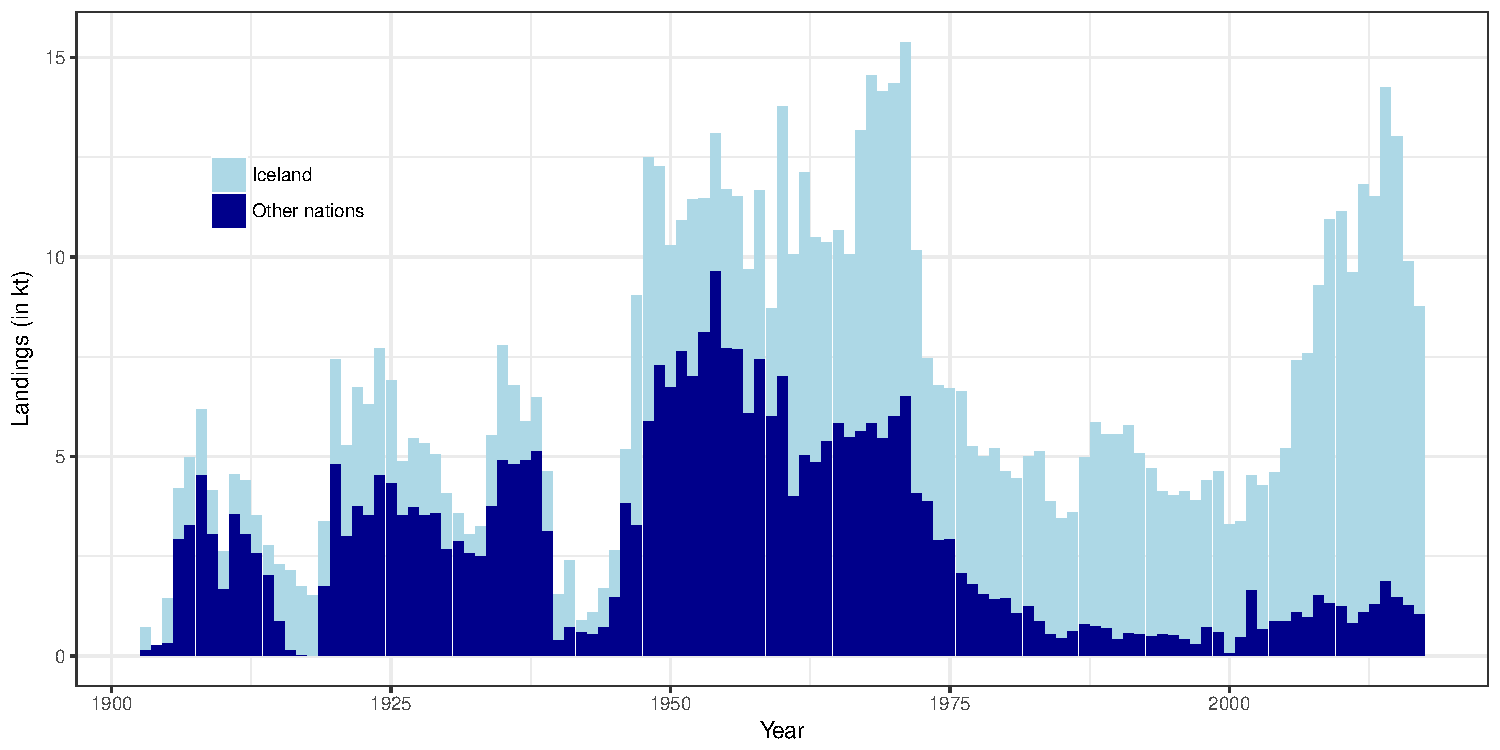
\includegraphics[width=\maxwidth]{figure/landingsplot-1} 

\end{frame}

\begin{frame}
\frametitle{Ling landings by depth}

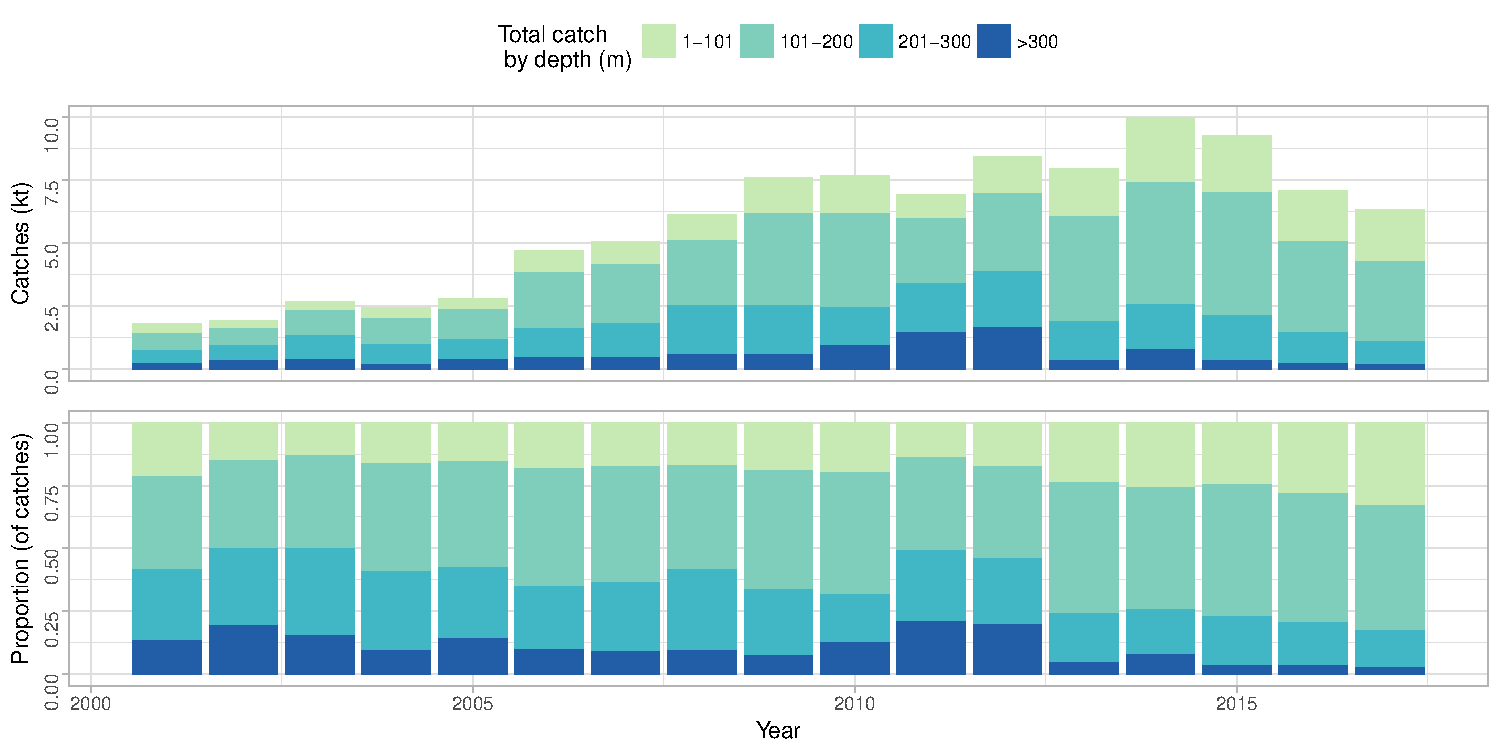
\includegraphics[width=\maxwidth]{figure/depthdistplot-1} 

\end{frame}


\begin{frame}
\frametitle{Ling landings by gear}

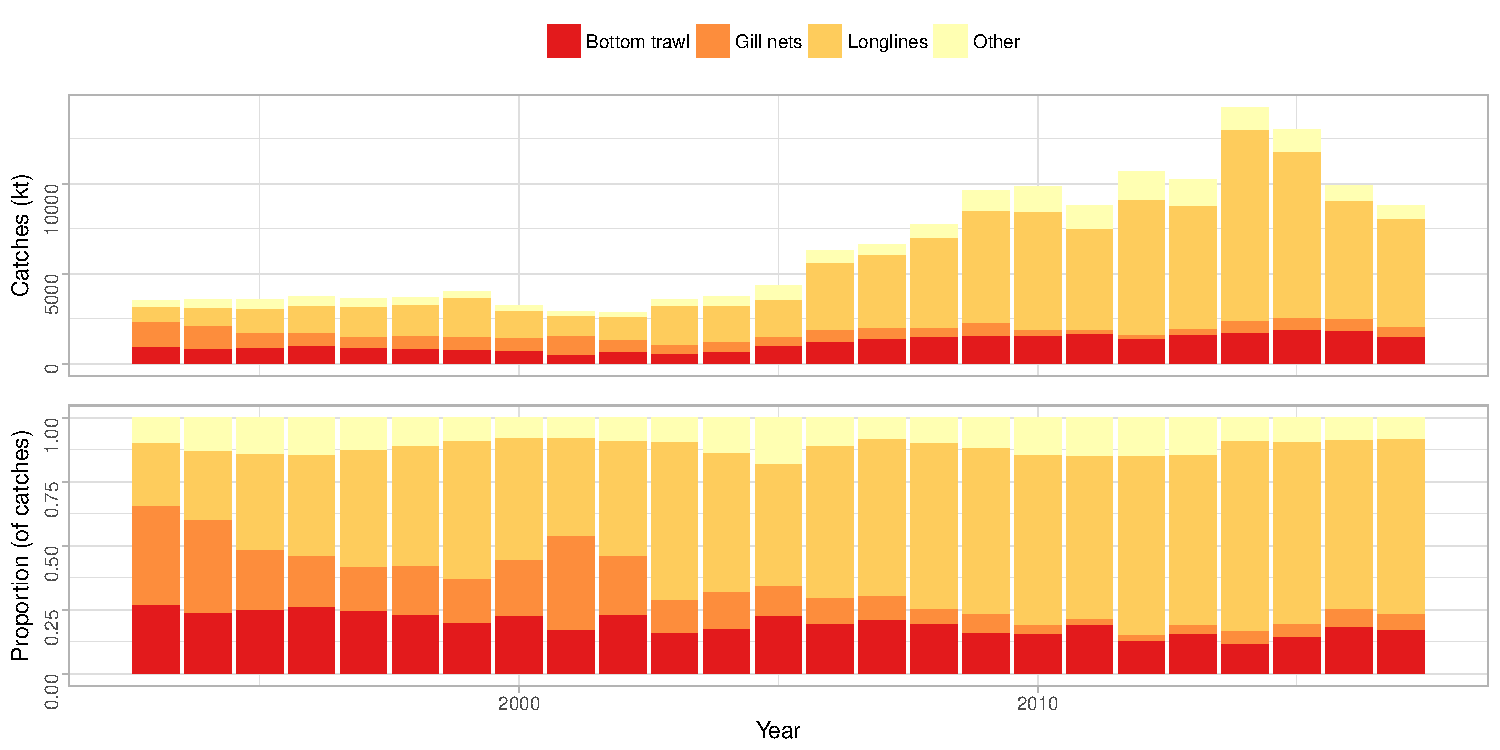
\includegraphics[width=\maxwidth]{figure/catchdistplot-1} 

\end{frame}

\begin{frame}
\frametitle{Ling landings spatial distribution}

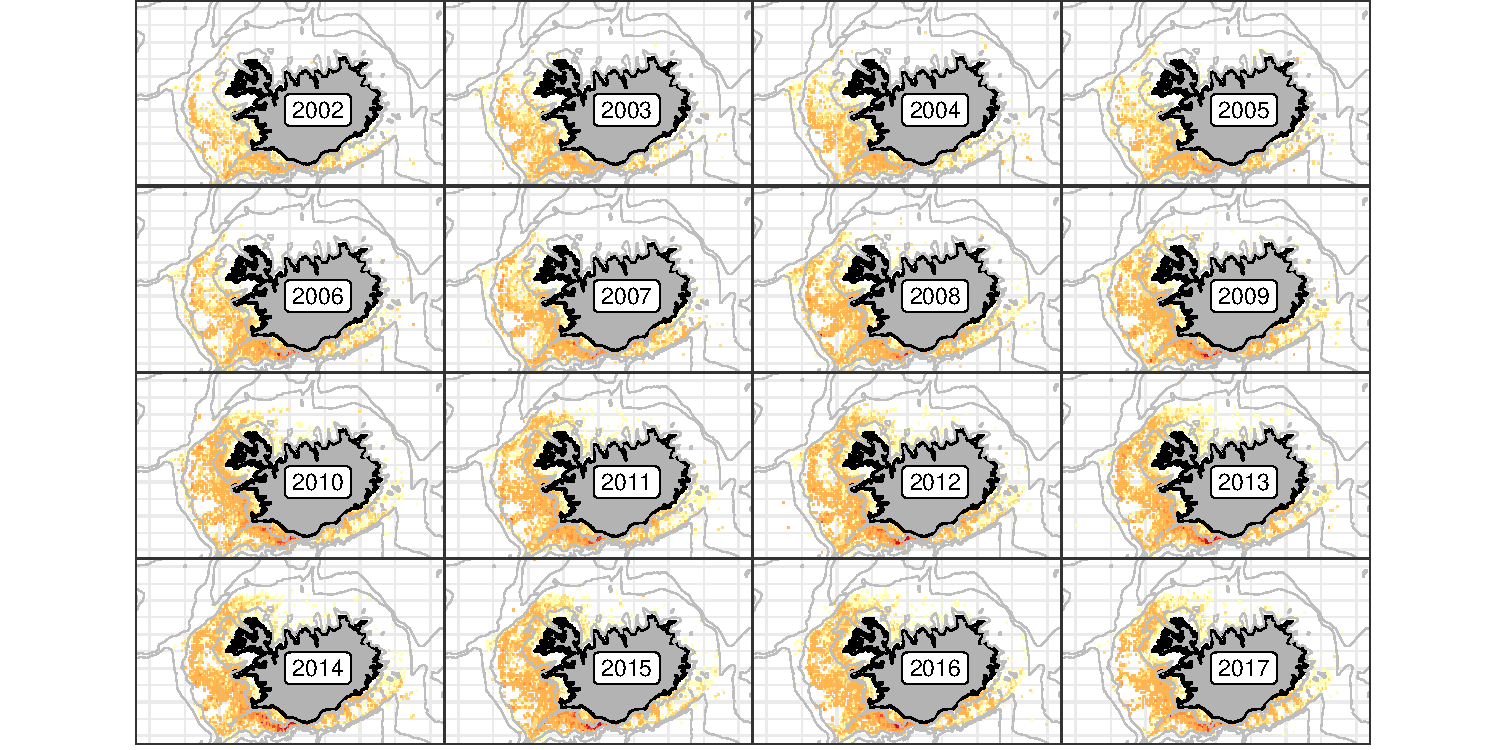
\includegraphics[width=\maxwidth]{figure/catchspatdistplot-1} 

\end{frame}

\begin{frame}
\frametitle{Ling landings by region}

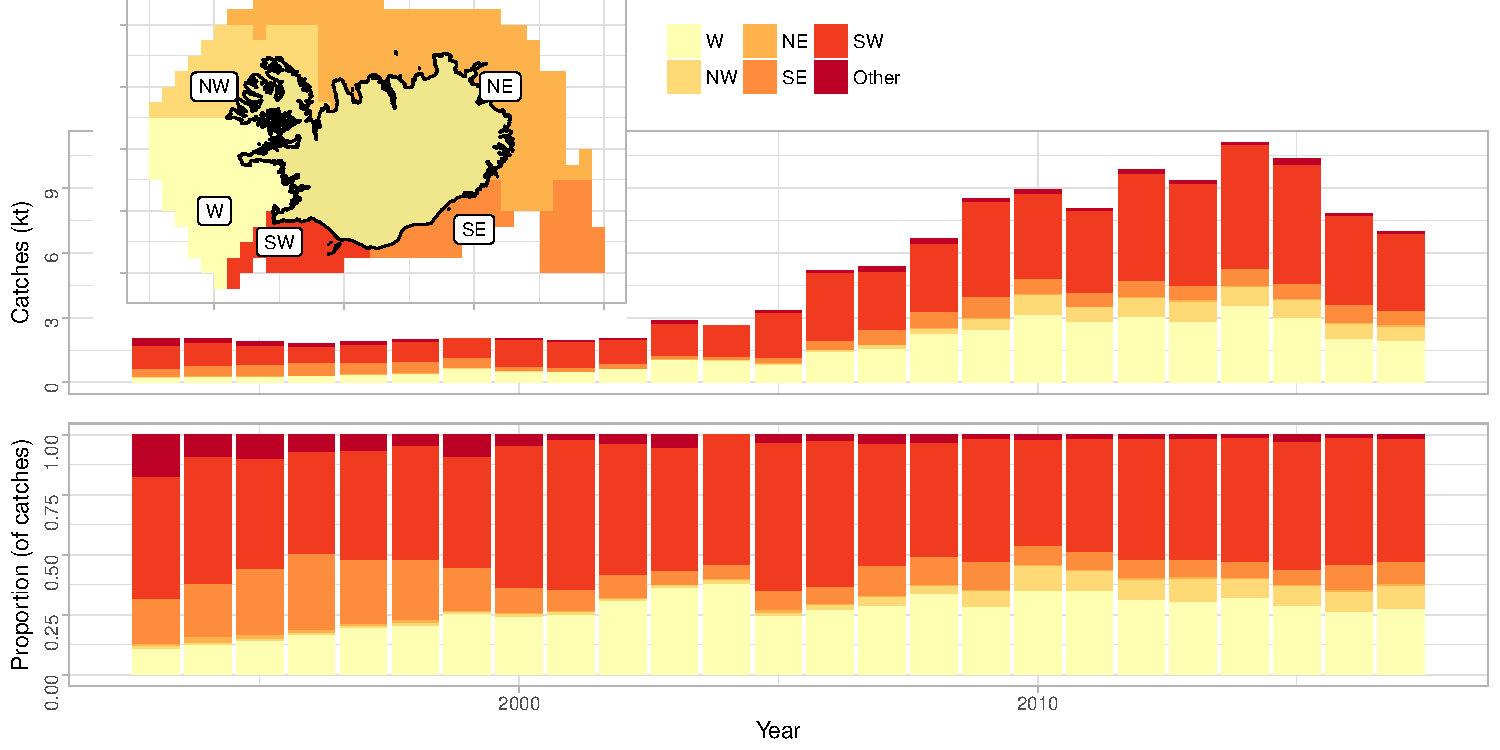
\includegraphics[width=\maxwidth]{figure/catchbyregion-1} 

\end{frame}

\frame{
\frametitle{Accepted management plan}
\begin{knitrout}
\definecolor{shadecolor}{rgb}{0.969, 0.969, 0.969}\color{fgcolor}
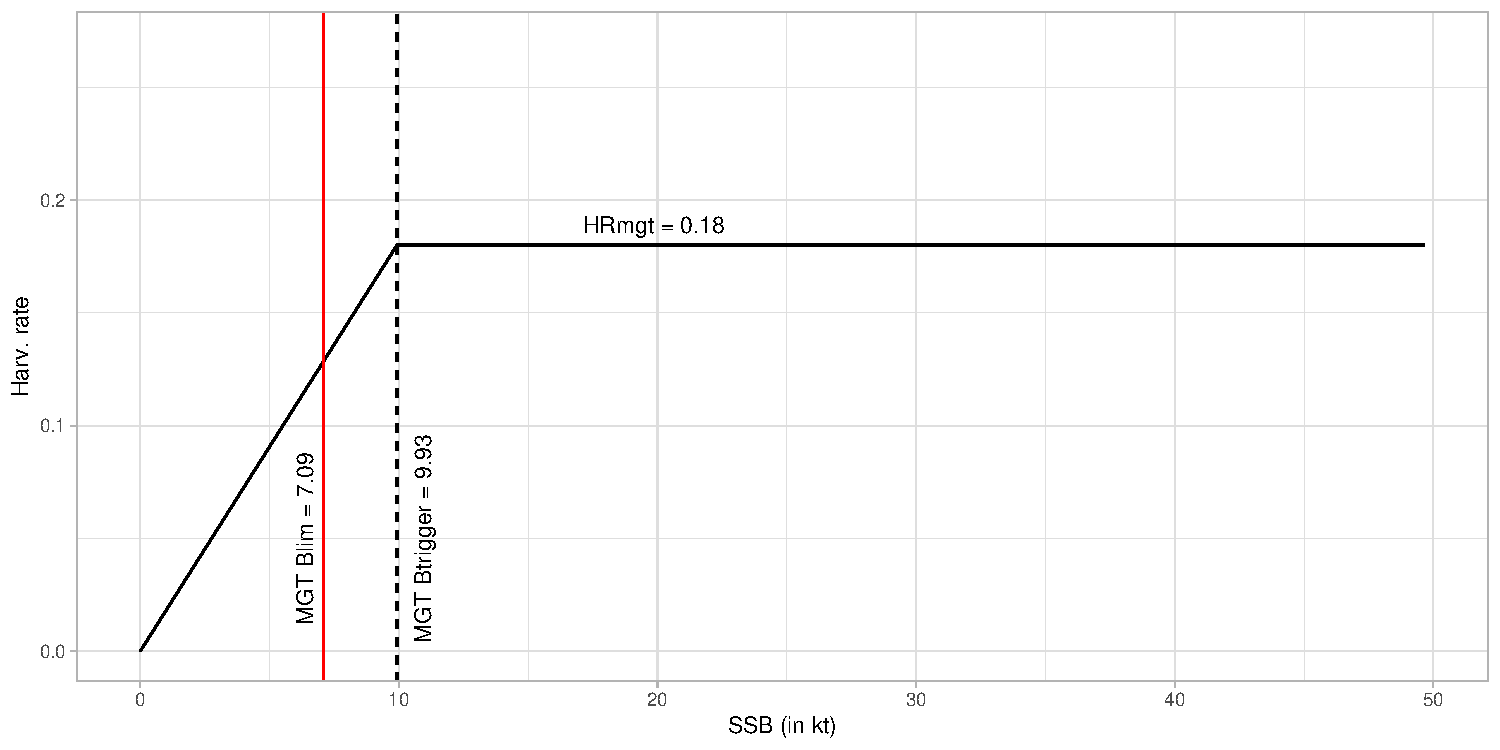
\includegraphics[width=\maxwidth]{figure/mp_plot-1} 

\end{knitrout}

}

%\section{Ices advice}
\begin{frame}
\frametitle{The latest Advice from ICES in May 2017 states:}

{\large
\textit{ICES advised that when the management plan is applied, catches in the
   2017/2018 fishing year should be no more than 8 598 tonnes. All catches are assumed
   to be landed.}
\par}
\end{frame}

%THIS ONE DOES NOT COMPILE WELL
% %\section{Management}
% \begin{frame}[fragile]
% \frametitle{Management in Iceland (Va)}
% {\centering
% \tiny
% \begin{tabular}{lccccc}
% \toprule
% \mcol{1}{l}{Fishing}&\mcol{1}{l}{MRI}&\mcol{1}{l}{National}&\mcol{1}{l}{Landings}\\ 
% \mcol{1}{l}{year} &\mcol{1}{l}{advice}&\mcol{1}{l}{TAC}&       \\
% \midrule
% 1999/00    &          &            &   3961\\
% 2000/01    &          &            &   3451\\
% 2001/02    &      3000&        3000&   2968\\
% 2002/03    &      3000&        3000&   3715\\
% 2003/04    &      3000&        3000&   4608\\
% 2004/05    &      4000&        4000&   5238\\
% 2005/06    &      4500&        5000&   6961\\
% 2006/07    &      5000&        5000&   7617\\
% 2007/08    &      6000&        7000&   8560\\
% 2008/09    &      6000&        7000&   10489\\ 
% 2009/10    &      6000&        7000&   10713\\
% 2010/11    &      7500&        7500&   10095 \\
% 2011/12    &      8800&        9000&   11133\\
% 2012/13    &     12000&       11500&   12445\\
% 2013/14    &     14000&       13500&   13470\\
% 2014/15    &     14300&       13800&   13166\\
% 2015/16    &     16200&       15000&    9769\\
% 2016/17    &      9343&        8143\\
% \bottomrule
% \end{tabular}
% \par}
%\end{frame}

 \begin{frame}
 \frametitle{Management of ling in Iceland (Va)}
 {\centering

\begin{tabular}{l|l|l|l}
\hline
Fishing Year & MFRI Advice & National TAC & Landings\\
\hline
1999/00 &  &  & 3961\\
\hline
2000/01 &  &  & 3451\\
\hline
2001/02 & 3000 & 3000 & 2968\\
\hline
2002/03 & 3000 & 3000 & 3715\\
\hline
2003/04 & 3000 & 3000 & 4608\\
\hline
2004/05 & 4000 & 4000 & 5238\\
\hline
2005/06 & 4500 & 5000 & 6961\\
\hline
2006/07 & 5000 & 5000 & 7617\\
\hline
2007/08 & 6000 & 7000 & 8560\\
\hline
2008/09 & 6000 & 7000 & 10489\\
\hline
2009/10 & 6000 & 7000 & 10713\\
\hline
2010/11 & 7500 & 7500 & 10095\\
\hline
2011/12 & 8800 & 9000 & 11133\\
\hline
2012/13 & 12000 & 11500 & 12445\\
\hline
2013/14 & 14000 & 13500 & 13470\\
\hline
2014/15 & 14300 & 13800 & 13166\\
\hline
2015/16 & 16200 & 15000 & 9769\\
\hline
2016/17 & 9343 & 8143 & 8336\\
\hline
2017/18 & 8598 & 8598 & \\
\hline
\end{tabular}


\par}
\end{frame}

\begin{frame}
\frametitle{Transfers in the Icelandic ITQ-system}
% {\centering
% 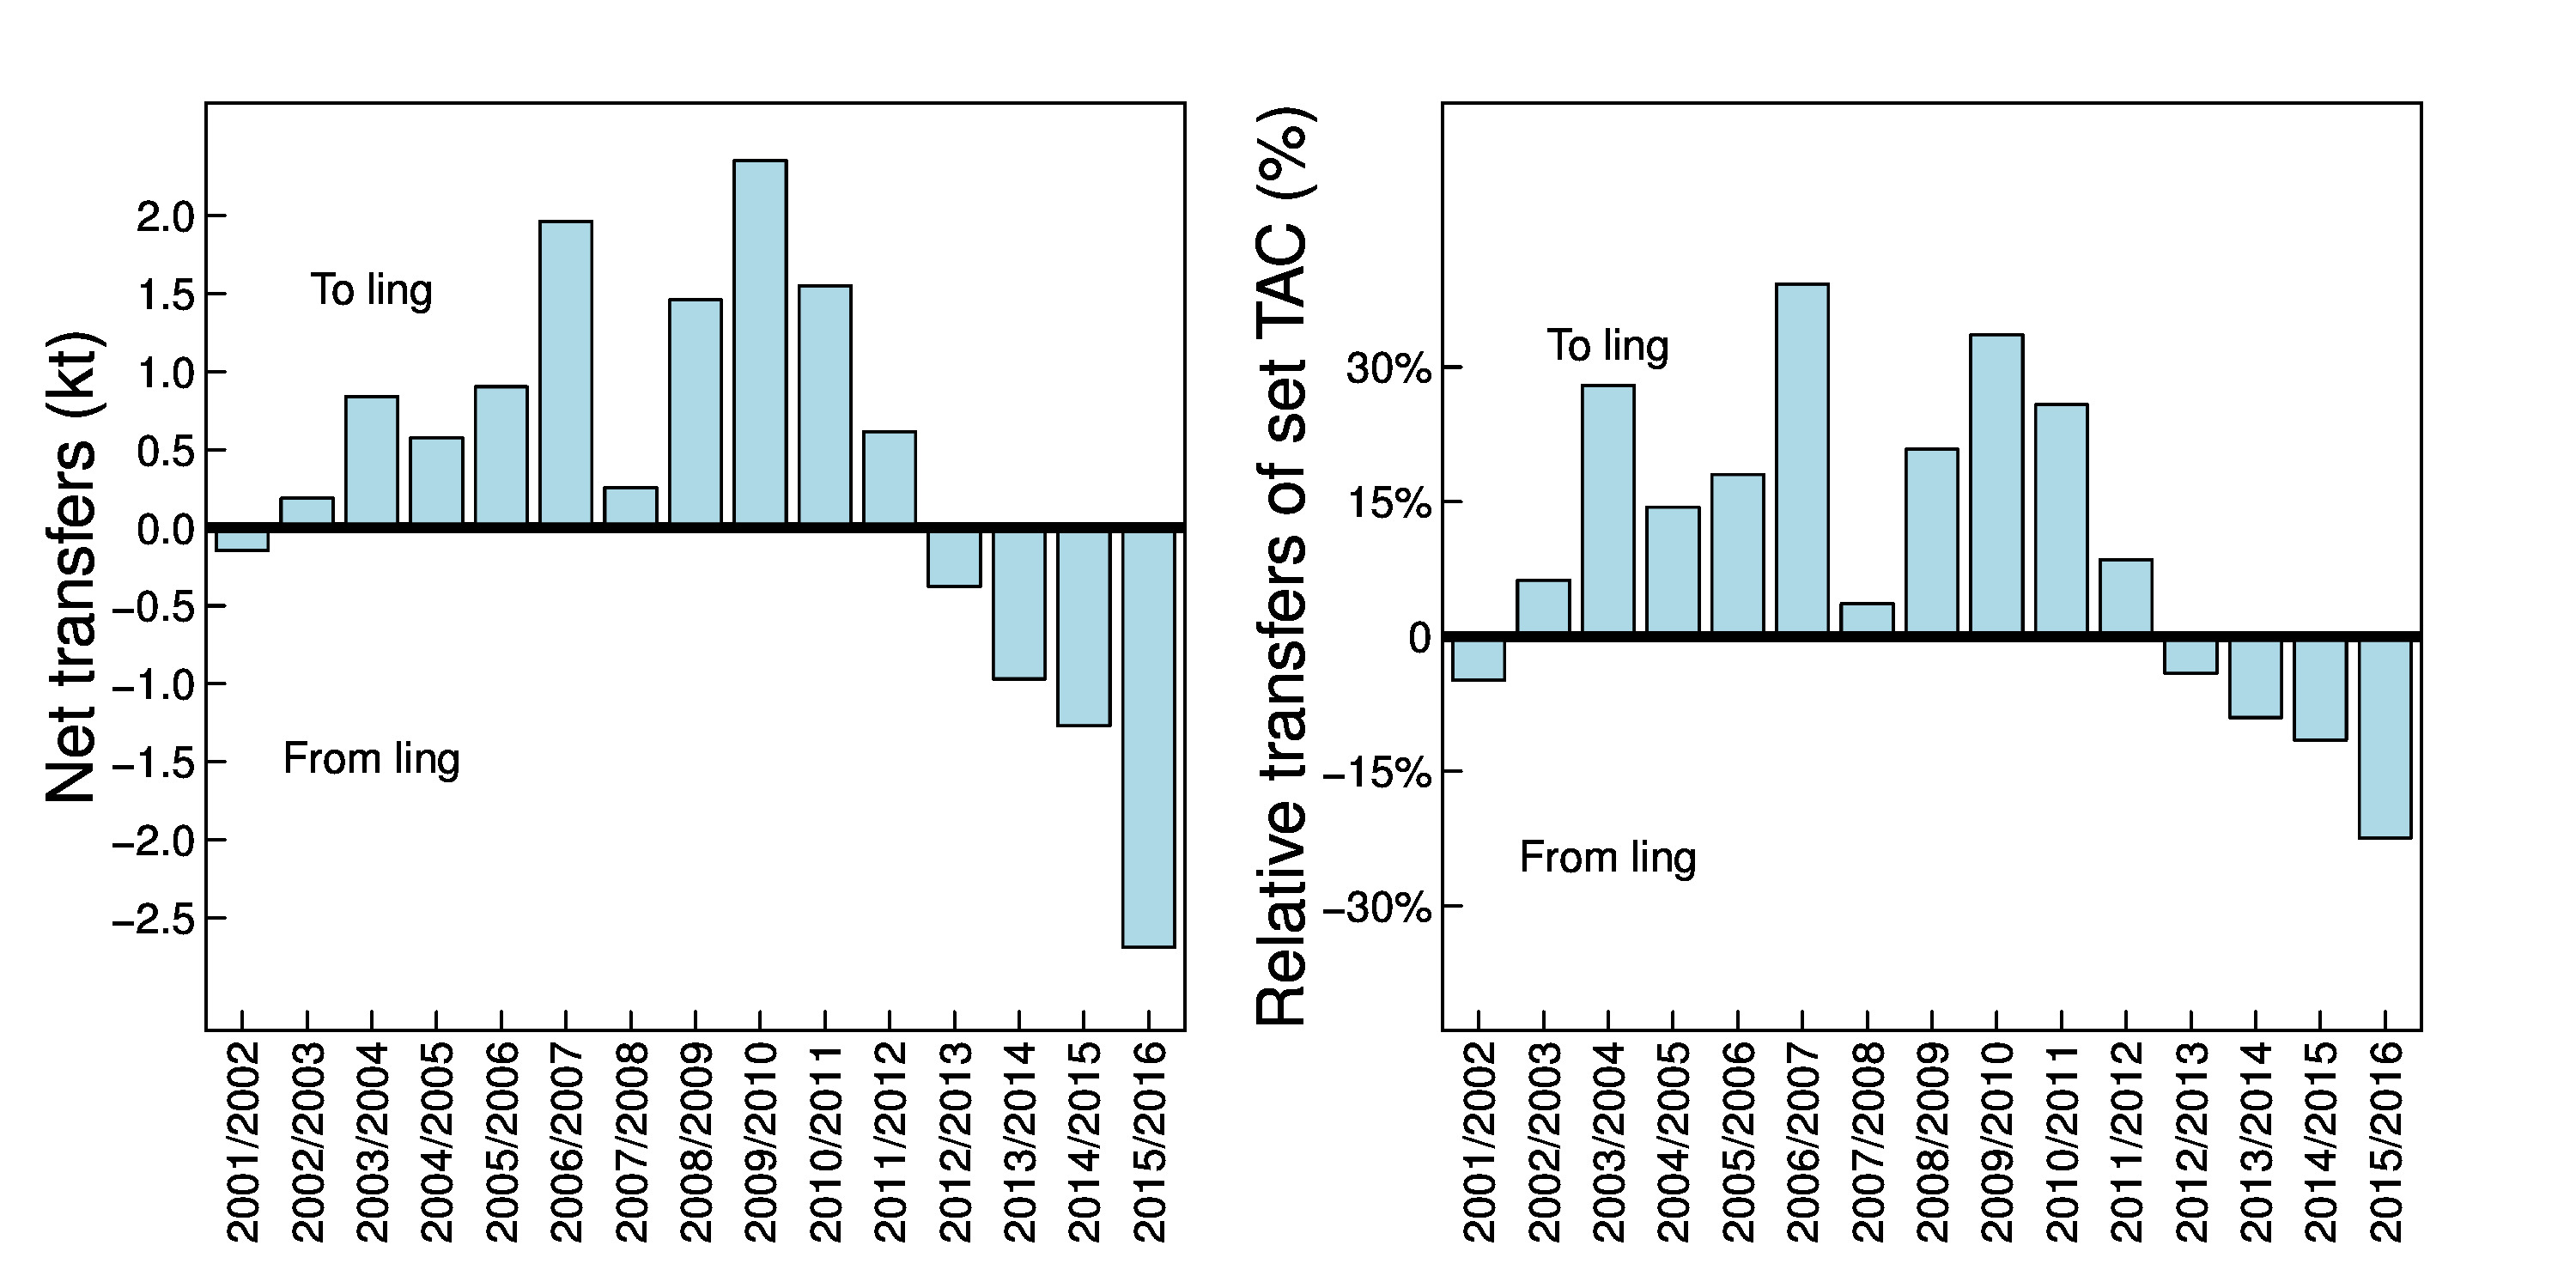
\includegraphics[width=0.8\linewidth, angle=0]{LingQuotaTransfer.jpg}
% \par}


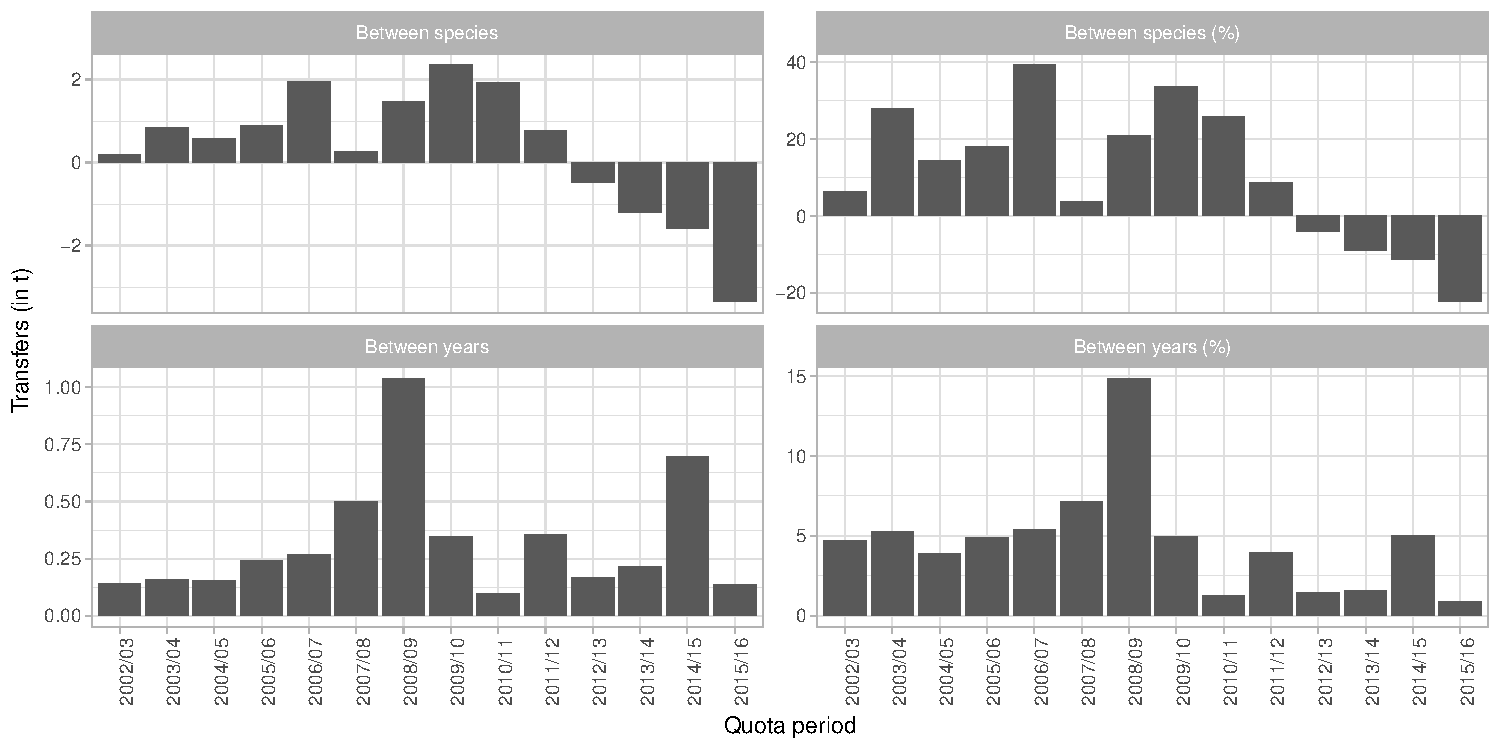
\includegraphics[width=\maxwidth]{figure/transfplot-1} 


\end{frame}


\begin{frame}
\frametitle{Trends in biomass and juvenile abundance}

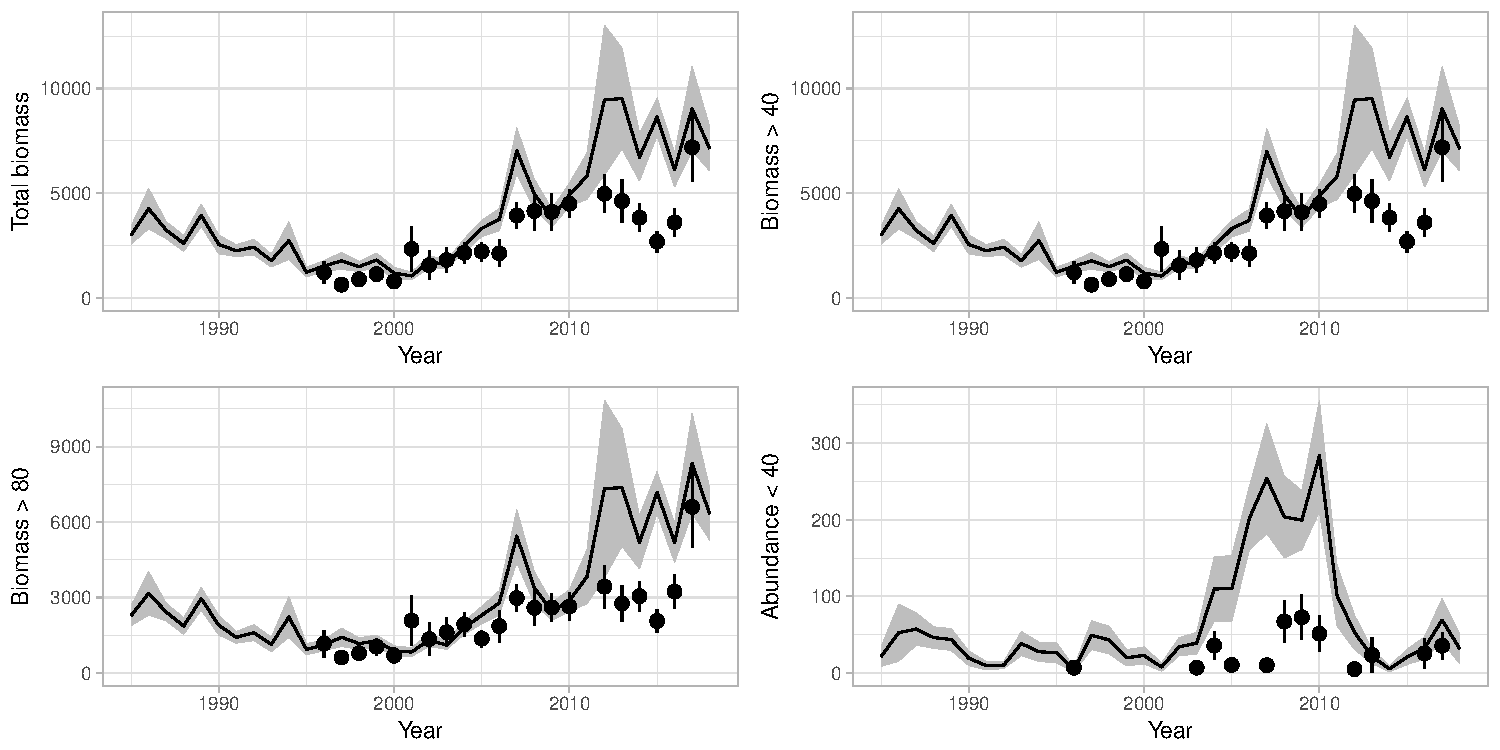
\includegraphics[width=\maxwidth]{figure/biomIndplot-1} 

\end{frame}



\frame{
\frametitle{Observational data for Gadget length- and age-based model}
\bi Survey indices from the Icelandic groundfish survey from 1985, split into 7 slices in ~10 cm intervals.
  \bi lengths 20--160 cm in 4 cm bins
  \item ages 3--15
\ei
\item Survey samples from 1985 (as available):
  \bi proportion at length
  \item proportion at length and age
  \item proportion mature at length
  \ei
\item Commercial samples from 1982 (as available - longlines, gillnets, bottom trawl fleets)
\bi proportion at length by gear
\item proportion at length and age by gear
\ei
\item Commercial catches by gear since 1982
\ei
}


\frame{
\frametitle{Fit to data -- Indices}


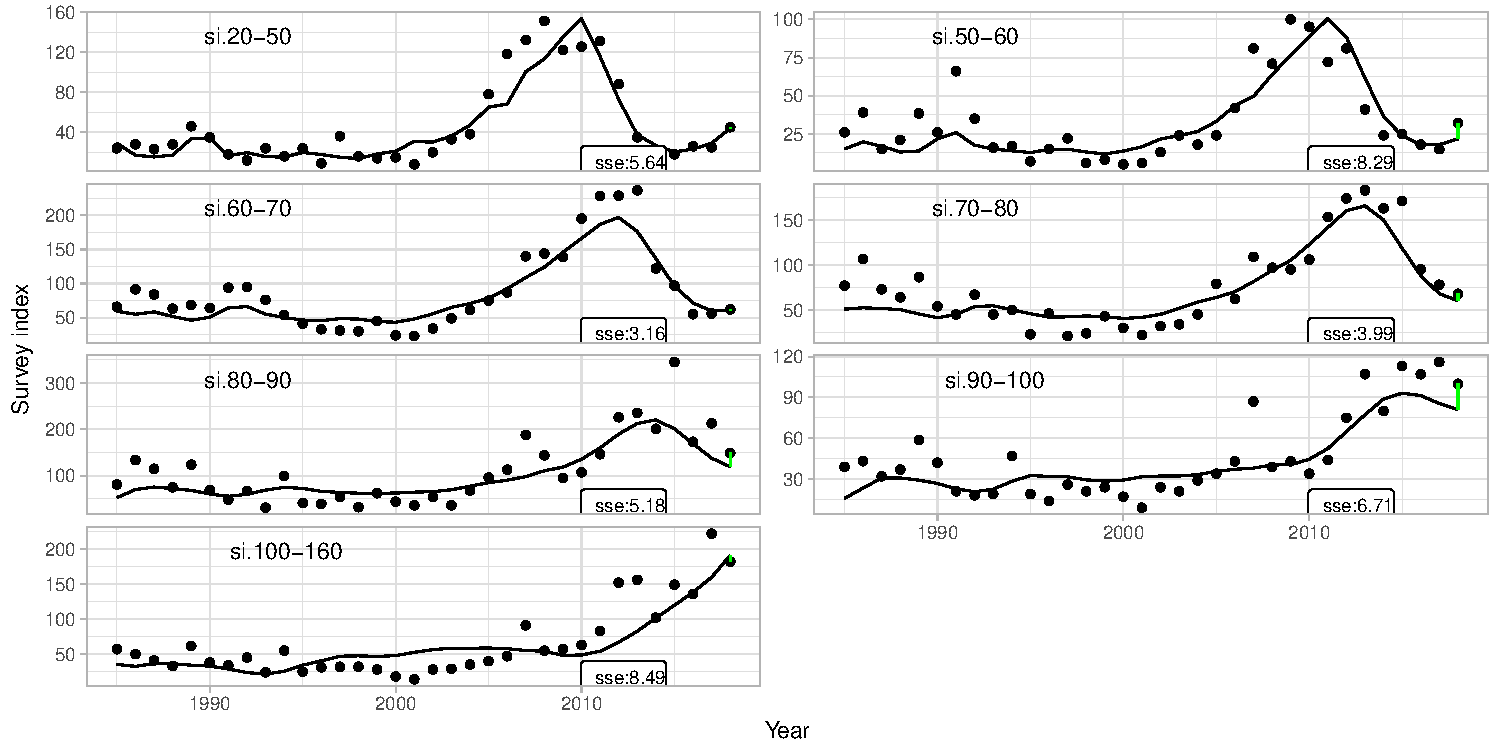
\includegraphics[width=\maxwidth]{figure/unnamed-chunk-6-1} 


}


\frame{
\frametitle{Fit to length distributions}
\begin{knitrout}
\definecolor{shadecolor}{rgb}{0.969, 0.969, 0.969}\color{fgcolor}
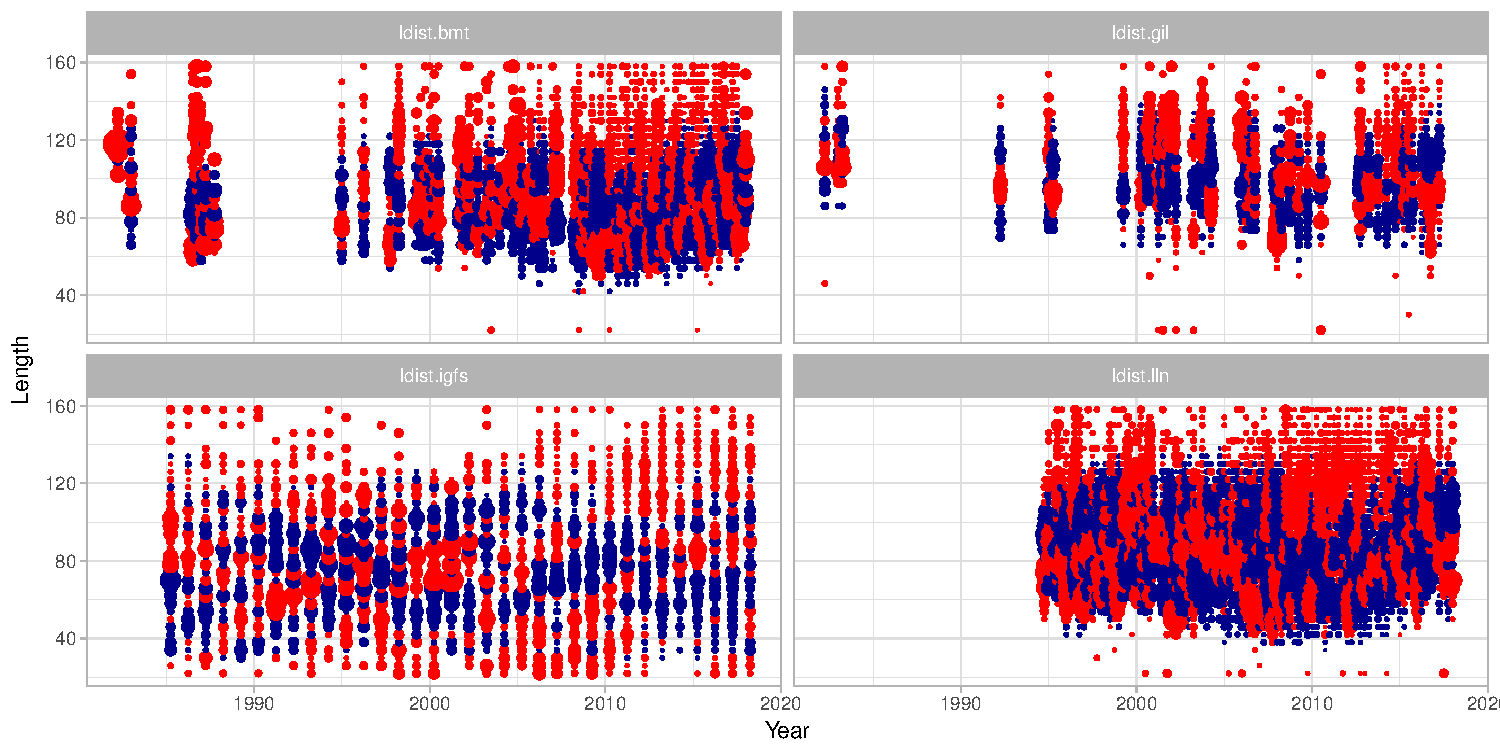
\includegraphics[width=\maxwidth]{figure/bubbleplot-1} 

\end{knitrout}

}

\frame{
\frametitle{Fit to data -- survey length distributions}
\begin{knitrout}
\definecolor{shadecolor}{rgb}{0.969, 0.969, 0.969}\color{fgcolor}
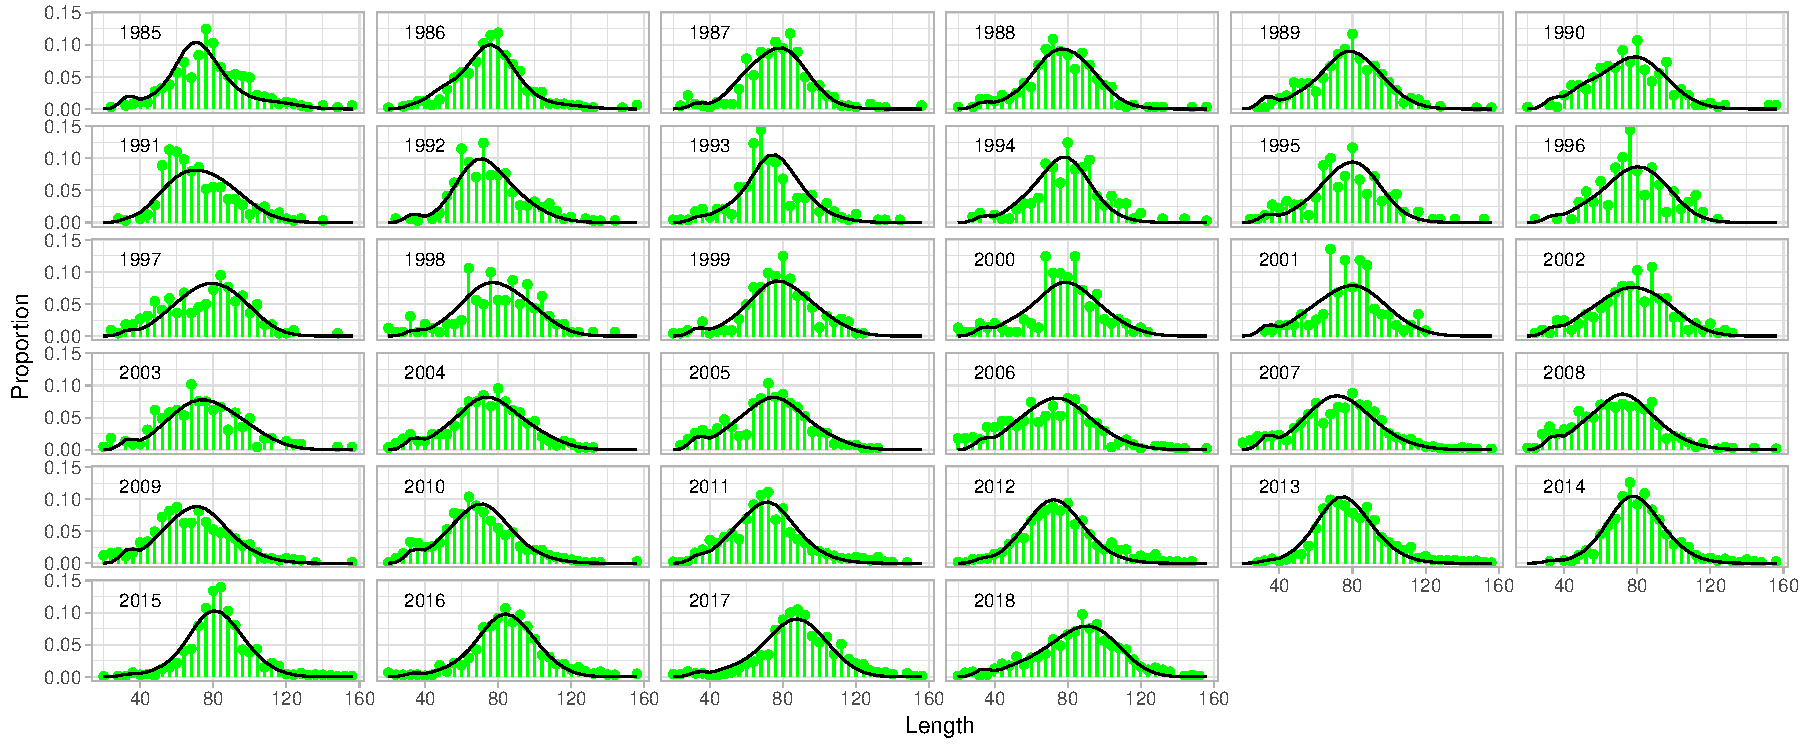
\includegraphics[width=\maxwidth]{figure/unnamed-chunk-7-1} 

\end{knitrout}
}

\frame{
\frametitle{Fit to data -- longline length distributions}
\begin{knitrout}
\definecolor{shadecolor}{rgb}{0.969, 0.969, 0.969}\color{fgcolor}
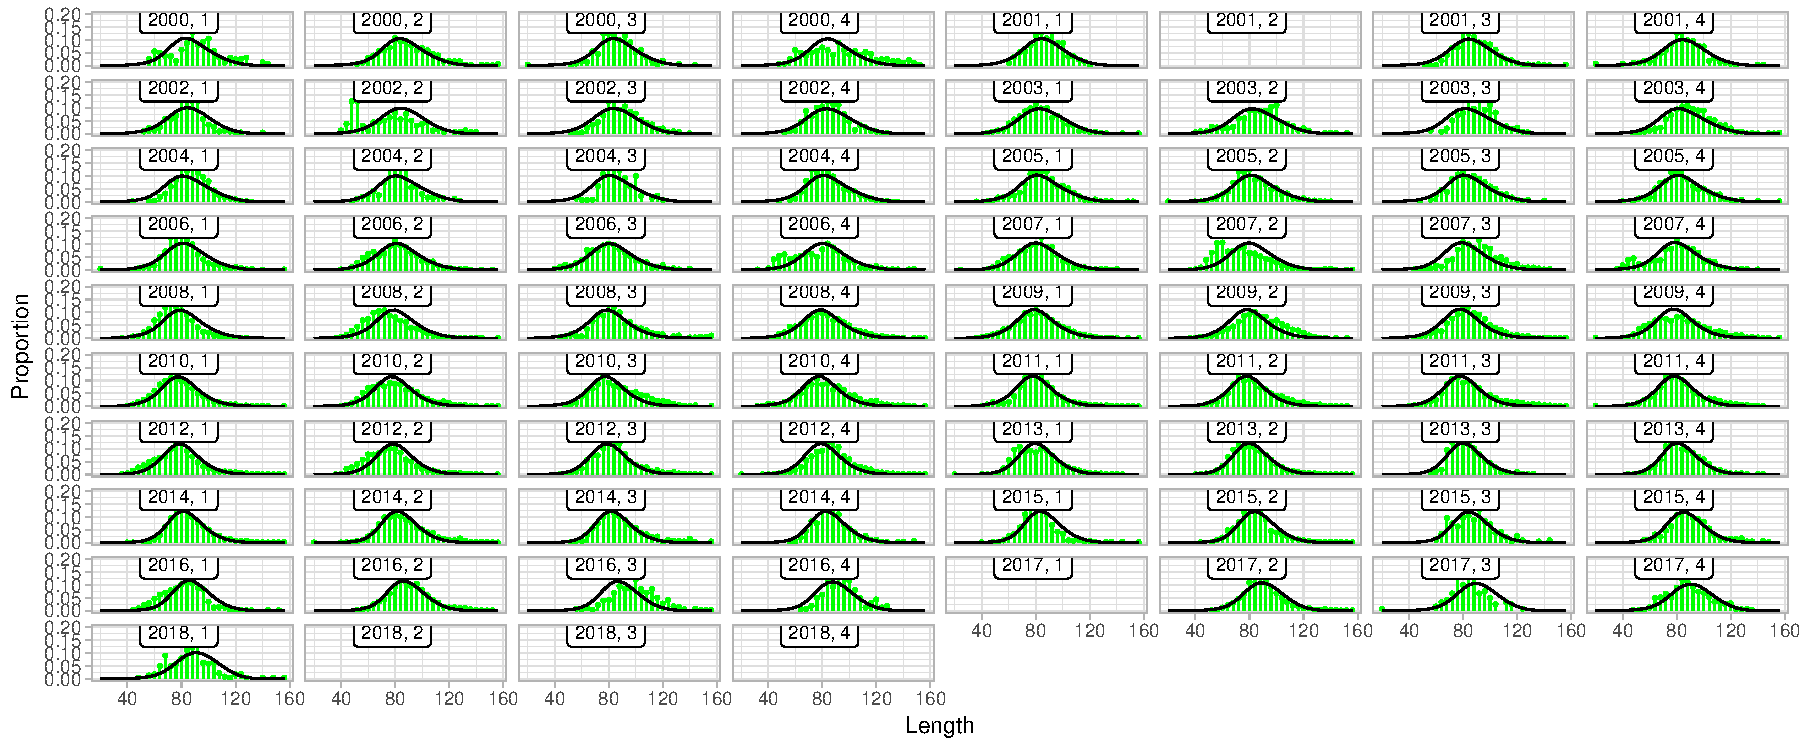
\includegraphics[width=\maxwidth]{figure/unnamed-chunk-8-1} 

\end{knitrout}

}


\frame{
\frametitle{Fit to age distributions}
\begin{knitrout}
\definecolor{shadecolor}{rgb}{0.969, 0.969, 0.969}\color{fgcolor}
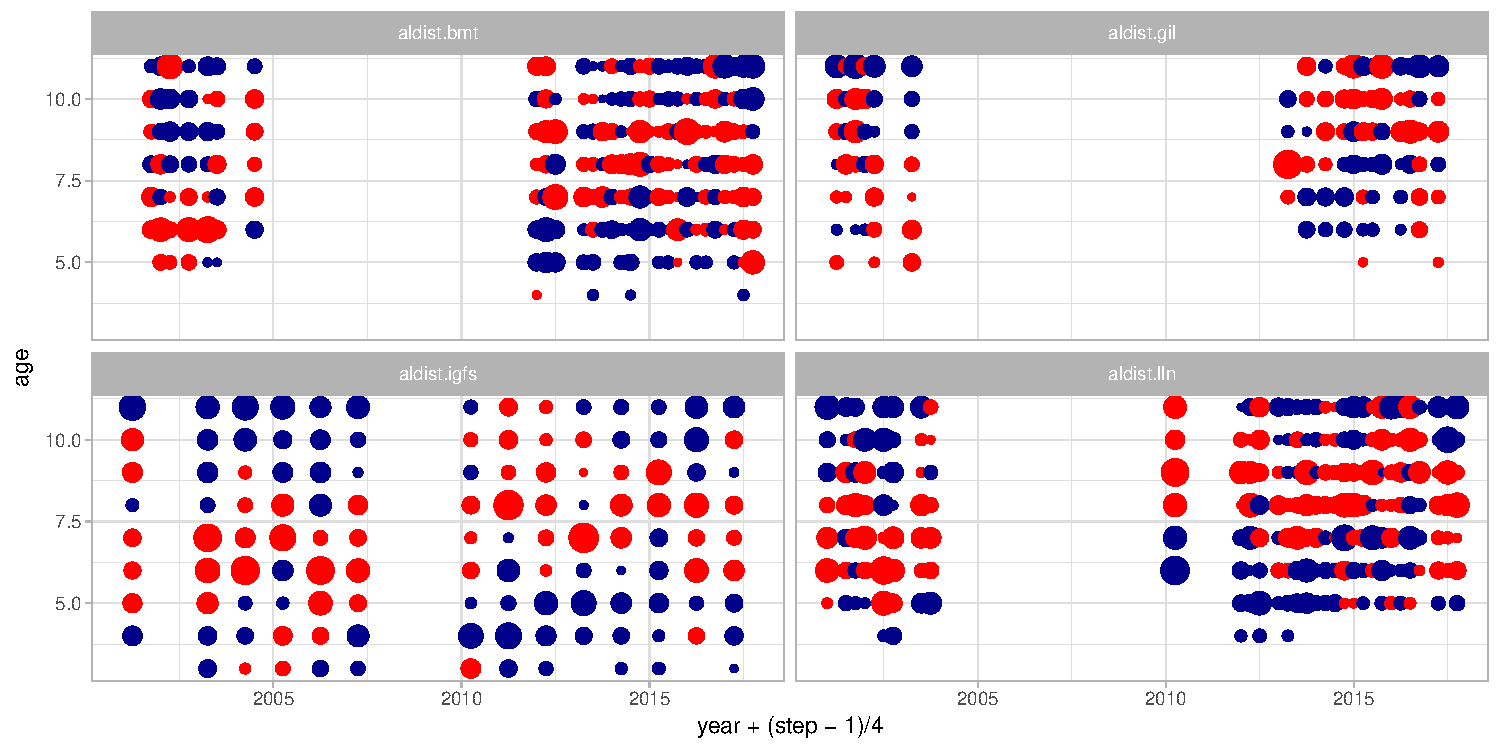
\includegraphics[width=\maxwidth]{figure/agebubbleplot-1} 

\end{knitrout}

}


\frame{
\frametitle{Fit to data -- survey age distributions}
\begin{knitrout}
\definecolor{shadecolor}{rgb}{0.969, 0.969, 0.969}\color{fgcolor}
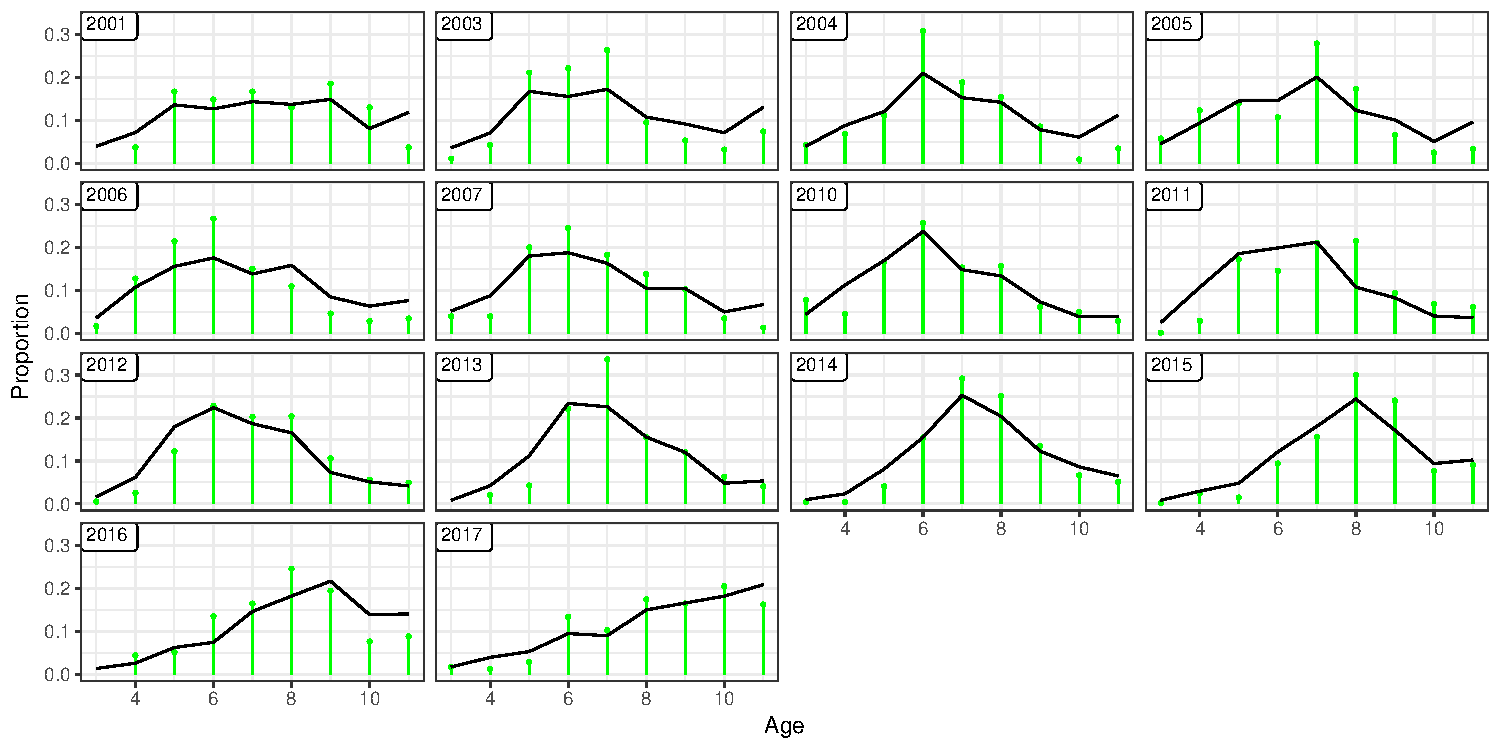
\includegraphics[width=\maxwidth]{figure/unnamed-chunk-9-1} 

\end{knitrout}

}

\frame{
\frametitle{Fit to data -- survey growth data}
\begin{knitrout}
\definecolor{shadecolor}{rgb}{0.969, 0.969, 0.969}\color{fgcolor}
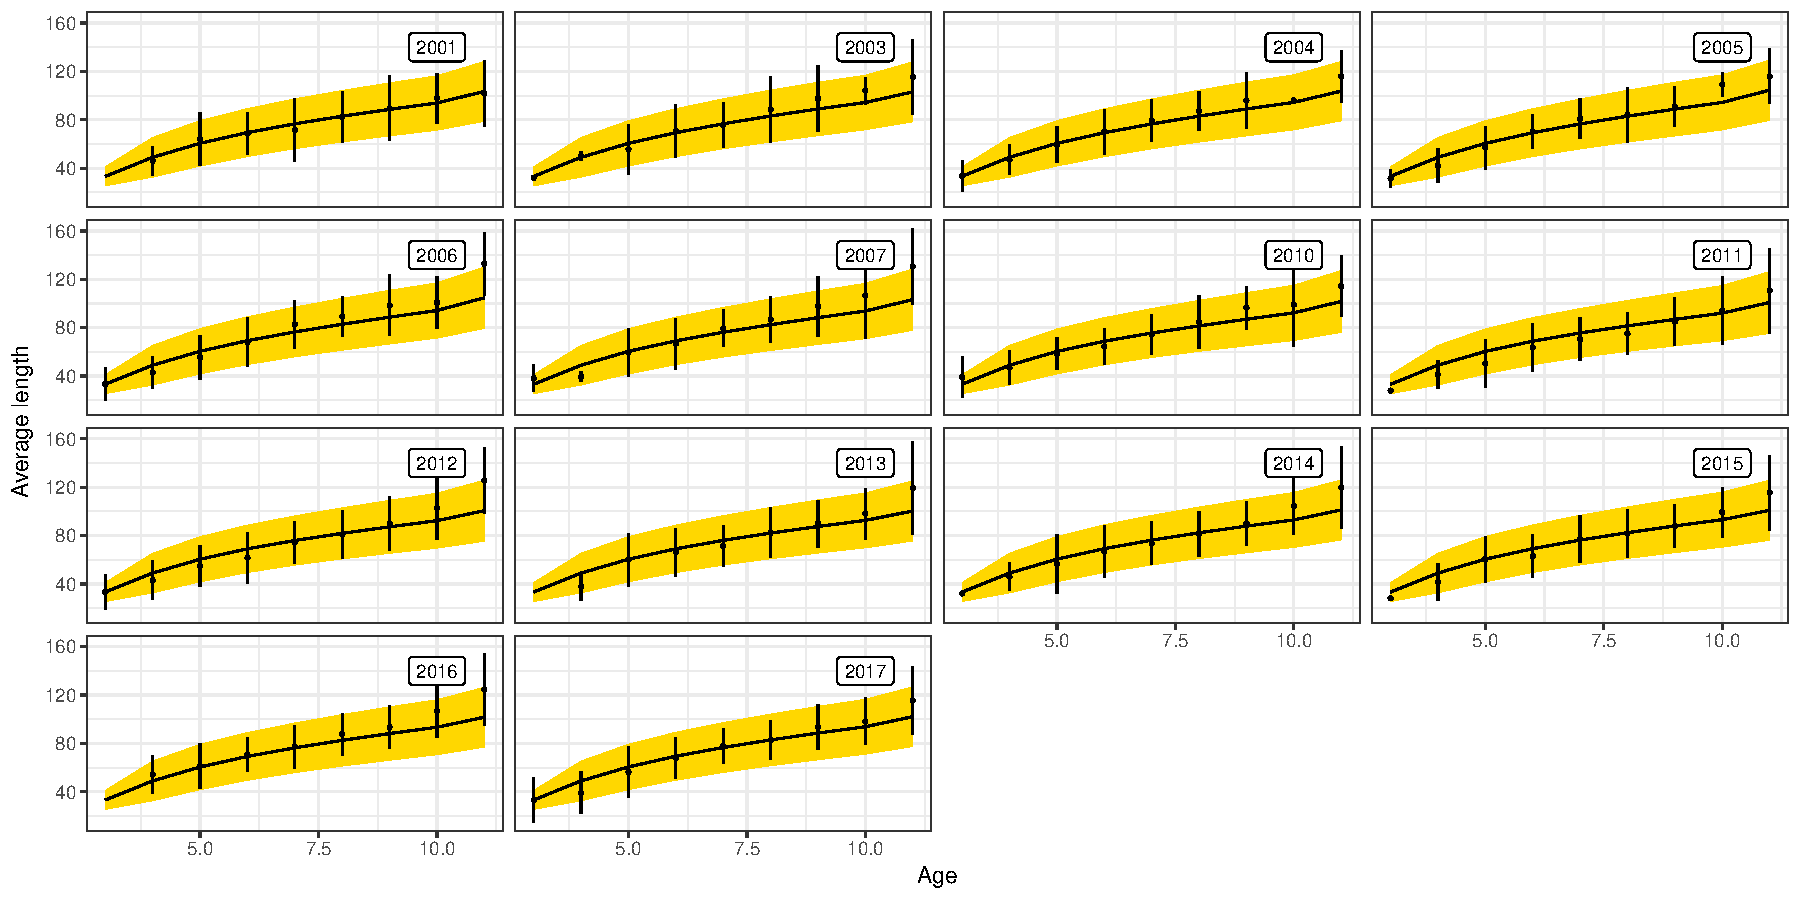
\includegraphics[width=\maxwidth]{figure/unnamed-chunk-10-1} 

\end{knitrout}


}



\frame{
\frametitle{Fit to data -- longline age distributions}
\begin{knitrout}
\definecolor{shadecolor}{rgb}{0.969, 0.969, 0.969}\color{fgcolor}
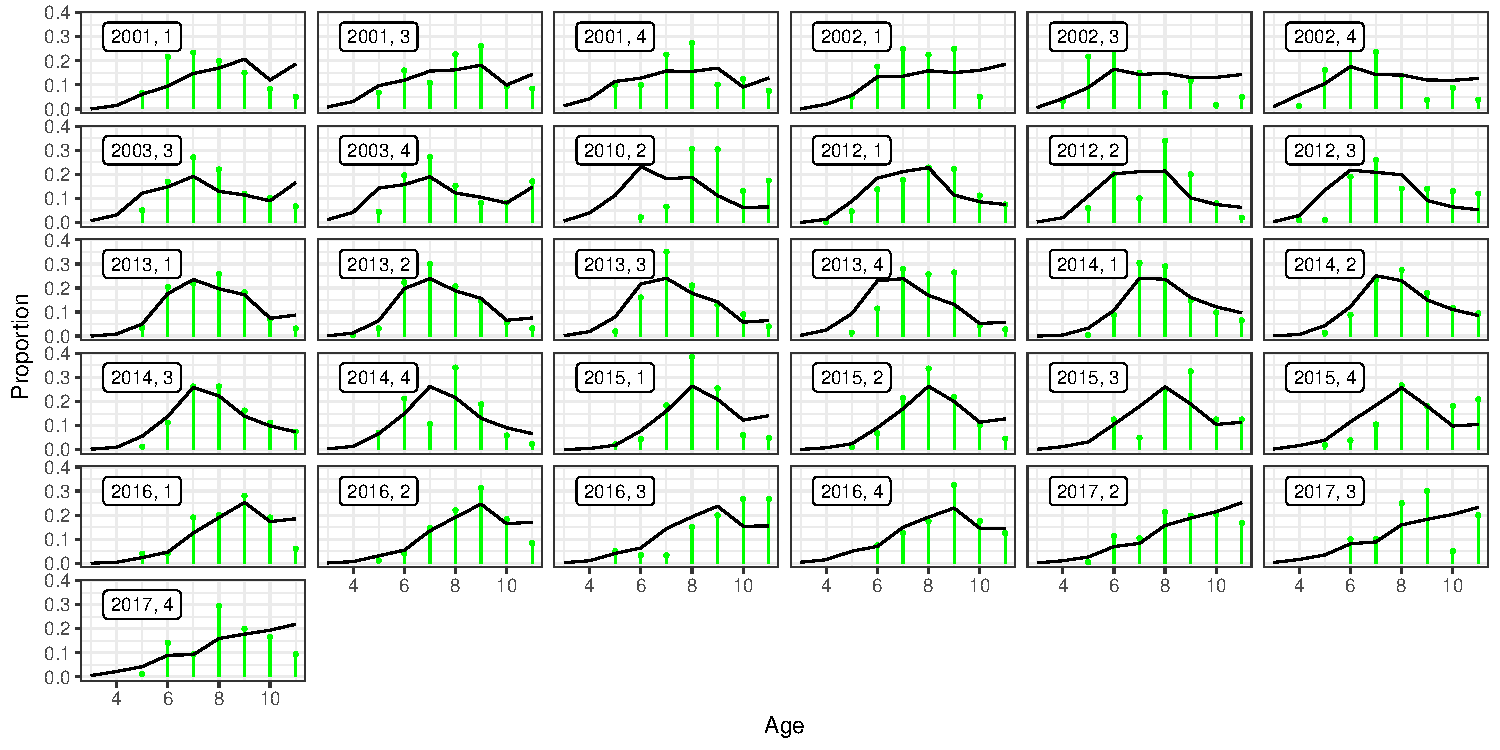
\includegraphics[width=\maxwidth]{figure/unnamed-chunk-11-1} 

\end{knitrout}
}

\frame{
\frametitle{Fit to data -- longline growth data}
\begin{knitrout}
\definecolor{shadecolor}{rgb}{0.969, 0.969, 0.969}\color{fgcolor}
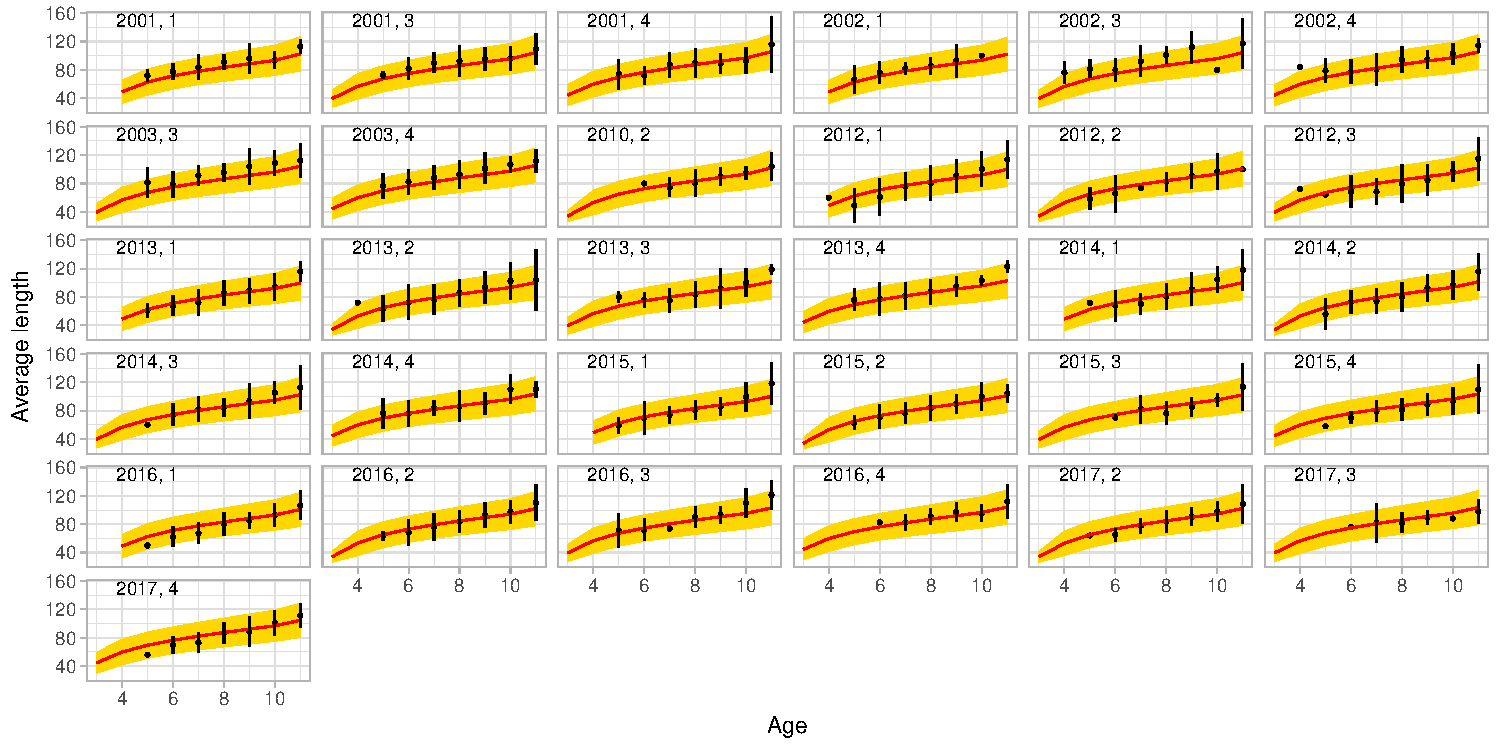
\includegraphics[width=\maxwidth]{figure/unnamed-chunk-12-1} 

\end{knitrout}


}

\frame{
\frametitle{Fit to data -- survey maturity}
\begin{knitrout}
\definecolor{shadecolor}{rgb}{0.969, 0.969, 0.969}\color{fgcolor}
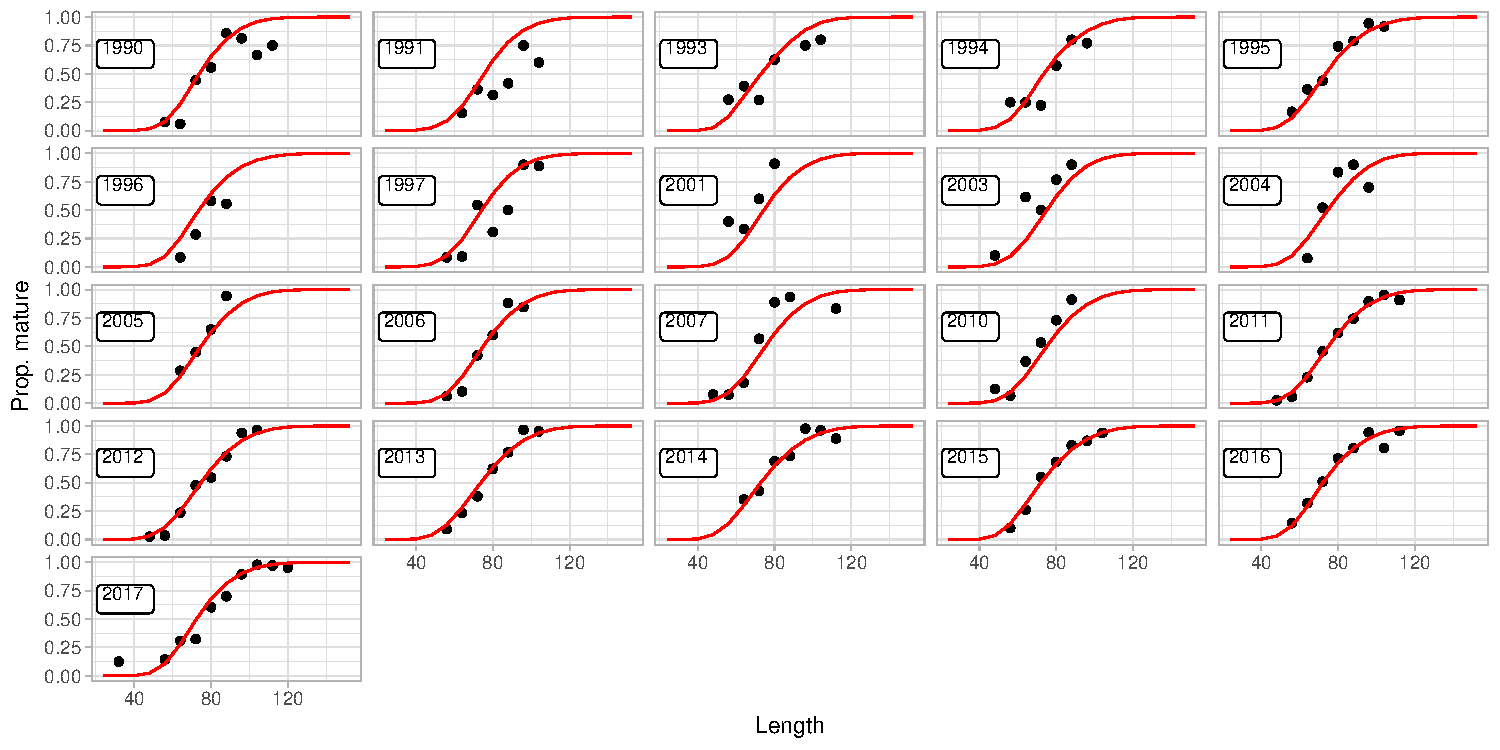
\includegraphics[width=\maxwidth]{figure/unnamed-chunk-13-1} 

\end{knitrout}
}





\begin{table}[!h]
\vspace{1mm}
\caption[]
{Ling in 5a. Summary of reference points for ling in 5a. }\label{tbl:refpoint}
\vspace{2mm}
{\centering
\scriptsize
\begin{tabular}{p{2.5cm} l r p{5cm} }
\toprule
Framework & Reference point & Value & Technical basis \\ \midrule
MSY approach & MSY $B_{trigger}$ &  9.93 kt & $B_{pa}$ \\
            & $H_{msy}$ & 0.24 & The harvest rate that maximises the median long-term catch in stochastic simulations with recruitment drawn from a block bootstrap of historical recruitment scaled according to a hockey stick recruitment function with $B_{loss}$ as defined below.\\
            & $F_{msy}$ & 0.284 & The median fishing mortality when an harvest rate of $H_{msy}$ is applied. \\
%            & $H_{p.05}$ & 0.497 & The harvest rate that has an annual probability of 5\% of SSB < $B_lim$.\\
%            & $F_{p.05}$ & 0.516 &  The median fishing mortality when an harvest rate of $H_{p.05}$ is applied.\\
\hline
Precautionary approach & $B_{lim}$ & 7.09 kt & $B_{pa}/e^{1.645\sigma}$ where $\sigma=0.2$ \\
                      & $B_{pa}$ & 9.93 kt & SSB(1992), corresponding to $B_{loss}$ \\
                      & $H_{lim}$ & 0.56 & $H$ corresponding to 50\% long-term probability of SSB > $B_{lim}$ \\
                      & $F_{lim}$ & 0.70 & F corresponding to $H_{lim}$ \\
                      & $F_{pa}$ &  0.41 & $F_{lim}/e^{1.645\sigma}$ where $\sigma=0.33$\\
                      & $H_{pa}$ & 0.35 & H corresponding to $F_{pa}$ \\
\hline
Management plan & $H_{mp}$ & 0.18 & $H$ such that $P(SSB<B_{pa}|\textup{for any given year})<0.05$. \\
\bottomrule
\end{tabular}
\par}
\end{table}

\frame{
\frametitle{Assessment results}

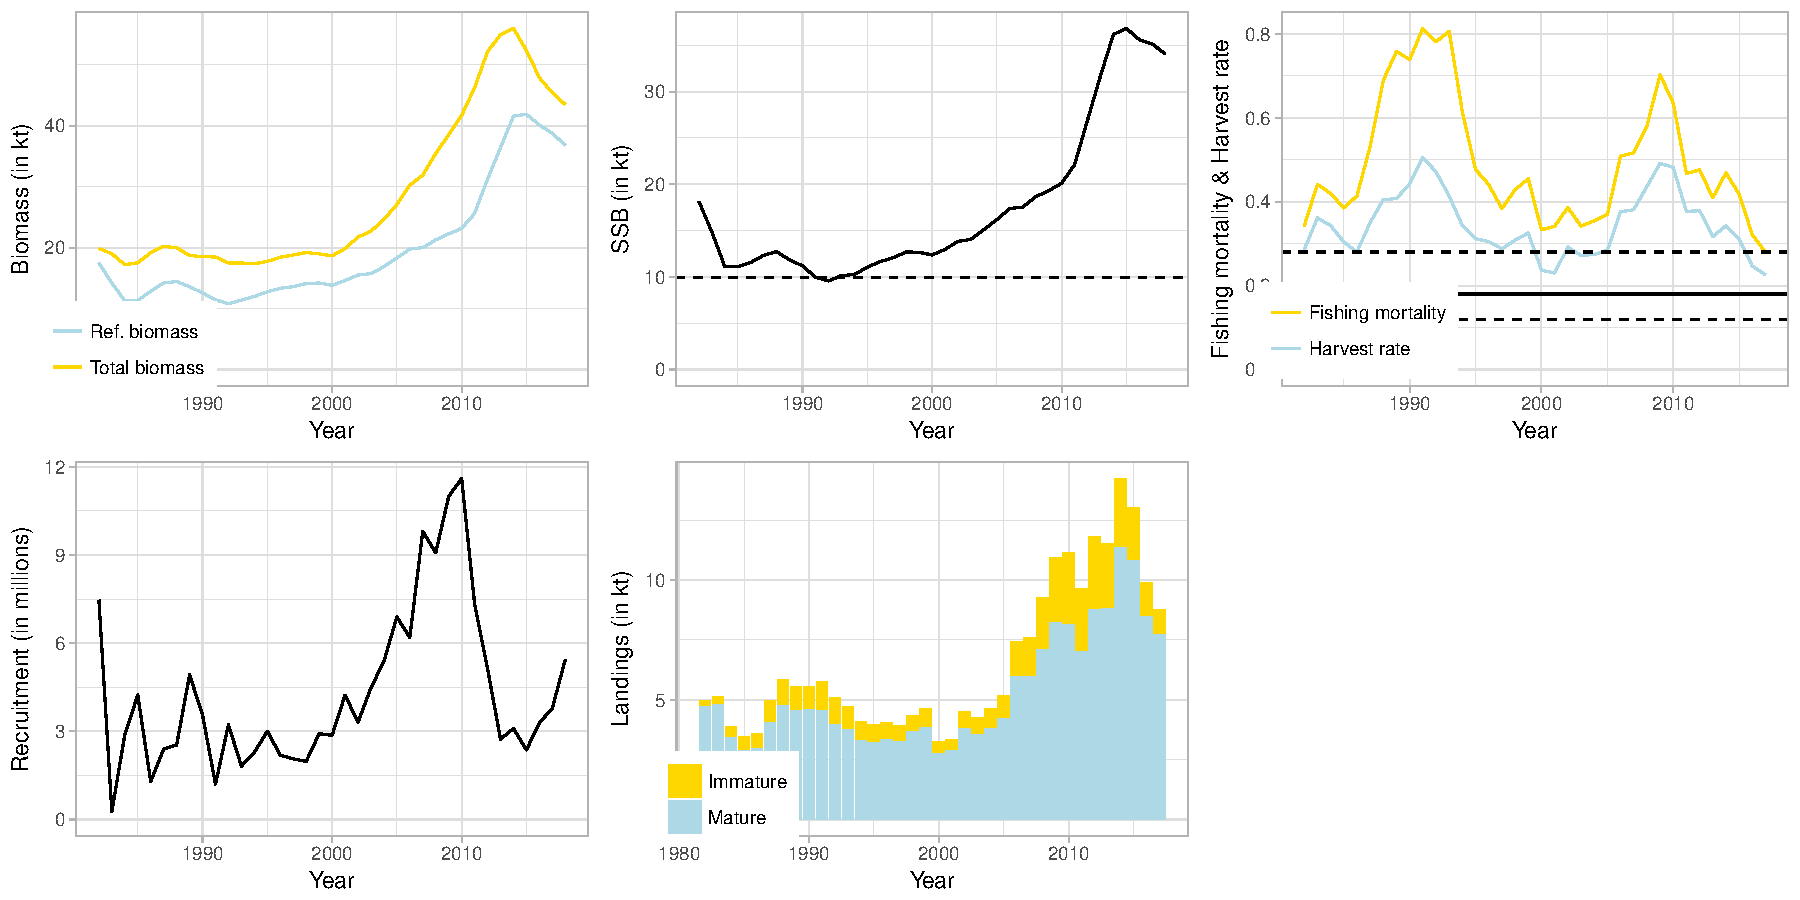
\includegraphics[width=\maxwidth]{figure/unnamed-chunk-14-1} 


}




\frame{
\frametitle{Comparison with previous assessment}
\begin{knitrout}
\definecolor{shadecolor}{rgb}{0.969, 0.969, 0.969}\color{fgcolor}
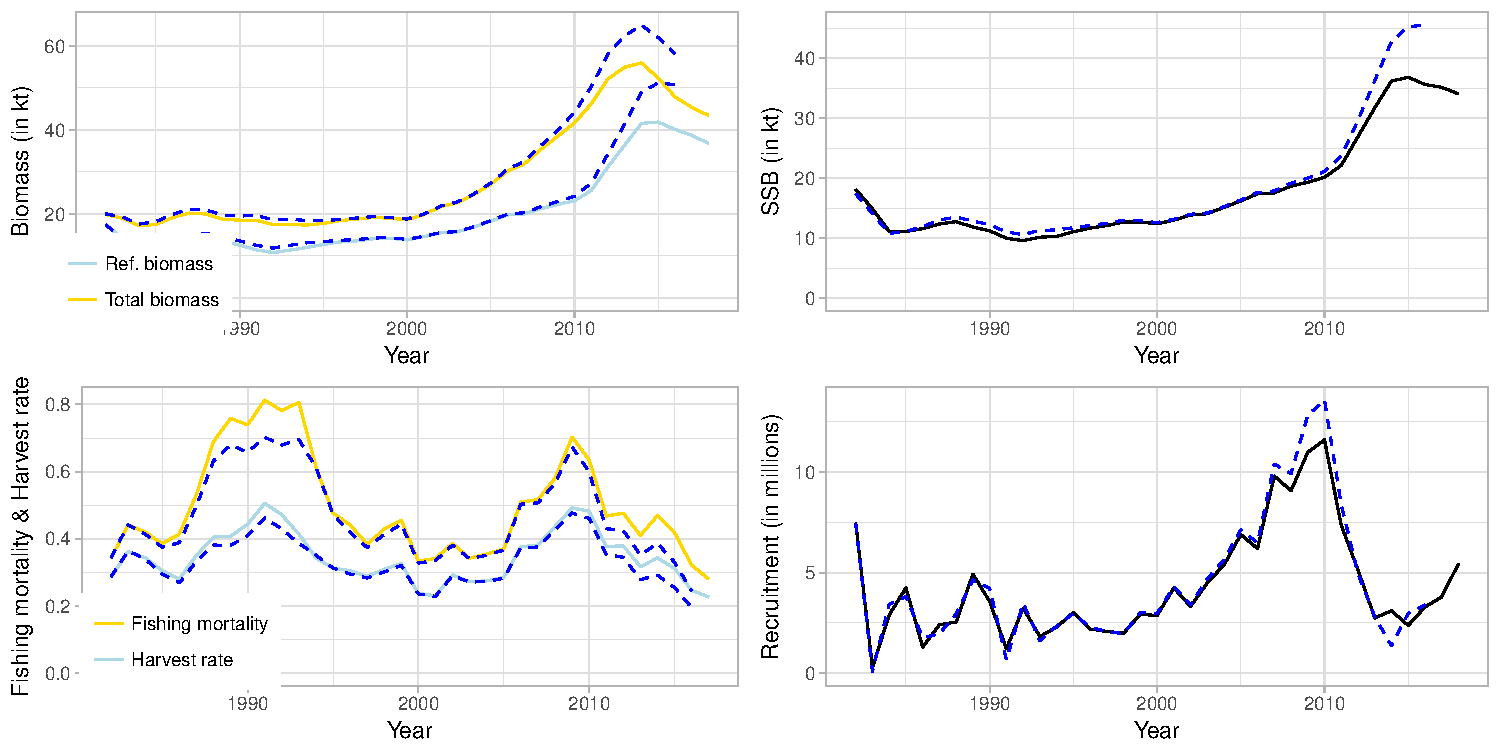
\includegraphics[width=\maxwidth]{figure/oldvsnew-1} 

\end{knitrout}
}

\frame{
\frametitle{Other derived quantities}

\begin{knitrout}
\definecolor{shadecolor}{rgb}{0.969, 0.969, 0.969}\color{fgcolor}
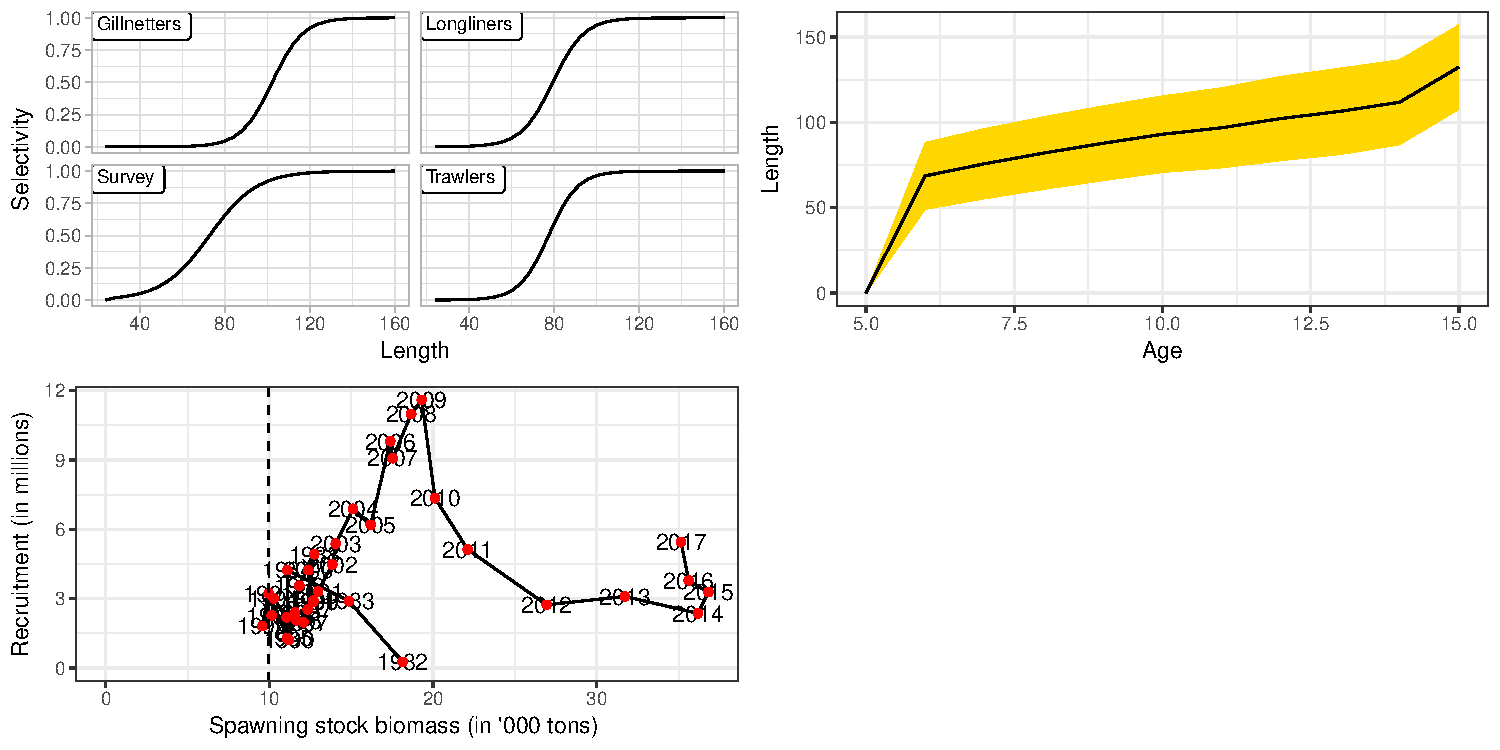
\includegraphics[width=\maxwidth]{figure/unnamed-chunk-15-1} 

\end{knitrout}


}



\frame{
\frametitle{Prognosis}


{\large
\textit{When the managment plan is applied, it is advised that no more than 6 074 tonnes ling are caught for the 2018/2019 fishing year.}
\par}

\begin{columns}
\begin{column}{0.5\linewidth}
\bi By calendar year
\ei

\begin{tabular}{r|r|r|r|r}
\hline
Year & HR & Catch & RefB & SSB\\
\hline
2016 & 0.268 & 9.88 & 37.30 & 35.85\\
\hline
2017 & 0.242 & 8.77 & 36.76 & 35.29\\
\hline
2018 & 0.257 & 8.79 & 34.75 & 34.20\\
\hline
2019 & 0.185 & 6.02 & 32.56 & 31.93\\
\hline
2020 & 0.179 & 5.86 & 32.58 & 31.91\\
\hline
2021 & 0.176 & 5.94 & 33.48 & 32.69\\
\hline
\end{tabular}


\end{column}
\begin{column}{0.5\linewidth}
\bi By fishing year
\ei

\begin{tabular}{l|r|r|r|r}
\hline
Year & HR & Catch & RefB & SSB\\
\hline
2015/2016 & 0.299 & 11.08 & 37.30 & 35.85\\
\hline
2016/2017 & 0.230 & 8.34 & 36.76 & 35.29\\
\hline
2017/2018 & 0.248 & 8.60 & 34.75 & 34.20\\
\hline
2018/2019 & 0.186 & 6.07 & 32.56 & 31.93\\
\hline
2019/2020 & 0.180 & 5.85 & 32.58 & 31.91\\
\hline
2020/2021 & 0.177 & 5.89 & 33.48 & 32.69\\
\hline
\end{tabular}


\end{column}
\end{columns}
}


\end{document}

% \frame{
% \frametitle{Location of samples}
% <<divisionplot,echo=FALSE,results='asis',fig.width=10, fig.height=5,cache=TRUE,warning=FALSE,message=FALSE>>=
% # tmp <-
% #   mfdb_dplyr_sample(mdb) %>%
% #   filter(species=='LIN',year==2015,data_source=='iceland-ldist') %>%
% #   left_join(mfdb_dplyr_division(mdb)) %>%
% #   left_join(mfdb:::mfdb_dplyr_table(mdb,'tow',"all_cols") %>%
% #               select(tow=name,tow_length=length,tow_depth=depth,
% #                      lat=latitude,lon=longitude)) %>%
% #   collect(n=Inf)
% # 
% # 
% # 
% # ## read mapping
% # 
% # reitmapping <-
% #   read.table(
% #         system.file("demo-data", "reitmapping.tsv", package="mfdb"),
% #         header=TRUE,
% #         as.is=TRUE) %>%
% #   dplyr::mutate(sr=as.numeric(GRIDCELL)) %>%
% #   mar:::sr2d() %>%
% #   filter(SUBDIVISION %in% tmp$division)
% # 
% # 
% # 
% # test <-
% #   plyr::ddply(reitmapping, 'SUBDIVISION',
% #         function(x){
% #           ##   2
% #           ## 1 x 3
% #           ##   4
% #           sides <- rep(10*x$GRIDCELL,each=4) + 1:4
% #           up <- geo::d2sr(x$lat + 0.125, x$lon)
% #           down <- geo::d2sr(x$lat - 0.126, x$lon)
% #           left <- geo::d2sr(x$lat, x$lon - 0.25)
% #           right <- geo::d2sr(x$lat, x$lon + 0.26)
% # 
% #           for(i in 1:nrow(x)){
% #             ## up
% #             if(up[i] %in% x$GRIDCELL){
% #               sides[4*(i-1)+2] <- NA
% #               sides[sides==(10*up[i]+4)] <- NA
% #             }
% #             ## down
% #             if(down[i] %in% x$GRIDCELL){
% #               sides[4*(i-1)+4] <- NA
% #               sides[sides==(10*down[i]+2)] <- NA
% #             }
% #             ## left
% #             if(left[i] %in% x$GRIDCELL){
% #               sides[4*(i-1)+1] <- NA
% #               sides[sides==(10*left[i]+3)] <- NA
% #             }
% #             ## right
% #             if(right[i] %in% x$GRIDCELL){
% #               sides[4*(i-1)+3] <- NA
% #               sides[sides==(10*right[i]+1)] <- NA
% #             }
% #           }
% #           sides <- sides[!is.na(sides)]
% #           corners <- plyr::ddply(data.frame(side=rep(sides,each=2)),
% #                        'side',
% #                        function(x){
% #                          loc <- geo::sr2d(floor(x$side[1]/10))
% #                          loc <- c(loc$lat,loc$lon)
% #                          if((x$side[1] %% 10) == 1){
% #                            up.loc <- loc+c(0.125,-0.25)
% #                            down.loc <- loc+c(-0.125,-0.25)
% #                          }
% #                          if((x$side[1] %% 10) == 3){
% #                            up.loc <- loc+c(0.125,0.25)
% #                            down.loc <- loc+c(-0.125,0.25)
% #                          }
% #                          if((x$side[1] %% 10) == 2){
% #                            up.loc <- loc+c(0.125,-0.25)
% #                            down.loc <- loc+c(0.125,0.25)
% #                          }
% #                          if((x$side[1] %% 10) == 4){
% #                            up.loc <- loc+c(-0.125,-0.25)
% #                            down.loc <- loc+c(-0.125,0.25)
% #                          }
% #                          tmp <- as.data.frame(rbind(up.loc,down.loc))
% #                          names(tmp) <- c('lat','lon')
% #                          return(tmp)
% #                        })
% #           corners$order <- NA
% #           corners$order[1:2] <- 1:2
% #           counter <- 1:nrow(corners)
% #           i <- 2
% #           for(order in 3:(length(sides))){
% #             tmp <- counter[is.na(corners$order) &
% #                            corners$lat == corners$lat[i] &
% #                            corners$lon == corners$lon[i]][1]
% #             corners$order[corners$side == corners$side[tmp]] <- order
% #             corners <- corners[-tmp,]
% #             i <- which(corners$order == order)
% # 
% #           }
% #           corners$side <- NULL
% #           return(arrange(corners,order))
% # 
% #         })
% # 
% # bcareas <- c(1015, 1014, 1018, 1011, 1012, 1023, 1023, 1021, 1032, 1031,
% #              1042, 1041, 1052, 1053, 1051, 1054, 1061, 1071, 1081, 1082)
% # 
% # 
% #  ggplot(data.frame(lat=0,lon=0), aes(lon,lat)) +
% # #  ggplot(subset(dat,ar==2011),aes(lon,lat)) +
% # #  stat_density2d(aes(fill=..level..),geom='polygon') +
% # #  scale_fill_gradient(limits = c(0,0.2), low='yellow',high='red') +
% #   geom_point(col='yellow') +
% #   geom_path(data=geo::gbdypi.100,lty=2,size = 0.3) +
% #   geom_path(data=geo::gbdypi.800,lty=2,size = 0.3) +
% #   #  geom_polygon(alpha=0.5,data=geo::gbdypi.100,fill='gray90') +
% #   geom_path(data=geo::gbdypi.200,lty=2,size = 0.3) + #alpha=0.5,fill='gray90',
% #   geom_path(data=geo::gbdypi.500,lty=3,size = 0.3) +
% #   geom_path(data=geo::gbdypi.1000,lty=4,size = 0.3) +
% #   geom_path(aes(lon,lat,group=SUBDIVISION),
% #             data=test, #
% #             #subset(test,SUBDIVISION %in% bcareas),
% #             size = 0.3) +
% # 
% # 
% #   geom_polygon(data=geo::island, col = 'black' ,fill = 'gray70',size = 0.3) +
% # #  geom_polygon(data=geo::greenland, col = 'black', fill = 'gray70') +
% #   geom_polygon(data=geo::eyjar, col = 'black', fill = 'gray70',size = 0.3) +
% #   geom_polygon(data=geo::faeroes, col = 'black', fill = 'gray70') +
% #   coord_map('mercator', xlim=c(-30,-10),ylim=c(62,68)) +
% # #     geom_label(aes(lon,lat,label=SUBDIVISION),
% # #            data=ddply(test,~SUBDIVISION, summarise, lat=mean(lat),
% # #              lon=mean(lon))) +
% # #  coord_map('mercator', xlim=c(-28,-9.5),ylim=c(62.5,68)) +
% #   xlab('Longitude') +
% #   ylab('Latitude') +
% #   theme_light() +
% #   geom_point(data=tmp %>% select(tow,lat,lon) %>% distinct()) +
% #   geom_path(data = geo::twohmiles, lty = 2) #+
% # #  geom_path(data=icelandrivers,size=0.1,col='blue') +
% # #  geom_path(data=glaciers,size=0.5)
% 
% sampling_pos_plot
% 
% @
% 
% }
% 
% 
% 
% \frame{
% \frametitle{Landings data}
% 
% \begin{columns}
% \begin{column}{0.5\linewidth}
% Sources of landings data:
% \bi Landings of Icelandic vessels:
%   \bi Pre 1993: landings by port from Fiskifélagið
%   \item Post 1993: Directorate of fisheries, catches reported by vessel
%   \ei
% \item Landings of foreign vessels:
%   \bi Pre 2014: Statlant
%   \item Post 2014: Directorate of fisheries, catches reported by vessel
%   \ei
% \ei
% 
% \end{column}
% \begin{column}{0.5\linewidth}
% <<echo=FALSE,cache=TRUE>>=
% fit$fleet.info %>%
%   filter(fleet !='igfs', year < thisyear) %>%
%   ggplot(aes(year,amount/1e6,fill=fleet)) + geom_bar(stat='identity') +
%   theme_light() +
%   labs(y='Landed catch (kt)',x='Year') +
%   theme(legend.position = c(0.1,0.8))
% @
% \end{column}
% \end{columns}
% }
% 
% 
% 
% \frame{
% \frametitle{Available samples}
% <<echo=FALSE,results='asis',fig.width=10, fig.height=5,cache=TRUE,message=FALSE,warning=FALSE>>=
%  mfdb_dplyr_sample(mdb) %>%
%   filter(year %in% 1982:2017,
%          sampling_type %in% c('IGFS','SEA'),
%          data_source %in% c('iceland-ldist','iceland-aldist'),
%          species == 'LIN',
%           !is.na(age)) %>%
%   mutate(sampling_type = ifelse(sampling_type=='IGFS','Survey', 'Commercial'),
%          data_source = ifelse(data_source == 'iceland-aldist','Age','Length')) %>%
%   group_by(sampling_type,year,data_source) %>%
%   dplyr::summarise(ntow=n_distinct(tow)) %>%
%   collect(n=Inf) %>%
%   ungroup() %>%
%   tidyr::spread(data_source,ntow,fill = 0) %>%
%   mutate(Age = ifelse(year > 1999, Age, 0),
%          Length = abs(Length - Age)) %>%
%   tidyr::gather(col,n,-c(year,sampling_type)) %>%
%   mutate(col = ifelse(col == 'Age','Age & length','Only Length')) %>%
%    ggplot(aes(year,n,fill = col)) + geom_bar(stat='identity') + #,fill='#0076a9') +
%    facet_wrap(~sampling_type,scale='free_y')+
%    theme_light() +
%      geom_label(data= data_frame(sampling_type=c('Survey','Commercial'),
%                                  label=c('Survey','Commercial')),
%             aes(label=label,group=1),x=-Inf,y=Inf,size=3, vjust = 1,hjust=-0.1,fill='white') +
%   theme(strip.background = element_blank(),strip.text=element_text(size = 0),
%         legend.position = c(0.1,0.5),
%         legend.background =  element_rect(fill = "transparent",colour = NA)) +
%   labs(y='',x='Year',fill='')
% 
% 
% @
% 
% }
% 
% 
% 
% %\section{Data available}
% \begin{frame}
% \frametitle{Landings and discards}
% 
% Landings
% \begin{itemize}
%   \item Landings from Icelandic vessels given by the Directorate of
%     Fisheries
%   \item Landings by Norwegian and Faroese vessels given by the
%     Icelandic Coast Guard
%     \item Landings from XIVb given by STATLANT
% \end{itemize}
% 
% Discards
% \begin{itemize}
%   \item Estimated low (<1\% in either numbers or weight), WGDEEP2011:WD02
%   \item No estimates from XIVb
% \end{itemize}
% \end{frame}
% 
% \frame{
% \frametitle{Depth distribution of commercial catches}
% <<depthplot,echo=FALSE,results='asis',fig.width=10, fig.height=5,cache=TRUE,warning=FALSE,message=FALSE>>=
% library(Logbooks)
% bv<-botnv[botnv$langa>0 & botnv$ar>1999,]
% li<-lina[lina$langa>0 & lina$ar>1999,]
% ne<-net[net$langa>0 & net$ar>1999,]
% bv$d<-round(bv$dypi/50)*50
% li$d<-round(li$dypi/50)*50
% ne$d<-round(ne$dypi/50)*50
% 
% par(mfcol=c(3,4),oma=c(4,5,1,1), mar=c(1,1,0,0))
% 
% year_ser<-c(2003,2010,2015,lastyear)
% 
% for(i in year_ser){
%   lina.d<-tapply(li$langa[li$ar==i], li$d[li$ar==i], sum)
%   botnv.d<-tapply(bv$langa[bv$ar==i], bv$d[bv$ar==i], sum)
%   net.d<-tapply(ne$langa[ne$ar==i], ne$d[ne$ar==i], sum)
%   barplot(names.arg=as.numeric(names(lina.d)), height = lina.d/sum(lina.d), col = 'turquoise2', ylim = c(0, 0.52), xlim = c(0, 1000/50), xaxt = 'n', yaxt = 'n')
%   mtext(i, line = -1)
%   if(i == year_ser[1]){axis(2, labels=T, at=seq(0,0.5,0.1), mgp=c(0,0.2,0), cex=1.2, tck=0.02, adj=1, las=1)}
%   text(900,0.3, i, cex=1.5, adj=1)
%   if(i==year_ser[1]){mtext(side=2, "Longlines",outer=T, line=1.8, cex=1, adj=0.95)}
%   text(900,0.4, i, cex=1.5, adj=1)
%   barplot(names.arg=as.numeric(names(botnv.d)), height = botnv.d/sum(botnv.d), col = 'turquoise2', ylim = c(0, 0.52), xlim = c(0, 1000/50), xaxt = 'n', yaxt = 'n')
%   if(i == year_ser[1]){axis(2, labels=T, at=seq(0,0.5,0.1), mgp=c(0,0.2,0), cex.axis=1.2, tck=0.02, adj=1, las=1)}
%    if(i==year_ser[1]){mtext(side=2, "Trawls",outer=T, line=1.8, cex=1, adj=0.5)}
%   text(900,0.3, i, cex=1.5, adj=1)
%   barplot(names.arg=as.numeric(names(net.d)), height = net.d/sum(net.d), col = 'turquoise2', ylim = c(0, 0.52), xlim = c(0, 1000/50), xaxt = 'n', yaxt = 'n')
%   axis(1, labels=c(0,250,500,750,1000), at=c(0,250,500,750,1000)/50, mgp=c(0,0.2,0), cex.axis=1.2, tck=0.02)
%   if(i == year_ser[1]){axis(2, labels=T, at=seq(0,0.5,0.1), mgp=c(0,0.2,0), cex.axis=1.2, tck=0.02, adj=1, las=1)}
%    if(i==year_ser[1]){mtext(side=2, "Gillnets",outer=T, line=1.8, cex=1, adj=0.1)}
% }
% mtext(side=1,'Depth (m)', outer=TRUE, line=1, cex=1)
% @
% 
% }
% 
% \frame{
% \frametitle{Gadget length- and age-based model settings}
% \bi Two stock model: immature and mature
% \bi Age: 3--10 and 5--15
% \item Length: 20--160 cm, $\Delta l$ 4 cm
% \item Length based maturation function
% \item Natural mortality set to be 0.15 for all years
% \item Length based Von Bertalanffy growth
% \item Annual recruitment of 3 year olds
% \ei
% \item Five fleets: survey, longlines, bottom trawlers, gillnets and foreign vessels
% \item Model time: 1982--2017, quarterly timestep
% \item A total of 71 parameters estimated
% \ei
% 
% }

% \frame{
% \frametitle{Fleet selection}
% <<echo=FALSE,results='asis',fig.width=5, fig.height=3,cache=TRUE,warning=FALSE,message=FALSE>>=
% fit$suitability %>%
%   #filter(!(model %in% c(22,70,73,24,56,64)))%>%
%     filter(year == 2000,step == 2) %>% 
%   #ggplot(aes(length, suit,lty = fleet)) +
%   #  geom_line()
%   filter(fleet != 'foreign',grepl('mat',stock)) %>%
%   ungroup() %>% 
%   mutate(fleet = ifelse(fleet=='igfs','Survey',
%                         ifelse(fleet=='lln','Longliners',
%                                ifelse(fleet == 'gil','Gillnetters','Trawlers'))))%>%
% #  group_by(fleet,length) %>%
% #  summarise(ms=median(suit), #this is now median among year x step combos,
% #            us=quantile(suit,0.975), #quantiles not really useful 
% #            ls=quantile(suit,0.025)) %>%
% #  ggplot(aes(length,ms)) +
%   ggplot(aes(length,suit)) +
% #  geom_line(aes(length,suit),fit$suitability %>% filter(fleet != 'foreign',grepl('mat',stock)) %>%
% #  ungroup() %>% 
% #  mutate(fleet = ifelse(fleet=='igfs','Survey',
% #                        ifelse(fleet=='lln','Longliners',
% #                               ifelse(fleet == 'gil','Gilnetters','Trawlers')))) ,col='red') +
%   #geom_ribbon(aes(ymax=us,ymin=ls),fill='gold',alpha=0.5) + 
%   geom_line() +
%   theme_light() +
%   facet_wrap(~fleet) +
%   labs(y='Suitability',x='Length') +
%   theme(legend.position =c(0.8,0.2),
%         legend.background = element_blank(),
%         strip.background = element_blank(),
%         strip.text = element_blank()) +
%   geom_label(data=data.frame(fleet = c('Survey','Longliners','Gillnetters','Trawlers')),
%              aes(label=fleet),x=-Inf,y=Inf,size=3, vjust = 1,hjust=-0.)
% @
% 
% }
% 
% \frame{
% \frametitle{SSB-Rec relationship}
% <<echo=FALSE,results='asis',fig.width=10, fig.height=5,cache=TRUE,warning=FALSE,message=FALSE>>=
% bloss_old_def <-
%   fit$res.by.year %>%
%   filter(grepl('mat',stock)) %>%
%   select(total.biomass) %>% 
%   min(.)/1e6
%   #group_by(model) %>%
%   #dplyr::summarise(bloss=min(total.biomass)/1e6)#this is likely not the same! So needs to be defined manually
% 
% 
% 
% tmp <-
% fit$res.by.year %>%
%   group_by(year) %>%
%   #group_by(year,model) %>%
%   dplyr::summarise(recruitment=sum(recruitment,na.rm=TRUE)/1e6,
%                    ssb = total.biomass[grepl('mat',stock)]/1e6) %>%
%   ungroup()
% tmp %>%
%   left_join(tmp %>%
% #              select(model,year,ssb.5=ssb) %>%
%               select(year,ssb.5=ssb) %>%
%               dplyr::mutate(year=year+1)) %>%
%   group_by(year) %>%
%   dplyr::summarise(mr=median(recruitment),
%             ur=quantile(recruitment,0.975),
%             lr=quantile(recruitment,0.025),
%             ms=median(ssb.5,na.rm=TRUE),
%             us=quantile(ssb.5,0.975,na.rm=TRUE),
%             ls=quantile(ssb.5,0.025,na.rm=TRUE)) %>% #just 1 value so medians=quantiles
%   ggplot(aes(ms,mr)) +
% 
% #    geom_rect(ymin=-Inf,ymax=Inf,xmin=quantile(bloss$bloss,0.975),
% #              xmax=quantile(bloss$bloss,0.025),fill='gold')+
% #    geom_vline(xintercept = median(bloss$bloss),lty=2)+
%     geom_vline(xintercept = bloss,lty=2)+
%     # geom_vline(xintercept = fit$res.by.year %>%
%     #              filter(grepl('mat',stock)) %>%
%     #              ungroup() %>%
%     #              dplyr::summarise(min(total.biomass)/1e6) %>%
%     #              unlist(),col='red')+
% #    geom_errorbar(aes(ymax=ur,ymin=lr),col='grey') +
% #    geom_errorbarh(aes(xmax=us,xmin=ls),col='grey') +
%     geom_path()+
%     geom_point(col='red')+
%     geom_text(aes(label=year-1),vjust=0.15,hjust=0.15) +
%    xlab('Spawning stock biomass (in \'000 tons) ') +
%   ylab('Recruitment (in millions)') + theme_light() +
%   expand_limits(x=0,y=0)
% 
% @
% 
% }
% 

% \frame{
% \frametitle{Available samples on length}
% 
%  <<echo=FALSE,results='asis',fig.width=10, fig.height=5,message=FALSE,warning=FALSE>>=
%  mfdb_dplyr_sample(mdb) %>%
%    filter(year %in% 1982:lastyear,
%           sampling_type %in% c('IGFS','SEA'),
%           data_source =='iceland-ldist',
%           species == 'LIN') %>%
%    mutate(sampling_type = ifelse(sampling_type=='IGFS','igfs',
%                                         ifelse(gear %in%  c('LLN','HLN'), 'lln',
%                                                ifelse(gear %in% c('BMT','NPT','DSE','PSE','PGT','SHT'),'bmt','gil')))) %>%
%    group_by(sampling_type,year) %>%
%    dplyr::summarise(ntow=n_distinct(tow),n=sum(count)) %>%
%    collect(n=Inf) %>%
%    ungroup() %>%
%    tidyr::gather(col,n,-c(year,sampling_type)) %>%
%    ggplot(aes(year,n)) + geom_bar(stat='identity',fill='#0076a9') +
%    facet_wrap(~col+sampling_type,scale='free_y',ncol=4)+
%    theme_light() +
%      geom_label(data= data_frame(col=rep(c('n','ntow'),4),
%                                  sampling_type=rep(c('lln','bmt','gil','igfs'),each=2),
%                                  label=c('Longline \n (n measured)','Longline\n (n tows)',
%                                          'Bottom trawl \n (n measured)','Bottom trawl\n (n tows)',
%                                          'Gilnet \n (n measured)','Gilnet\n (n tows)',
%                                          'Survey\n (n measured)','Survey\n (n tows)')),
%             aes(label=label,group=1),x=-Inf,y=Inf,size=3, vjust = 1,hjust=-0.1) +
%   theme(strip.background = element_blank(),strip.text=element_text(size = 0)) +
%   labs(y='Num. samples/tow',x='Year')
% 
% 
% # fit$catchdist.fleets %>%
% #   filter(name %in% c('aldist.igfs','ldist.igfs')) %>%
% #   group_by(name,year) %>%
% #   dplyr::summarise(n=sum(number.x,na.rm=TRUE)) %>%
% #   bind_rows(fit$stockdist %>%
% #               as.data.frame() %>%
% #               select(year,name,number.x) %>%
% #               group_by(year,name) %>%
% #               dplyr::summarise(n=sum(number.x,na.rm=TRUE))) %>%
% #   ggplot(aes(year,n)) + geom_bar(stat = 'identity',fill='#0076a9') + facet_wrap(~name,ncol=1,scale='free_y') +
% #   theme_minimal() +
% #   labs(y='Num. samples',x='Year')
% @
% }
% 
% % \frame{
% \frametitle{Recruitment parameters}
% <<echo=FALSE,results='asis',fig.width=10, fig.height=5,cache=TRUE,warning=FALSE,message=FALSE>>=
% fit$res.by.year %>%
%   #filter(!(model %in% c(22,70,73,24,56,64))) %>%
%   filter(grepl('imm',stock)) %>%
%   dplyr::mutate(recruitment = recruitment/1e6) %>%
%   ggplot(aes(year,recruitment,group=round(year))) + 
%    geom_point()+#geom_ribbon(aes(ymin=l,ymax=u),fill="gold") + geom_line() +
%   geom_line(data=fit$res.by.year %>% filter(grepl('imm',stock)),
%             aes(y=recruitment/1e6,group=stock),col='red') +
%   labs(y='Recruitment (in millions)',x='Year') +
%   theme_light()
% @
% }
% 
% 
% \frame{
% \frametitle{Survey catchability}
% <<echo=FALSE,results='asis',fig.width=10, fig.height=5,cache=TRUE,warning=FALSE,message=FALSE>>=
% fit$sidat %>%
% #  select(model,name,intercept) %>%
%   select(name,intercept) %>%
%   distinct() %>%
%   ggplot(aes(name,exp(intercept))) + geom_point() +
%   geom_line(aes(group=1),col='red',
%             data=fit$sidat %>%
%               select(name,intercept) %>%
%               distinct()) +
%   theme_light() +
%   labs(x='Survey index',y=expression(q[g]))
% @
% 
% }
% \frame{
% \frametitle{Summary of reference points}
% \bi The managment rule takes the form of $C_y = H B_{75cm^+}$
% \item Last year a management strategy evaluation was performed to set H based on the following reference points.
% \item No evidence of impaired recruitment and fishing mortality is considered to have been low
% \item $B_{loss} = 9.93 kt$ (min SSB of the time series) was set to for $B_{pa}$
% \item $B_{lim} = B_{pa}/1.4 = 7.09$
% \item $H_{lim}$ determined as the harvest rate that has 50\% chance of SSB being at $B_{lim}$ via stochastic simulation without assessment error
% \item Variability in recruitment is based on a block bootstrap of estimated recruitment, block size of 6 consecutive years.
% \item $F_{lim}$, $F_{pa}$ and $H_{pa}$ were based on the estimate of $H_{lim}$
% \item $H_{msy}$ was based on simulation with assessment error (lognormal with $\rho = 0.8$, and $\sigma$ as the CV of $B_{75cm^+}$)
% \ei
% }
% 

% 
% \frame{
% \frametitle{Available samples on length}
% 
%  <<echo=FALSE,results='asis',fig.width=10, fig.height=5,message=FALSE,warning=FALSE>>=
%  mfdb_dplyr_sample(mdb) %>%
%    filter(year %in% 1982:lastyear,
%           sampling_type %in% c('IGFS','SEA'),
%           data_source =='iceland-ldist',
%           species == 'LIN') %>%
%    mutate(sampling_type = ifelse(sampling_type=='IGFS','igfs',
%                                         ifelse(gear %in%  c('LLN','HLN'), 'lln',
%                                                ifelse(gear %in% c('BMT','NPT','DSE','PSE','PGT','SHT'),'bmt','gil')))) %>%
%    group_by(sampling_type,year) %>%
%    dplyr::summarise(ntow=n_distinct(tow),n=sum(count)) %>%
%    collect(n=Inf) %>%
%    ungroup() %>%
%    tidyr::gather(col,n,-c(year,sampling_type)) %>%
%    ggplot(aes(year,n)) + geom_bar(stat='identity',fill='#0076a9') +
%    facet_wrap(~col+sampling_type,scale='free_y',ncol=4)+
%    theme_light() +
%      geom_label(data= data_frame(col=rep(c('n','ntow'),4),
%                                  sampling_type=rep(c('lln','bmt','gil','igfs'),each=2),
%                                  label=c('Longline \n (n measured)','Longline\n (n tows)',
%                                          'Bottom trawl \n (n measured)','Bottom trawl\n (n tows)',
%                                          'Gilnet \n (n measured)','Gilnet\n (n tows)',
%                                          'Survey\n (n measured)','Survey\n (n tows)')),
%             aes(label=label,group=1),x=-Inf,y=Inf,size=3, vjust = 1,hjust=-0.1) +
%   theme(strip.background = element_blank(),strip.text=element_text(size = 0)) +
%   labs(y='Num. samples/tow',x='Year')
% 
% 
% # fit$catchdist.fleets %>%
% #   filter(name %in% c('aldist.igfs','ldist.igfs')) %>%
% #   group_by(name,year) %>%
% #   dplyr::summarise(n=sum(number.x,na.rm=TRUE)) %>%
% #   bind_rows(fit$stockdist %>%
% #               as.data.frame() %>%
% #               select(year,name,number.x) %>%
% #               group_by(year,name) %>%
% #               dplyr::summarise(n=sum(number.x,na.rm=TRUE))) %>%
% #   ggplot(aes(year,n)) + geom_bar(stat = 'identity',fill='#0076a9') + facet_wrap(~name,ncol=1,scale='free_y') +
% #   theme_minimal() +
% #   labs(y='Num. samples',x='Year')
% @
% }

% \begin{frame}
% \frametitle{Survey indices}
% \begin{columns}
% \begin{column}{0.3\linewidth}
% \begin{table}[!h]
% {\centering \tiny
% \scriptsize
% \begin{tabular}{l r r}
% \toprule
% Name& min& max \\ \midrule
% <<echo=FALSE,results='asis',cache=TRUE>>=
% fit$sidat %>%
%    group_by(name) %>%
%    summarise(min=min(lower),
%              max=max(upper)) %>%
%    unite(col,matches("."),sep=' & ') %>%
%    (function(x){
%      paste(x$col,collapse = '\\\\ \n')
%    }) %>%
%    paste0('\\\\') %>%
%    cat()
% @
% 
% \bottomrule
% \end{tabular}
% \par}
% \end{table}
% 
% \end{column}
% \begin{column}{0.7\linewidth}
% <<echo=FALSE,results='asis',fig.width=10, fig.height=5,cache=TRUE,warning=FALSE,message=FALSE>>=
% fit$catchdist.fleets %>%
%    filter(name=='ldist.igfs',year %in% 2010:2013) %>%
%    ungroup() %>% 
%    ggplot(aes(lower,number.x))+
%    geom_rect(fill='gold',alpha=0.01,xmin=20,xmax=52,ymin=-Inf,ymax=Inf)+
%    geom_rect(fill='gold',alpha=0.01,xmin=60,xmax=72,ymin=-Inf,ymax=Inf)+
%    geom_rect(fill='gold',alpha=0.01,xmin=80,xmax=92,ymin=-Inf,ymax=Inf)+
%    geom_rect(fill='gold',alpha=0.01,xmin=100,xmax=160,ymin=-Inf,ymax=Inf)+
%    geom_line() + facet_wrap(~year) + xlim(c(20,120)) +
%    theme_light() + labs(x='Length', y='Number observed') +
%    geom_label(data=data_frame(year=2010:2013),
%               aes(label=year,group=1),x=-Inf,y=Inf,size=3, vjust = 1.1,hjust=-0.1) +
%    theme(strip.background = element_blank(),strip.text = element_text(size = 0))
% @
% \end{column}
% \end{columns}
% \end{frame}

%\begin{frame}
% \frametitle{Spatial distribution of ling catches in Va (Longline) - figure needs updating}
%  {\centering
% 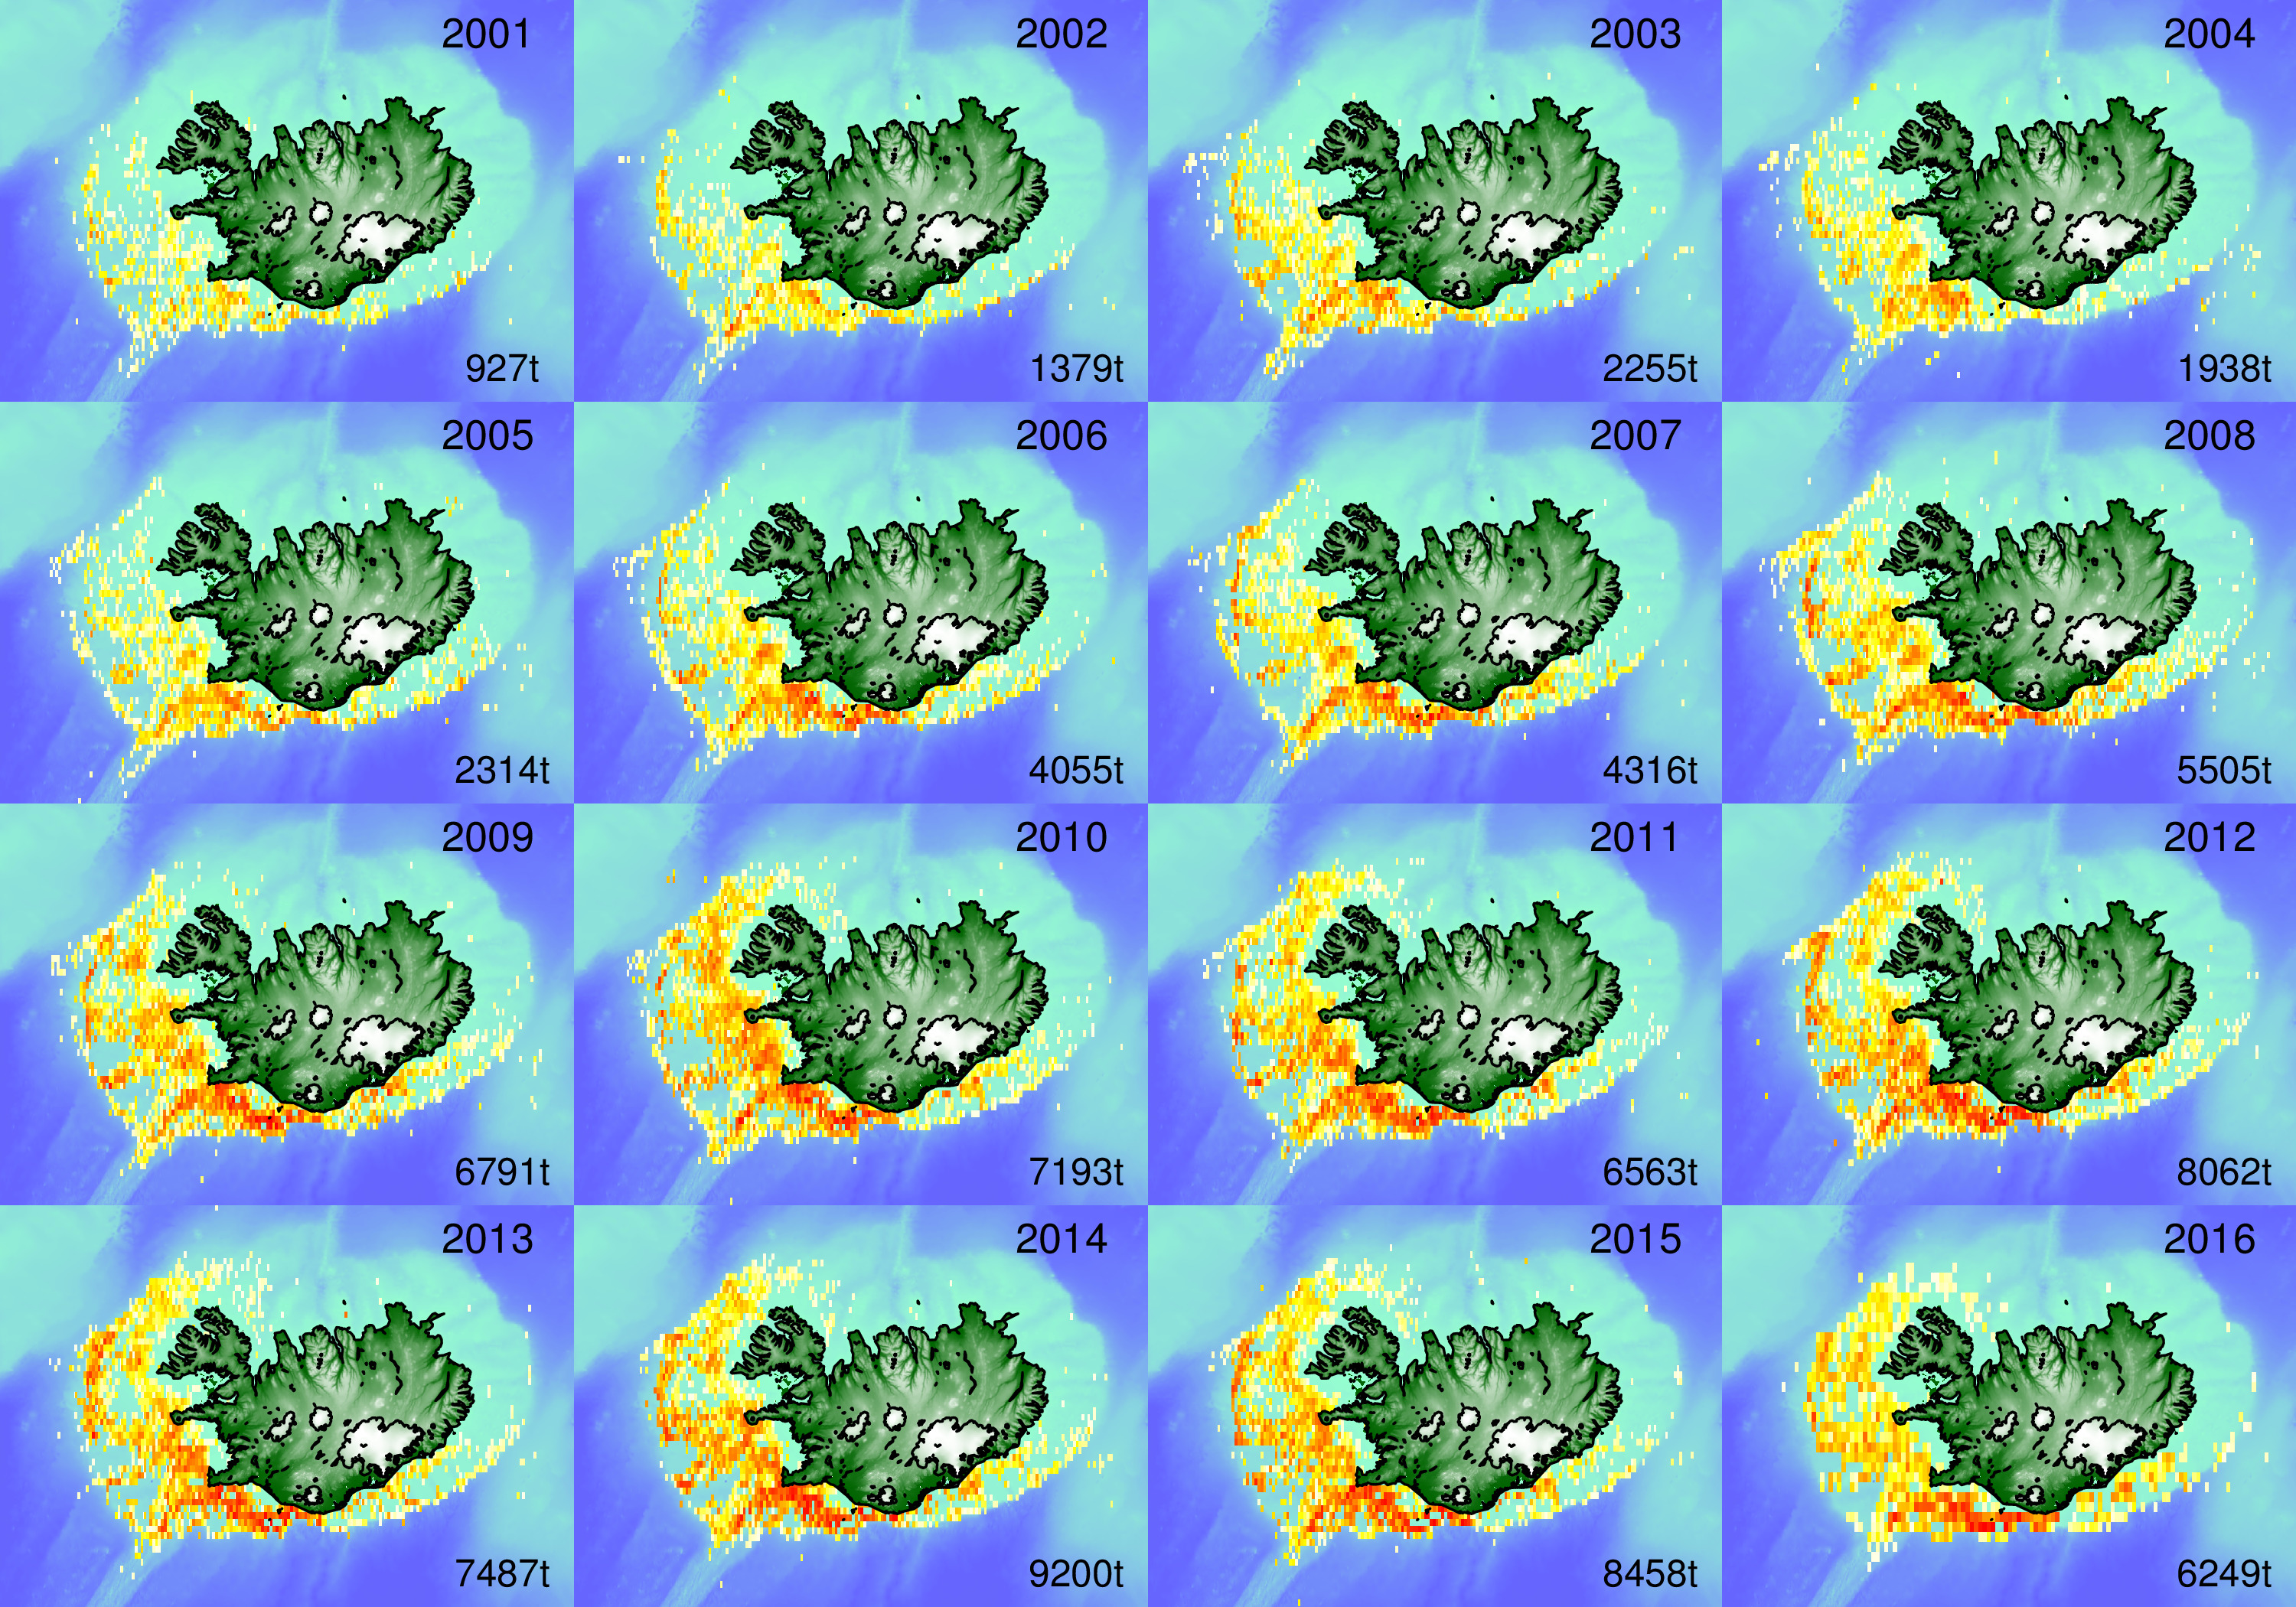
\includegraphics[width=0.7\linewidth, angle=0]{SpatialMapLogb.jpg}
% \par}
% \end{frame}
% 
% \begin{frame}
% \frametitle{Spatial distribution of ling catches in Va - figure needs updating}
%  {\centering
% 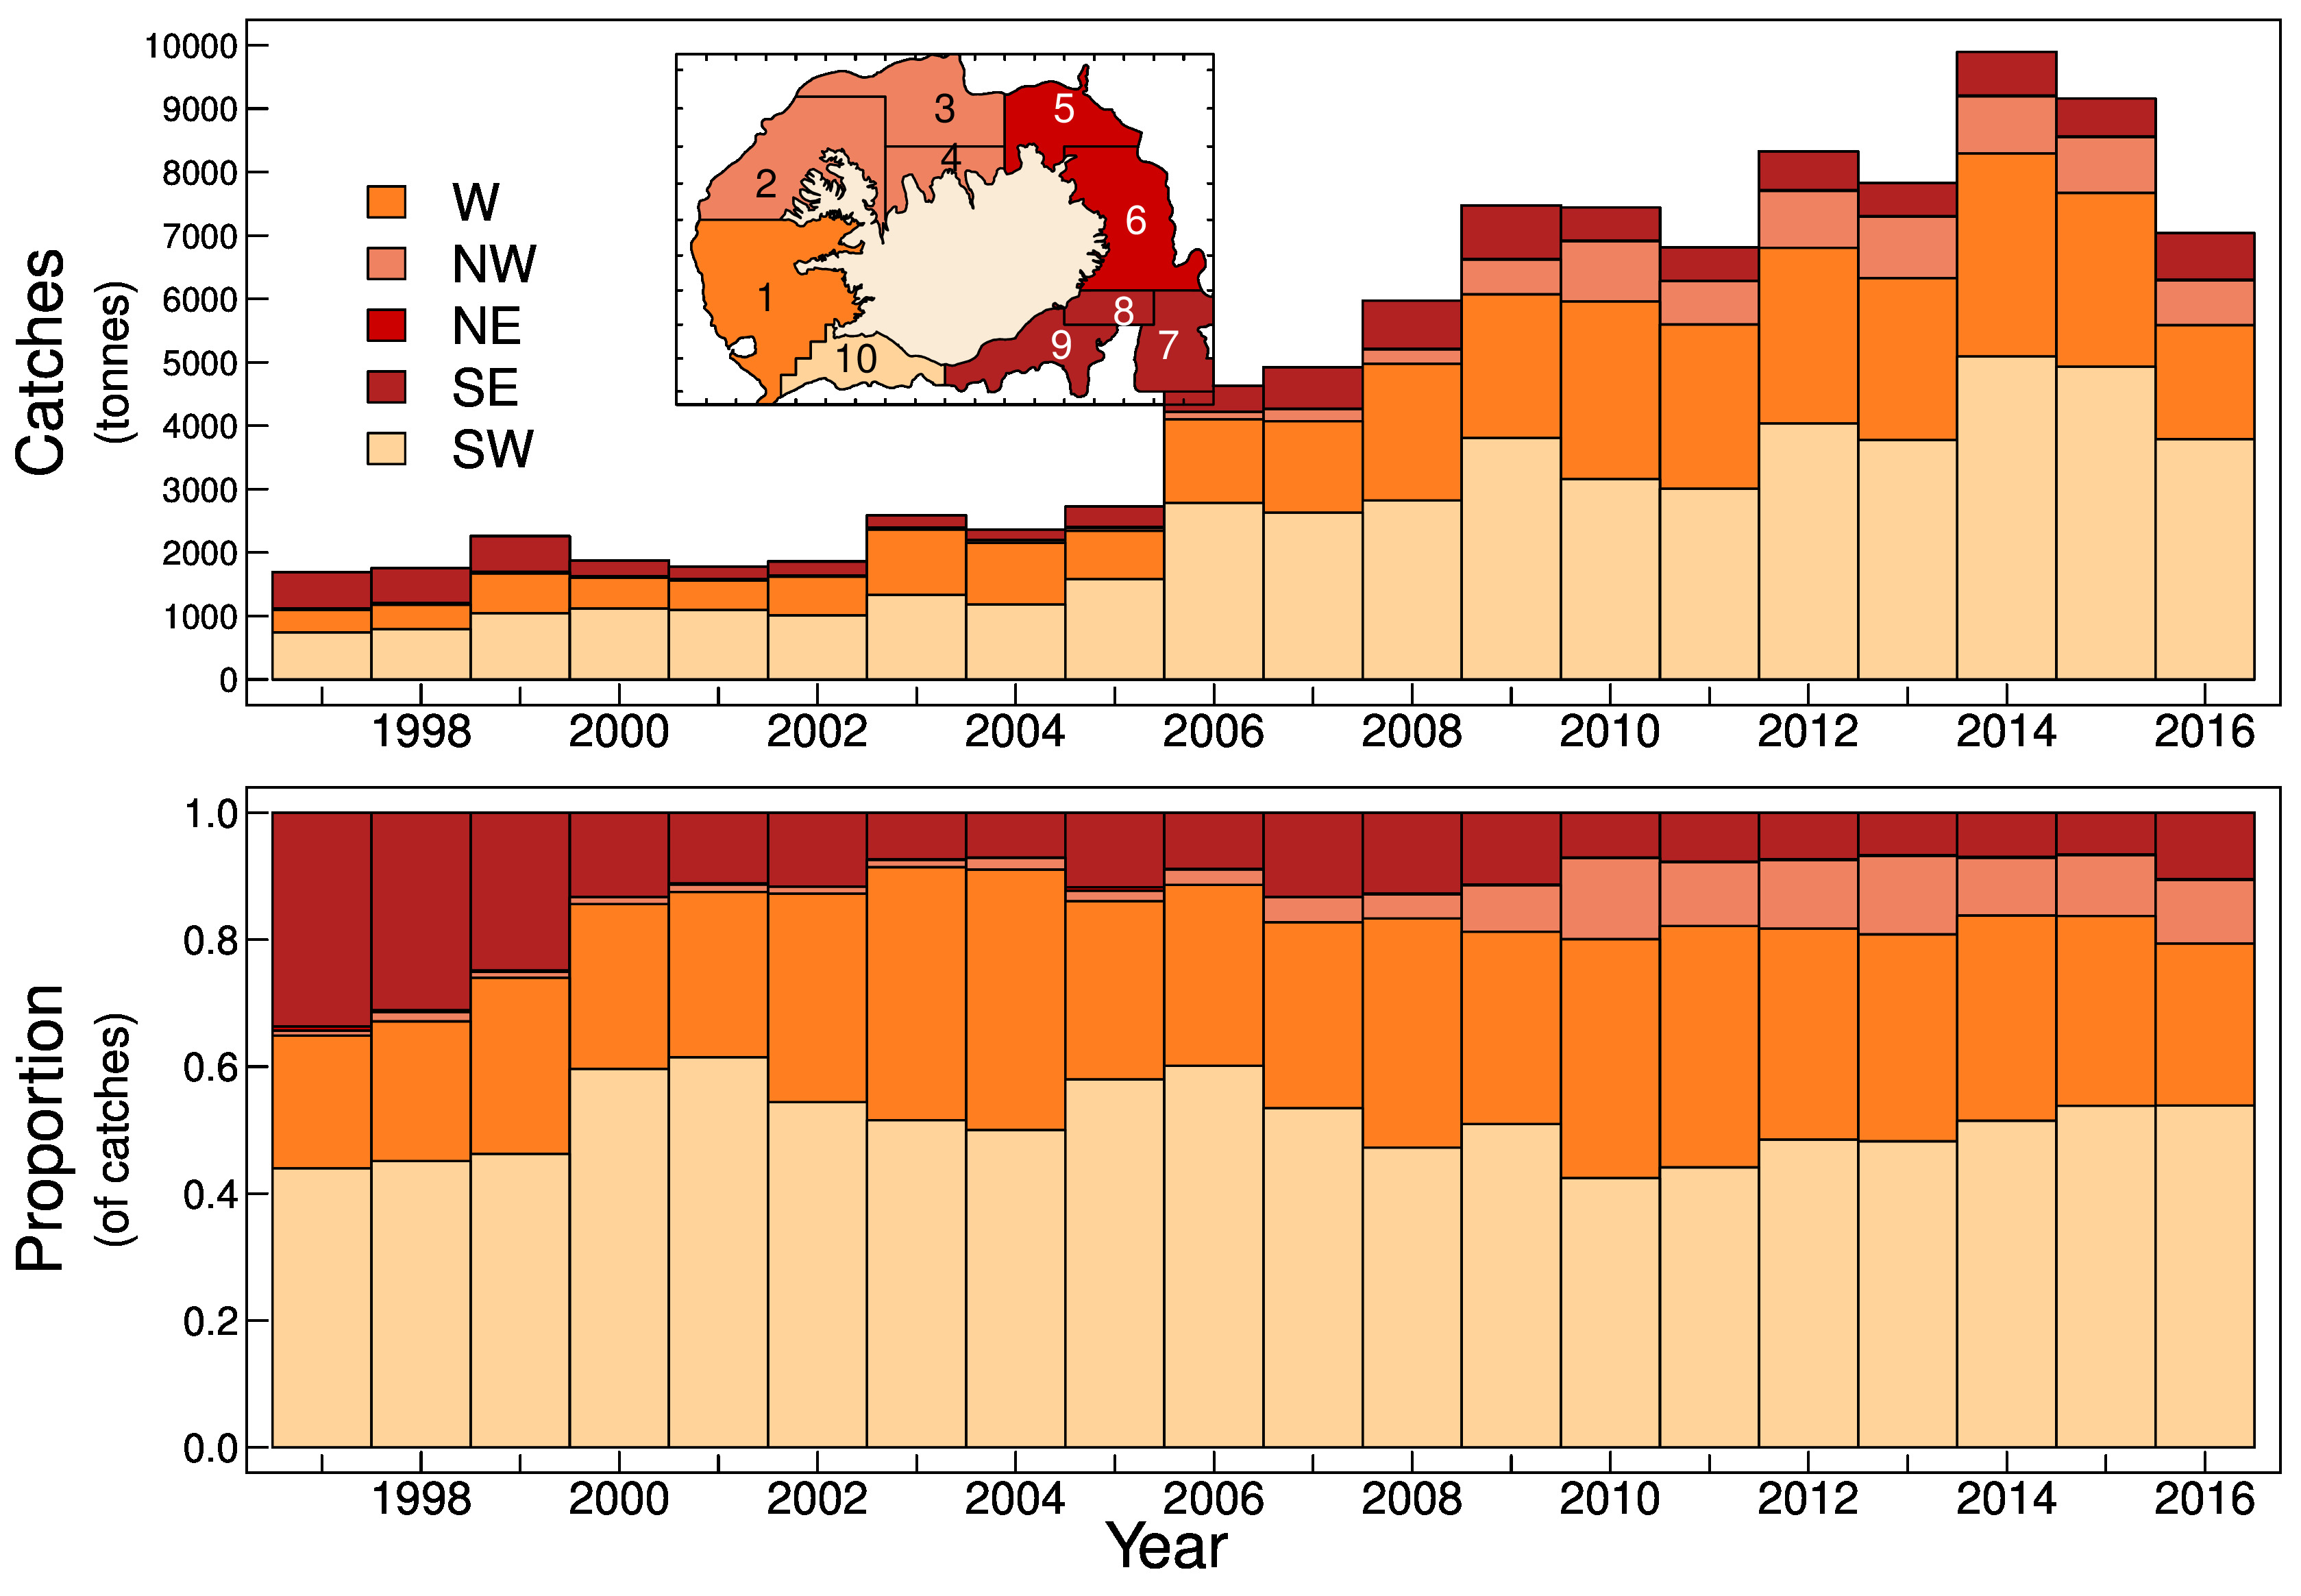
\includegraphics[width=0.7\linewidth, angle=0]{SpatialDist.jpg}
% \par}
% \end{frame}
% \frame{
% \frametitle{Initial population}
% <<echo=FALSE,results='asis',fig.width=10, fig.height=5,cache=TRUE,warning=FALSE,message=FALSE>>=
% fit$stock.std%>%
%   filter(year == 1982) %>%
%   #group_by(model,age) %>%
%   group_by(age) %>%
%   summarise(number=sum(number)) %>%
%   ggplot(aes(age,number/1e6,group=round(age))) + geom_boxplot() +
%   geom_line(data=fit$stock.std %>%
%               filter(year == 1982)%>%
%               group_by(age) %>%
%               summarise(number=sum(number)),aes(group=1),col='red') +
%   labs(y='Initial age structure (in millions)',x='Year') +
%   theme_light()
% @
% 
% }

% \frame{
% \frametitle{Equilibrium yield and SSB}
% <<yield,echo=FALSE,results='asis',fig.width=10, fig.height=5,cache=TRUE,warning=FALSE,message=FALSE>>=
%  bpa <-
%   fit$res.by.year %>%
%   filter(grepl('mat',stock)) %>%
%   ungroup() %>%
%   filter(total.biomass==min(total.biomass)) %>%
%   transmute(total.biomass=total.biomass/1e6) %>%
%   unlist()
% 
% blim <- bpa/1.4
% 
% Hmsy <-
%   res2 %>%
%   filter(mlnd==max(mlnd)) %>%
%   select(rate,mF)
% 
% Hlim <-
%   res20 %>%
%   filter(mssb < blim) %>%
%   head(1) %>%
%   bind_rows(  res20 %>%
%                 filter(mssb >= blim) %>%
%                 tail(1)) %>%
%   dplyr::mutate(rate=as.numeric(rate)) %>%
%   dplyr::summarise(rate = rate[2]*(blim-mssb[1])/abs(mssb[1]-mssb[2]) + rate[1]*(mssb[2]-blim)/abs(mssb[1]-mssb[2]),
%             mF = mF[2]*(blim-mssb[1])/abs(mssb[1]-mssb[2]) + mF[1]*(mssb[2]-blim)/abs(mssb[1]-mssb[2]))
% 
% upper <- Hlim$mF/exp(1.645*0.25)
% Hpa <-
%   res20 %>%
%   filter(mF < upper & mF > Hmsy$mF & rate < 0.5) %>%
%   tail(1) %>%
%   bind_rows(  res20 %>%
%                 filter(mF >= upper & rate < 0.5) %>%
%                 head(1)) %>%
%   dplyr::mutate(rate=as.numeric(rate)) %>%
%   dplyr::summarise(rate = rate[2]*(upper-mF[1])/abs(mF[1]-mF[2]) + rate[1]*(mF[2]-upper)/abs(mF[1]-mF[2]),
%             mF = upper)
% 
% 
% yield.plot <-
%   res20 %>%
%   bind_rows(res2,.id='meth') %>%
%   #filter(!(rate %in%c(0.46,0.52))) %>%
%   ggplot(aes(as.numeric(rate),mlnd,group=1)) +
%   geom_ribbon(aes(ymin=llnd,ymax=ulnd),fill='gold') +
%   geom_ribbon(aes(ymin=mlndq5,ymax=mlndq95),fill='gold',alpha=0.5) +
%   geom_line() +
%   #xlim(c(0.01,1)) +
%   geom_vline(xintercept = Hmsy$rate %>% as.numeric())+
%   geom_vline(xintercept = Hpa$rate, lty=2) +
%   geom_vline(xintercept = Hlim$rate, col='red')+
%   theme_light() +
%   labs(x='Harvest rate (H)', y='',title='Avg. yield (in kt)') +
%   scale_x_continuous(breaks = seq(0,0.5,by=0.1)) +
%   xlim(c(0,0.7)) +
%   facet_wrap(~meth,ncol=1) +
%   theme(strip.background = element_blank(),strip.text=element_blank())
% ssbmsy <-
%   res20 %>%
%   bind_rows(res2,.id='meth') %>%
%   #filter(!(rate %in%c(0.46,0.52))) %>%
%   ggplot(aes(as.numeric(rate),mssb,group=1)) +
%   geom_rect(ymin=-Inf,ymax=blim,xmin=-Inf,xmax=Inf,fill='red',alpha=0.1) +
%   geom_ribbon(aes(ymin=lssb,ymax=ussb),fill='gold') +
%   geom_ribbon(aes(ymin=mssbq5,ymax=mssbq95),fill='gold',alpha=0.5) +
%   geom_line() +
%   #ylim(c(0,)) +
%   geom_vline(xintercept = Hmsy$rate %>% as.numeric())+
%   geom_vline(xintercept = Hpa$rate, lty=2) +
%   geom_vline(xintercept = Hlim$rate, col='red')+
%   theme_light() +
%   labs(x='Harvest rate (H)', y='',title='Avg. SSB (in kt)')+
%   scale_x_continuous(breaks = seq(0,1,by=0.1)) +
%   xlim(c(0,0.7)) +
%   facet_wrap(~meth,ncol=1)  +
%   theme(strip.background = element_blank(),strip.text=element_blank())
% 
% gridExtra::grid.arrange(yield.plot,ssbmsy,ncol=2)
% @
% }
% 
% 
% \frame{
% \frametitle{Projections}
% 
% \item will be replaced with projection plots of this years prognosis
% <<echo=FALSE,results='asis',fig.width=10, fig.height=5,cache=TRUE,warning=FALSE,message=FALSE>>=
% rates <- c(0.18,0.2,0.24)
% 
% ssb_progn.plot <-
% res_by_year %>%
% #  bind_rows(.id='rate') %>%
%   filter(rate %in% rates,year < 2050) %>%
%   select(c(year,rate,matches("ssb"))) %>%
%   ggplot(aes(year,mssb/1e6)) +
%   geom_ribbon(aes(ymin=lssb/1e6,ymax=ussb/1e6),fill='gold',alpha=0.5) +
%   geom_ribbon(aes(ymin=llssb/1e6,ymax=uussb/1e6),fill='gold',alpha=0.5) +
%   geom_line() +
%   geom_line(aes(y=ssb6/1e6),lty=2) +
%   geom_line(aes(y=ssb542/1e6),lty=3) +
%   geom_line(aes(y=ssb931/1e6),lty=4) +
%   geom_vline(xintercept = lastyear,lty=2) +
%   facet_wrap(~rate,ncol=1) +
%   theme_light() +
%   labs(title='SSB (in kt)',x='Year',y='') +
%   geom_hline(yintercept = bpa,lty=2) +
%   geom_hline(yintercept = blim,col='red')+
%   expand_limits(y=0)
% 
% catch_progn.plot <-
% res_by_year %>%
% #  bind_rows(.id='rate') %>%
%   filter(year>lastyear,rate %in% rates,year < 2050) %>%
%   select(c(year,rate,matches("lnd"))) %>%
%   bind_rows(fit$res.by.year %>%
%               group_by(year) %>%
%               dplyr::summarise(mlnd=sum(catch/4)) %>%
%               left_join(expand.grid(year=1982:lastyear,
%                                     rate=as.character(rates))))%>%
%   ggplot(aes(year,4*mlnd/1e6)) +
%   geom_ribbon(aes(ymin=4*llnd/1e6,ymax=4*ulnd/1e6),fill='gold',alpha=0.5) +
%   geom_ribbon(aes(ymin=4*lllnd/1e6,ymax=4*uulnd/1e6),fill='gold',alpha=0.5) +
%   geom_line() +
%   geom_line(aes(y=lnd6/1e6),lty=2) +
%   geom_line(aes(y=lnd542/1e6),lty=3) +
%   geom_line(aes(y=lnd931/1e6),lty=4) +
%   geom_vline(xintercept = lastyear,lty=2) +
%   facet_wrap(~rate,ncol=1) +
%   theme_light() +
%   labs(title='Catches (in kt)',x='Year',y='') +
%   expand_limits(y=0)
% 
% f_progn.plot <-
%   res_by_year %>%
%   filter(year>(lastyear+1)) %>%
%   bind_rows(fit$res.by.year %>%
%               filter(grepl('mat',stock)) %>%
%               group_by(year) %>%
%               dplyr::summarise(mF=mean(F),
%                         uuF=quantile(F,0.75),
%                         llF=quantile(F,0.25),
%                         uF = quantile(F,0.95),
%                         lF = quantile(F,0,05)) %>%
%               left_join(expand.grid(year=1982:lastyear,
%                                     rate=as.character(rates))))%>%
% #  bind_rows(.id='rate') %>%
%   filter(rate %in% rates,year < 2050) %>%
%   #select(c(year,rate,)) %>%
%   ggplot(aes(year,mF)) +
%   geom_ribbon(aes(ymin=lF,ymax=uF),fill='gold',alpha=0.5) +
%   geom_ribbon(aes(ymin=llF,ymax=uuF),fill='gold',alpha=0.5) +
%   geom_line() +
%   geom_line(aes(y=F6),lty=2) +
%   geom_line(aes(y=F542),lty=3) +
%   geom_line(aes(y=F931),lty=4) +
%   geom_vline(xintercept = (lastyear+1),lty=2) +
%   geom_hline(yintercept = Hlim$mF,col='red')+
%   geom_hline(yintercept = Hpa$mF,lty=2)+
%   facet_wrap(~rate,ncol=1) +
%   theme_light() +
%   labs(title='Fishing mortality',x='Year',y='') +
%   expand_limits(y=0)
% 
% rec_progn.plot <-
% res_by_year %>%
%   filter(rate %in% rates,year < 2050) %>%
%   select(rate,year,matches('rec')) %>%
%   ggplot(aes(year,mrec/1e6)) +
%   geom_ribbon(aes(ymin=lrec/1e6,ymax=urec/1e6),fill='gold',alpha=0.5) +
%   geom_ribbon(aes(ymin=llrec/1e6,ymax=uurec/1e6),fill='gold',alpha=0.5) +
%   geom_line() +
%   geom_line(aes(y=rec6/1e6),lty=2) +
%   geom_line(aes(y=rec542/1e6),lty=3) +
%   geom_line(aes(y=rec931/1e6),lty=4) +
%   geom_vline(xintercept = (lastyear+1),lty=2) +
%   facet_wrap(~rate,ncol=1) +
%   theme_light() +
%   labs(title='Recruitment (in millions)',x='Year',y='') +
%   expand_limits(y=0)
% 
% gridExtra::grid.arrange(catch_progn.plot,ssb_progn.plot,f_progn.plot,rec_progn.plot,ncol=4)
% @
% }


% 
% \frame{
% \frametitle{Objective function}
% \bi The total objective function used the modeling process combines the contribution of each data set using the following formula:
% 
% 
% \begin{equation}\label{eq:loglik}
% l^{\textup{T}} = \sum_g  w_{gf}^{\textup{SI}}
% l_{g,S}^{\textup{SI}} + \sum_{f\in \{S,C\}} \left(
%   w_{f}^{\textup{LD}}  l_{f}^{\textup{LD}} + w_{f}^{\textup{AL}}
%   l_{f}^{\textup{AL}}\right) + w^{\textup{M}}l^{\textup{M}}
% \end{equation}
% where $f=S$, $L$, $G$, $B$ denotes the spring survey, and the commercial fleets respectively
% and $w$'s are the weights assigned to each likelihood component.
% \item For each length range $g$ the survey index is compared to the modeled
% abundance at year $y$ and time-step $t$ using:
% \begin{equation}\label{eq:SSSI}
%   l_{g}^{\textup{SI}} = \sum_{y} \sum_t (\log I_{gy} - (\log q_g + b_g \log \widehat{N_{gyt}}))^2
% \end{equation}
% where $$\widehat{N_{gyt}} = \sum_{l\in g} \sum_a \sum_s N_{alsyt}$$
% \item For compositional data the likelihood is of the form:
% \begin{equation}\label{eq:SSldist}
%   l_f^{\textup{LD}} = \sum_y \sum_t \sum_l (\pi_{flyt} - \hat{\pi}_{flyt})^2
% \end{equation}
% \ei
% 
% }
% 
% \frame{
% \frametitle{Weighting heuristic}
% \begin{enumerate}
% \item Calculate the initial sums of squares (SS) given the initial
%   parametrization for all likelihood components. Assign the inverse SS
%   as the initial weight for all likelihood components.
% \item For each likelihood component, do an optimization run with
%   the initial SS for that component set to 10000. Then estimate the
%   residual variance using the resulting SS of that component divided
%   by the degrees of freedom ($df^*$), i.e. $\hat{\sigma}^2 = \frac{SS}{df^*}$.
% \item  After the optimization set the final weight for that all
%   components as the inverse of the estimated variance from the step above
%   (weight $=1/\hat{\sigma}^2$).
% \end{enumerate}
% 
% }
% 
% 
% 
% \frame{
% \frametitle{Uncertainty estimates}
% <<divisionplot2,echo=FALSE,results='asis',fig.width=10, fig.height=5,cache=TRUE,warning=FALSE,message=FALSE>>=
% 
% 
% reitmapping <-
%   read.table(
%         system.file("demo-data", "reitmapping.tsv", package="mfdb"),
%         header=TRUE,
%         as.is=TRUE) %>%
%   dplyr::mutate(sr=as.numeric(GRIDCELL)) %>%
%   mar:::sr2d() %>%
%   filter(SUBDIVISION %in% tmp$division)
% 
% 
% 
% test <-
%   plyr::ddply(reitmapping, 'SUBDIVISION',
%         function(x){
%           ##   2
%           ## 1 x 3
%           ##   4
%           sides <- rep(10*x$GRIDCELL,each=4) + 1:4
%           up <- geo::d2sr(x$lat + 0.125, x$lon)
%           down <- geo::d2sr(x$lat - 0.126, x$lon)
%           left <- geo::d2sr(x$lat, x$lon - 0.25)
%           right <- geo::d2sr(x$lat, x$lon + 0.26)
% 
%           for(i in 1:nrow(x)){
%             ## up
%             if(up[i] %in% x$GRIDCELL){
%               sides[4*(i-1)+2] <- NA
%               sides[sides==(10*up[i]+4)] <- NA
%             }
%             ## down
%             if(down[i] %in% x$GRIDCELL){
%               sides[4*(i-1)+4] <- NA
%               sides[sides==(10*down[i]+2)] <- NA
%             }
%             ## left
%             if(left[i] %in% x$GRIDCELL){
%               sides[4*(i-1)+1] <- NA
%               sides[sides==(10*left[i]+3)] <- NA
%             }
%             ## right
%             if(right[i] %in% x$GRIDCELL){
%               sides[4*(i-1)+3] <- NA
%               sides[sides==(10*right[i]+1)] <- NA
%             }
%           }
%           sides <- sides[!is.na(sides)]
%           corners <- plyr::ddply(data.frame(side=rep(sides,each=2)),
%                        'side',
%                        function(x){
%                          loc <- geo::sr2d(floor(x$side[1]/10))
%                          loc <- c(loc$lat,loc$lon)
%                          if((x$side[1] %% 10) == 1){
%                            up.loc <- loc+c(0.125,-0.25)
%                            down.loc <- loc+c(-0.125,-0.25)
%                          }
%                          if((x$side[1] %% 10) == 3){
%                            up.loc <- loc+c(0.125,0.25)
%                            down.loc <- loc+c(-0.125,0.25)
%                          }
%                          if((x$side[1] %% 10) == 2){
%                            up.loc <- loc+c(0.125,-0.25)
%                            down.loc <- loc+c(0.125,0.25)
%                          }
%                          if((x$side[1] %% 10) == 4){
%                            up.loc <- loc+c(-0.125,-0.25)
%                            down.loc <- loc+c(-0.125,0.25)
%                          }
%                          tmp <- as.data.frame(rbind(up.loc,down.loc))
%                          names(tmp) <- c('lat','lon')
%                          return(tmp)
%                        })
%           corners$order <- NA
%           corners$order[1:2] <- 1:2
%           counter <- 1:nrow(corners)
%           i <- 2
%           for(order in 3:(length(sides))){
%             tmp <- counter[is.na(corners$order) &
%                            corners$lat == corners$lat[i] &
%                            corners$lon == corners$lon[i]][1]
%             corners$order[corners$side == corners$side[tmp]] <- order
%             corners <- corners[-tmp,]
%             i <- which(corners$order == order)
% 
%           }
%           corners$side <- NULL
%           return(arrange(corners,order))
% 
%         })
% 
% bcareas <- c(1015, 1014, 1018, 1011, 1012, 1023, 1023, 1021, 1032, 1031,
%              1042, 1041, 1052, 1053, 1051, 1054, 1061, 1071, 1081, 1082)
% 
% 
%  ggplot(data.frame(lat=0,lon=0), aes(lon,lat)) +
% #  ggplot(subset(dat,ar==2011),aes(lon,lat)) +
% #  stat_density2d(aes(fill=..level..),geom='polygon') +
% #  scale_fill_gradient(limits = c(0,0.2), low='yellow',high='red') +
%   geom_point(col='yellow') +
%   geom_path(data=geo::gbdypi.100,lty=2,size = 0.3) +
%   geom_path(data=geo::gbdypi.800,lty=2,size = 0.3) +
%   #  geom_polygon(alpha=0.5,data=geo::gbdypi.100,fill='gray90') +
%   geom_path(data=geo::gbdypi.200,lty=2,size = 0.3) + #alpha=0.5,fill='gray90',
%   geom_path(data=geo::gbdypi.500,lty=3,size = 0.3) +
%   geom_path(data=geo::gbdypi.1000,lty=4,size = 0.3) +
%   geom_path(aes(lon,lat,group=SUBDIVISION),
%             data=test, #
%             #subset(test,SUBDIVISION %in% bcareas),
%             size = 0.3) +
%  # geom_polygon(aes(lon,lat,group=SUBDIVISION),
%   #          data=test %>%
%    #           filter(SUBDIVISION %in% c(1061,1143,1142)), #
%     #        #subset(test,SUBDIVISION %in% bcareas),
%      #       size = 0.3,fill='gold',alpha=0.5) +
% 
%   geom_polygon(data=geo::island, col = 'black' ,fill = 'gray70',size = 0.3) +
% #  geom_polygon(data=geo::greenland, col = 'black', fill = 'gray70') +
%   geom_polygon(data=geo::eyjar, col = 'black', fill = 'gray70',size = 0.3) +
%   geom_polygon(data=geo::faeroes, col = 'black', fill = 'gray70') +
%   coord_map('mercator', xlim=c(-30,-10),ylim=c(62,68)) +
% #     geom_label(aes(lon,lat,label=SUBDIVISION),
% #            data=ddply(test,~SUBDIVISION, summarise, lat=mean(lat),
% #              lon=mean(lon))) +
% #  coord_map('mercator', xlim=c(-28,-9.5),ylim=c(62.5,68)) +
%   xlab('Longitude') +
%   ylab('Latitude') +
%   theme_light() +
%   #geom_point(data=tmp %>% select(tow,lat,lon) %>% distinct()) +
%   geom_path(data = geo::twohmiles, lty = 2) #+
% #  geom_path(data=icelandrivers,size=0.1,col='blue') +
% #  geom_path(data=glaciers,size=0.5)
% @
% }
% 
% \frame{
% \frametitle{Order of calculations}
% The order of calculations is as follows:
% \begin{enumerate}
% \item \textbf{Printing}: model output at the beginning of the time-step
% \item \textbf{Consumption}: mainly fleet harvesting
% \item \textbf{Natural mortality}: Natural mortality is applied after consumption
% \item \textbf{Growth}: length update is applied
% \item \textbf{Maturation}: maturing fish moved from one stock component to the other
% \item \textbf{Spawning and recruitment}: New individuals enter the immature stock component
% \item \textbf{Likelihood comparison}: likelihood score is calculated here, note that the comparison is based on the modeled processes in previous steps
% \item \textbf{Printing}: model output at the end of the time-step
% \item \textbf{Aging}: if this is the end of year the age is increased
% \end{enumerate}
% }
% 
% 
% \frame{
% \frametitle{Likelihood values - compositional data}
% <<echo=FALSE,results='asis',fig.width=10, fig.height=5,cache=TRUE,warning=FALSE,message=FALSE>>=
% 
% fit$likelihoodsummary %>%
%   filter(component!='understocking') %>%
%   #filter(!(model %in% c(22,70,73,24,56,64)))%>%
%   left_join(SS$weights, by=c("component"="Component"),copy=TRUE) %>%
%   filter(!grepl('si\\.',component)) %>%
%   mutate(year = as.numeric(year),
%          step = as.numeric(step),
%          t = year + (step-1)/4,
%          score = likelihood.value*Weight) %>%
%   ggplot(aes(t,score,group=interaction(round(year)))) + geom_boxplot() +
%   facet_wrap(~component,ncol=3) + theme_light() + ylim(c(0,750))+
%   labs(x='Year',y='Weighted scored') +
%    geom_label(data=fit$likelihoodsummary %>%
%                 filter(!grepl('si\\.',component)) %>%
%                 select(component) %>%
%                 distinct(),
%               aes(label=component,group=1),x=-Inf,y=Inf,size=3, vjust = 1.1,hjust=-0.1) +
%    theme(strip.background = element_blank(),strip.text=element_blank())
% @
% 
% }
% 
% \frame{
% \frametitle{Likelihood values - survey indices}
% 
% <<echo=FALSE,results='asis',fig.width=10, fig.height=5,cache=TRUE,warning=FALSE,message=FALSE>>=
% fit$likelihoodsummary %>%
%   left_join(SS$weights, by=c("component"="Component"),copy=TRUE) %>%
%   filter(grepl('si\\.',component)) %>%
%   dplyr::mutate(score = likelihood.value*Weight) %>%
%   ggplot(aes(component,score))+ geom_boxplot() + theme_light() +
%   labs(x='Component',y='Weighted scored')
% @
% 
% 
% }
% 
% 
% 

% \frame{
% \frametitle{Analytical retrospective}
%  <<echo=FALSE,results='asis',fig.width=10, fig.height=5,warning=FALSE,message=FALSE>>=
%  retro.res <-
%    retro.fit$res.by.year %>%
%    bind_rows(fit$res.by.year %>% dplyr::mutate(model="0")) %>%
%    group_by(year,model) %>%
%    dplyr::summarise(tb=sum(total.biomass),
%              ssb=sum(total.biomass[grepl('mat',stock)]),
%              F = max(F),
%              catch = sum(catch),
%              #hb=sum(harv.biomass),
%              rec=sum(recruitment,na.rm=TRUE)) %>%
%    left_join(retro.fit$stock.full %>%
%                filter(length>ref.cm) %>%
%                group_by(year,model) %>%
%                dplyr::summarise(hb=sum(number*mean.weight))) %>%
%    mutate(hr = catch/hb)
% 
% 
% 
%  rbio.plot <-
%    bio.plot +
%    geom_line(data= retro.res %>%
%                select(year,tb,hb,model) %>%
%                gather(col,value,-c(year,model)) %>%
%                dplyr::mutate(value=value/1e6),
%              aes(year,value,lty=model,group=interaction(model,col)),col='red') +
%    guides(linetype=FALSE)
% 
%  rssb.plot <-
%    ssb.plot +
%    geom_line(data= retro.res %>%
%                select(year,value=ssb,model) %>%
%                #gather(col,value,-c(year,model)) %>%
%                dplyr::mutate(value=value/1e6),
%              aes(year,value,lty=model,group=model),col='red')
% 
%    #ggplot(aes(year,value,lty=model,col=col)) + geom_line() +
%    #theme_light() +
%  #  labs(y='Biomass (in kt)',x='Year')+
%  #  theme(legend.position = 'none')+ expand_limits(y=0)
% 
%  rF.plot <-
%   F.plot +
%    geom_line(data=retro.res %>%
%                select(year,value=F,m=model),
%              aes(y=value,lty=m,group=m),col='red') +
%      geom_line(data=retro.res %>%
%                select(year,value=hr,m=model),
%              aes(y=value,lty=m,group=m),col='red') +
%    theme(legend.position = 'none')
%    #gather(col,value,-c(year,model)) %>%
%    #mutate(value=value/1e6) %>%
%    #ggplot(aes(year,value,lty=model)) + geom_line() +
%    #theme_light() +
%    #labs(y='Fishing mortality',x='Year')+
%    #theme(legend.position = 'none')+ expand_limits(y=0)
% 
% 
%  rrec.plot <-
%    rec.plot +
%    geom_line(data = retro.res %>%
%                select(year,value=rec,model) %>%
%                dplyr::mutate(value=value/1e6),
%              aes(year,value,lty=model,group=model),col='red')+
%    theme(legend.position = 'none')
% 
%  gridExtra::grid.arrange(rbio.plot,rssb.plot, rF.plot,rrec.plot,ncol=2)
%  @
% }


% \frame{
% \frametitle{Fit to survey indices}
% <<echo=FALSE,results='asis',fig.width=10, fig.height=5,cache=TRUE,warning=FALSE,message=FALSE>>=
% fit$sidat %>%
%   ggplot(aes(log(predict),log(number.x))) +
%   geom_line(aes(log(number.x),log(number.x)),lty=2) +
%   geom_line(aes(log(predict),log(predict)),lty=2) +
%   facet_wrap(~name, scale='free') +
%   geom_text(aes(label=year),size=3) +
%   #scale_x_log10() +
%   #scale_y_log10() +
%   theme_light() +
%   labs(y='log(Observed)',x='log(Predicted)')+
%   geom_label(data=fit$sidat %>%
%               select(name,slope,sse) %>%
%               distinct() %>%
%               dplyr::mutate(label=paste(name,paste0('sse:',sse),sep='\n')),
%             aes(label=label),x=Inf,y=-Inf,size=3, vjust = -0.1,hjust=1.1) +
%   theme(strip.background = element_blank(),strip.text=element_blank())
% 
% @
% }


% \frame{
% \frametitle{Parameter correlations}
% <<echo=FALSE,results='asis',fig.width=10, fig.height=5,cache=TRUE,warning=FALSE,message=FALSE>>=
% fit$params %>%
%   filter(optimise==1,
%          !grepl('rec\\.[0-9]',switch),
%          !grepl('init\\.[0-9]',switch),
%          !grepl('scalar',switch)) %>%
%   mutate(switch = gsub('^[A-Za-z]+\\.','',switch),
%          value = ifelse(grepl('k$|mat1$',switch),0.001*value,value),
%          label = forcats::fct_recode(switch,
%                                      'beta' = "bbin",
%                                      'alpha[c]' = 'comm.alpha',
%                                      'l[50][c]' ='comm.l50',
%                                      'alpha[s]' = 'igfs.alpha',
%                                      'l[50][s]'='igfs.l50',
%                                      'F[0]'='init.F',
%                                      'L[infinity]'='Linf',
%                                      'lambda'='mat1',
%                                      'l[50]'='mat2',
%                                      'sigma[0]'='rec.sd',
%                                      'l[0]'='recl' )) %>%
%   select(model,switch,value) %>% spread(switch,value) %>% select(-model) %>%
%   GGally::ggpairs() +
%   theme_light()
% @
% 
% }


% \frame{
% \frametitle{Parameter estimates}
% <<echo=FALSE,results='asis',fig.width=10, fig.height=5,cache=TRUE,warning=FALSE,message=FALSE>>=
% fit$params %>%
%   #filter(!(model %in% c(22,70,73,24,56,64)))%>%
%   filter(optimise==1,
%          !grepl('rec\\.[0-9]',switch),
%          !grepl('init\\.[0-9]',switch),
%          !grepl('scalar',switch)) %>%
%   mutate(switch = gsub('^[A-Za-z]+\\.','',switch),
%          value = ifelse(grepl('k$|mat1$',switch),0.001*value,value),
%          label = forcats::fct_recode(switch,
%                                      'beta' = "bbin",
%                                      'alpha[g]' = 'gil.alpha',
%                                       'l[50][g]' ='gil.l50',
%                                      'alpha[l]' = 'lln.alpha',
%                                       'l[50][l]' ='lln.l50',
%                                      'alpha[t]' = 'bmt.alpha',
%                                       'l[50][t]' ='bmt.l50',
%                                      'alpha[s]' = 'igfs.alpha',
%                                       'l[50][s]'='igfs.l50',
%                                      'F[0]'='init.F',
%                                      'L[infinity]'='Linf',
%                                      'lambda'='mat1',
%                                      'l[50]'='mat2',
%                                      'sigma[0]'='rec.sd',
%                                       'l[0]'='recl'  )) %>%
%   ggplot(aes(value)) + geom_histogram(fill='gray')+
%   facet_wrap(~label,scale='free',labeller = label_parsed) +
%   geom_vline(aes(xintercept=value),
%              col='red',
%              data=fit$params %>%
%                filter(optimise==1,
%                       !grepl('rec\\.[0-9]',switch),
%                       !grepl('init\\.[0-9]',switch),
%                       !grepl('scalar',switch)) %>%
%               mutate(switch = gsub('^[A-Za-z]+\\.','',switch),
%                      value = ifelse(grepl('k$|mat1$',switch),0.001*value,value),
%                      label = forcats::fct_recode(switch,
%                                      'beta' = "bbin",
%                                      'alpha[g]' = 'gil.alpha',
%                                       'l[50][g]' ='gil.l50',
%                                      'alpha[l]' = 'lln.alpha',
%                                       'l[50][l]' ='lln.l50',
%                                      'alpha[t]' = 'bmt.alpha',
%                                       'l[50][t]' ='bmt.l50',
%                                      'alpha[s]' = 'igfs.alpha',
%                                       'l[50][s]'='igfs.l50',
%                                      'F[0]'='init.F',
%                                      'L[infinity]'='Linf',
%                                      'lambda'='mat1',
%                                      'l[50]'='mat2',
%                                      'sigma[0]'='rec.sd',
%                                       'l[0]'='recl' ))) +
%   theme_light() +
%   labs(x='Parameter value',y='% iterations')
% 
% @
% }
%
% \frame{
% \frametitle{Survey indices}
% \begin{columns}
% \begin{column}{0.5\linewidth}
% <<echo=FALSE,results='asis'>>=
% fit$sidat %>%
%   filter(!is.na(number.x)) %>%
%   group_by(name,length) %>%
%   dplyr::summarise(n=sum(number.x),range=paste(lower,upper,sep=' -- ')[1],or=lower[1]) %>%
%   arrange(or) %>%
%   select(name,range,n) %>%
%   knitr::kable()
% @
% \end{column}
% \begin{column}{0.5\linewidth}
% <<echo=FALSE,cache=TRUE>>=
% fit$catchdist.fleets %>%
%   filter(name=='ldist.igfs',year %in% 2010:2013) %>%
%   ggplot(aes(lower,number.x))+
%   geom_rect(fill='darkblue',alpha=0.01,xmin=20,xmax=52,ymin=-Inf,ymax=Inf)+
%   geom_rect(fill='darkblue',alpha=0.01,xmin=60,xmax=72,ymin=-Inf,ymax=Inf)+
%   geom_rect(fill='darkblue',alpha=0.01,xmin=80,xmax=92,ymin=-Inf,ymax=Inf)+
%   geom_rect(fill='darkblue',alpha=0.01,xmin=100,xmax=160,ymin=-Inf,ymax=Inf)+
%   geom_line() + facet_wrap(~year,scale='free_y') +
%   theme_minimal() + labs(x='Length', y='Number observed')
% @
% \end{column}
% \end{columns}
% }
%
% \frame{
% \frametitle{Available samples from the Icelandic groundfish survey}
% <<echo=FALSE,results='asis',fig.width=10, fig.height=5>>=
% fit$catchdist.fleets %>%
%   filter(name %in% c('aldist.igfs','ldist.igfs')) %>%
%   group_by(name,year) %>%
%   dplyr::summarise(n=sum(number.x,na.rm=TRUE)) %>%
%   bind_rows(fit$stockdist %>%
%               as.data.frame() %>%
%               select(year,name,number.x) %>%
%               group_by(year,name) %>%
%               dplyr::summarise(n=sum(number.x,na.rm=TRUE))) %>%
%   ggplot(aes(year,n)) + geom_bar(stat = 'identity',fill='#0076a9') + facet_wrap(~name,ncol=1,scale='free_y') +
%   theme_minimal() +
%   labs(y='Num. samples',x='Year')
% @
%
% }
%
%
% \frame{
% \frametitle{Available samples from commercial catches}
% <<echo=FALSE,results='asis',fig.width=10, fig.height=5,cache=TRUE>>=
% fit$catchdist.fleets %>%
%   filter(!(name %in% c('aldist.igfs','ldist.igfs','matp.igfs'))) %>%
%   group_by(name,year) %>%
%   dplyr::summarise(n=sum(number.x,na.rm=TRUE)) %>%
%   mutate(type = ifelse(grepl('aldist',name),'Age - Length','Length'),
%          gear = gsub('[a-z]+\\.','',name))%>%
%   ggplot(aes(year,n,fill=gear)) + geom_bar(stat = 'identity') + facet_wrap(~type,ncol=1,scale='free_y') +
%   theme_minimal() +
%   labs(y='Num. samples',x='Year') +
%   theme(legend.position = c(0.1,0.8))
% @
%
% }
%
% \frame{
% \frametitle{Landings data}
%
% \begin{columns}
% \begin{column}{0.5\linewidth}
% Sources of landings data:
% \bi Landings of Icelandic vessels:
%   \bi Pre 1993: landings by port from Fiskifélagið
%   \item Post 1993: Directorate of fisheries, catches reported by vessel
%   \ei
% \item Landings of foreign vessels:
%   \bi Pre 2014: Statlant
%   \item Post 2014: Directorate of fisheries, catches reported by vessel
%   \ei
% \ei
% \end{column}
% \begin{column}{0.5\linewidth}
% <<echo=FALSE,cache=TRUE>>=
% fit$fleet.info %>%
%   filter(fleet !='igfs') %>%
%   ggplot(aes(year,amount/1e6,fill=fleet)) + geom_bar(stat='identity') +
%   theme_minimal() +
%   labs(y='Landed catch (kt)',x='Year') +
%   theme(legend.position = c(0.1,0.8))
% @
% \end{column}
% \end{columns}
% }
%
% \frame{
% \frametitle{Fit to data -- Indices}
%
% <<echo=FALSE,fig.width=10, fig.height=5,cache=TRUE>>=
% fit$sidat %>%
%   mutate(group=ordered(lower,labels=paste(unique(sort(lower)),unique(sort(upper)),sep = ' - '))) %>%
%   ggplot(aes(year,number.x)) + geom_point() +
%   facet_wrap(~group,scale='free_y') +
%   geom_text(data=. %>% select(group,slope,intercept,sse) %>% distinct(), aes(label=sprintf('slope=%.2f',slope)),x=1990,y=Inf,vjust=2) +
%   theme_minimal() + geom_line(aes(y=predict)) +
%   labs(y='Survey index',x='Year')
% @
%
%
% }
%
%
% \frame{
% \frametitle{Fit to data -- survey length distributions}
% <<echo=FALSE,fig.width=10, fig.height=5,warning=FALSE,message=FALSE,cache=TRUE>>=
% fit$catchdist.fleets %>%
%   filter(name=='ldist.igfs') %>%
%   ggplot(aes(lower,observed)) + geom_point(col='gray') +
%   geom_segment(aes(xend=lower,yend=0),col='grey') +
%   facet_wrap(~year) + theme_bw() +
%   geom_line(aes(y=predicted)) + #xlim(c(25,55)) +
%   geom_label(x=50,y=0.12,aes(label=year)) +
%   geom_text(x=140,y=0.07,angle=90,aes(label=paste0('n = ',round(total.catch)))) +
%   theme(strip.background = element_blank(),strip.text=element_blank()) +
%   xlab('Length') + ylab('Proportion')
%
%
% @
%
% }
%
%
% \frame{
% \frametitle{Fit to data -- survey age distributions}
% <<echo=FALSE,fig.width=10, fig.height=5,warning=FALSE,message=FALSE,cache=TRUE>>=
% fit$catchdist.fleets %>%
%   dplyr::filter(name=='aldist.igfs') %>%
%   dplyr::mutate(age=as.numeric(gsub('age','',age)),
%                 length=as.numeric(gsub('len','',length))) %>%
%   dplyr::group_by(year,age,step,total.catch) %>%
%   dplyr::summarise(o=sum(observed,na.rm=TRUE),
%                    p=sum(predicted)) %>%
%   dplyr::mutate(o=ifelse(o==0,NA,o)) %>%
%   ggplot(aes(age,o)) + geom_point(col='gray') +
%   geom_segment(aes(xend=age,yend=0),col='grey') + facet_wrap(~year+step) +
%   theme_bw() + geom_line(aes(y=p)) +
%   geom_label(x=12,y=0.3,aes(label=year)) +
%   geom_text(x=12,y=0.15,aes(label=paste0('n = ',total.catch))) +
%   theme(strip.background = element_blank(),strip.text=element_blank()) +
%   xlab('Length') + ylab('Proportion')
% @
%
% }
%
% \frame{
% \frametitle{Fit to data -- survey growth data}
% <<echo=FALSE,fig.width=10, fig.height=5,warning=FALSE,message=FALSE,cache=TRUE>>=
% fit$catchdist.fleets %>%
%   filter(name=='aldist.igfs') %>%
%   group_by(year,step,age) %>%
%   mutate(o=observed/sum(observed,na.rm=TRUE),p=predicted/sum(predicted)) %>%
%   select(year,step,age,length,observed,o,predicted,p) %>%
%   ungroup() %>%
%   mutate(age=as.numeric(gsub('age','',age)),
%          length=as.numeric(gsub('len','',length))) %>%
%   group_by(year,step,age) %>%
%   summarise(o.ml=sum(o*length,na.rm=TRUE),
%             o.sl=sqrt(sum(o*(length - o.ml)^2,na.rm=TRUE)),
%             p.ml=sum(p*length),
%             p.sl=sqrt(sum(p*(length - p.ml)^2))) %>%
%   mutate(o.ml=ifelse(o.ml==0,NA,o.ml),
%          o.sl=ifelse(o.sl==0,NA,o.sl),
%          upper = p.ml+1.96*p.sl,
%          lower = p.ml-1.96*p.sl,
%          o.upper = o.ml+1.96*o.sl,
%          o.lower = o.ml-1.96*o.sl) %>%
%   ggplot(aes(age,o.ml)) + geom_ribbon(fill='gold',aes(ymax=upper,ymin=lower))+geom_point(size=0.5) +
%   geom_line(aes(y=p.ml))  + geom_linerange(aes(ymax=o.upper,ymin=o.lower))+
%   facet_wrap(~year+step) +
%   theme_bw() + xlab('Age') + ylab('Average length') +
%   geom_label(x=12,y=30,aes(label=year)) +
%   theme(strip.background = element_blank(),strip.text=element_blank())
% @
%
%
% }
% \frame{
% \frametitle{Fit to data -- survey maturity}
%
% <<echo=FALSE,fig.width=10, fig.height=5,warning=FALSE,message=FALSE,cache=TRUE>>=
% fit$stockdist %>%
%   filter(stock=='lingmat') %>%
%   ggplot(aes((upper+lower)/2,obs.ratio)) + geom_point() +
%   geom_line(aes(y=pred.ratio))+
%   facet_wrap(~year) + theme_minimal() +
%   labs(y='Prop. mature',x='Length')
% @
%
% }
%
% \frame{
% \frametitle{Fit to data -- lln length distributions}
% <<echo=FALSE,fig.width=10, fig.height=5,warning=FALSE,message=FALSE,cache=TRUE>>=
% fit$catchdist.fleets %>%
%   filter(name=='ldist.lln') %>%
%   ggplot(aes(lower,observed)) + geom_point(col='gray') +
%   geom_segment(aes(xend=lower,yend=0),col='grey') +
%   facet_wrap(~year+step) + theme_bw() +
%   geom_line(aes(y=predicted)) + #xlim(c(25,55)) +
%   geom_label(x=140,y=0.15, size = 2.5,
%              aes(label=sprintf('%s, q%s',year,step))) +
%   geom_text(x=140,y=0.07,angle=90,size=2.5,
%             aes(label=paste0('n = ',round(total.catch)))) +
%   theme(strip.background = element_blank(),strip.text=element_blank(),
%         axis.text.y = element_blank()) +
%   xlab('Length') + ylab('Proportion')
%
%
% @
%
% }
%
%
% \frame{
% \frametitle{Length bubble}
%
% <<echo=FALSE,message=FALSE,warning=FALSE,error=FALSE,fig.width=7,fig.height=8,eval=FALSE,dev='tikz',cache=TRUE>>=
% fit$catchdist.fleets  %>%
%       filter(grepl('^ldist',name),
%              !is.na(observed))%>%
%       #mutate(name = ifelse(name=='ldist.pgt','Commercial length distribution','Survey length distribution')) %>%
%       ggplot(aes(year+(step-1)/4,lower,size=abs(observed-predicted),col=as.factor(sign(observed-predicted)))) +
%       geom_point() + facet_wrap(~name,ncol=1) +
%       ylim(c(25,180)) + theme_minimal() +
%       theme(legend.position = 'none') + xlab('Year') + ylab('Length')
% @
%
%
% }
%
% \frame{
% \frametitle{Age bubble}
%
% <<echo=FALSE,message=FALSE,warning=FALSE,error=FALSE,fig.width=7,fig.height=8,eval=FALSE,dev='tikz',cache=TRUE>>=
% fit$catchdist.fleets %>%
%   dplyr::filter(grepl('aldist',name),year>2000) %>%
%   dplyr::mutate(age=as.numeric(gsub('age','',age))) %>%
%   dplyr::group_by(name,year,age,step,total.catch) %>%
%   dplyr::summarise(o=sum(observed,na.rm=TRUE),
%                    p=sum(predicted)) %>%
%   dplyr::mutate(o=ifelse(o==0,NA,o)) %>%
%   ggplot(aes(year+(step-1)/4,age,size=abs(o-p)/p,col=as.factor(sign(o-p)))) +
%   geom_point() + facet_wrap(~name,ncol=1) +
%   theme_minimal() +
%   theme(legend.position = 'none') + xlab('Year') + ylab('Length')
% @
%
%
% }
%
%
%
%
%
% \frame{
% \frametitle{Fit to data -- lln age distributions}
% <<echo=FALSE,fig.width=10, fig.height=5,warning=FALSE,message=FALSE,cache=TRUE>>=
% fit$catchdist.fleets %>%
%   dplyr::filter(name=='aldist.lln') %>%
%   dplyr::mutate(age=as.numeric(gsub('age','',age)),
%                 length=as.numeric(gsub('len','',length))) %>%
%   dplyr::group_by(year,age,step,total.catch) %>%
%   dplyr::summarise(o=sum(observed,na.rm=TRUE),
%                    p=sum(predicted)) %>%
%   dplyr::mutate(o=ifelse(o==0,NA,o)) %>%
%   ggplot(aes(age,o)) + geom_point(col='gray') +
%   geom_segment(aes(xend=age,yend=0),col='grey') + facet_wrap(~year+step) +
%   theme_bw() + geom_line(aes(y=p)) +
%   geom_label(x=5,y=0.4,aes(label=sprintf('%s, q%s',year,step))) +
%   geom_text(x=12,y=0.15,aes(label=paste0('n = ',total.catch))) +
%   theme(strip.background = element_blank(),strip.text=element_blank(),
%         axis.text.y = element_blank()) +
%   xlab('Length') + ylab('Proportion')
% @
%
% }
%
% \frame{
% \frametitle{Fit to data -- lln growth data}
% <<echo=FALSE,fig.width=10, fig.height=5,warning=FALSE,message=FALSE,cache=TRUE>>=
% fit$catchdist.fleets %>%
%   filter(name=='aldist.lln') %>%
%   group_by(year,step,age) %>%
%   mutate(o=observed/sum(observed,na.rm=TRUE),p=predicted/sum(predicted)) %>%
%   select(year,step,age,length,observed,o,predicted,p) %>%
%   ungroup() %>%
%   mutate(age=as.numeric(gsub('age','',age)),
%          length=as.numeric(gsub('len','',length))) %>%
%   group_by(year,step,age) %>%
%   summarise(o.ml=sum(o*length,na.rm=TRUE),
%             o.sl=sqrt(sum(o*(length - o.ml)^2,na.rm=TRUE)),
%             p.ml=sum(p*length),
%             p.sl=sqrt(sum(p*(length - p.ml)^2))) %>%
%   mutate(o.ml=ifelse(o.ml==0,NA,o.ml),
%          o.sl=ifelse(o.sl==0,NA,o.sl),
%          upper = p.ml+1.96*p.sl,
%          lower = p.ml-1.96*p.sl,
%          o.upper = o.ml+1.96*o.sl,
%          o.lower = o.ml-1.96*o.sl) %>%
%   ggplot(aes(age,o.ml)) + geom_ribbon(fill='gold',aes(ymax=upper,ymin=lower))+geom_point(size=0.5) +
%   geom_line(aes(y=p.ml))  + geom_linerange(aes(ymax=o.upper,ymin=o.lower))+
%   facet_wrap(~year+step) +
%   theme_bw() + xlab('Age') + ylab('Average length') +
%   geom_label(x=12,y=30,aes(label=year)) +
%   theme(strip.background = element_blank(),strip.text=element_blank())
% @
%
%
% }
%
% \frame{
% \frametitle{Fit to data -- bmt length distributions}
% <<echo=FALSE,fig.width=10, fig.height=5,warning=FALSE,message=FALSE,cache=TRUE>>=
% fit$catchdist.fleets %>%
%   filter(name=='ldist.bmt') %>%
%   ggplot(aes(lower,observed)) + geom_point(col='gray') +
%   geom_segment(aes(xend=lower,yend=0),col='grey') +
%   facet_wrap(~year+step) + theme_bw() +
%   geom_line(aes(y=predicted)) + #xlim(c(25,55)) +
%   geom_label(x=140,y=0.15, size = 2.5,
%              aes(label=sprintf('%s, q%s',year,step))) +
%   geom_text(x=140,y=0.07,angle=90,size=2.5,
%             aes(label=paste0('n = ',round(total.catch)))) +
%   theme(strip.background = element_blank(),strip.text=element_blank(),
%         axis.text.y = element_blank()) +
%   xlab('Length') + ylab('Proportion')
%
%
% @
%
% }
% \frame{
% \frametitle{Fit to data -- bmt age distributions}
% <<echo=FALSE,fig.width=10, fig.height=5,warning=FALSE,message=FALSE,cache=TRUE>>=
% fit$catchdist.fleets %>%
%   dplyr::filter(name=='aldist.bmt') %>%
%   dplyr::mutate(age=as.numeric(gsub('age','',age)),
%                 length=as.numeric(gsub('len','',length))) %>%
%   dplyr::group_by(year,age,step,total.catch) %>%
%   dplyr::summarise(o=sum(observed,na.rm=TRUE),
%                    p=sum(predicted)) %>%
%   dplyr::mutate(o=ifelse(o==0,NA,o)) %>%
%   ggplot(aes(age,o)) + geom_point(col='gray') +
%   geom_segment(aes(xend=age,yend=0),col='grey') + facet_wrap(~year+step) +
%   theme_bw() + geom_line(aes(y=p)) +
%   geom_label(x=5,y=0.4,aes(label=sprintf('%s, q%s',year,step))) +
%   geom_text(x=12,y=0.15,aes(label=paste0('n = ',total.catch))) +
%   theme(strip.background = element_blank(),strip.text=element_blank()) +
%   xlab('Length') + ylab('Proportion')
% @
%
% }
%
%
% \frame{
% \frametitle{Fit to data -- bmt growth data}
% <<echo=FALSE,fig.width=10, fig.height=5,warning=FALSE,message=FALSE,cache=TRUE>>=
% fit$catchdist.fleets %>%
%   filter(name=='aldist.bmt') %>%
%   group_by(year,step,age) %>%
%   mutate(o=observed/sum(observed,na.rm=TRUE),p=predicted/sum(predicted)) %>%
%   select(year,step,age,length,observed,o,predicted,p) %>%
%   ungroup() %>%
%   mutate(age=as.numeric(gsub('age','',age)),
%          length=as.numeric(gsub('len','',length))) %>%
%   group_by(year,step,age) %>%
%   summarise(o.ml=sum(o*length,na.rm=TRUE),
%             o.sl=sqrt(sum(o*(length - o.ml)^2,na.rm=TRUE)),
%             p.ml=sum(p*length),
%             p.sl=sqrt(sum(p*(length - p.ml)^2))) %>%
%   mutate(o.ml=ifelse(o.ml==0,NA,o.ml),
%          o.sl=ifelse(o.sl==0,NA,o.sl),
%          upper = p.ml+1.96*p.sl,
%          lower = p.ml-1.96*p.sl,
%          o.upper = o.ml+1.96*o.sl,
%          o.lower = o.ml-1.96*o.sl) %>%
%   ggplot(aes(age,o.ml)) + geom_ribbon(fill='gold',aes(ymax=upper,ymin=lower))+geom_point(size=0.5) +
%   geom_line(aes(y=p.ml))  + geom_linerange(aes(ymax=o.upper,ymin=o.lower))+
%   facet_wrap(~year+step) +
%   theme_bw() + xlab('Age') + ylab('Average length') +
%   geom_label(x=12,y=30,aes(label=year)) +
%   theme(strip.background = element_blank(),strip.text=element_blank())
% @
%
%
% }
%
%
% \frame{
% \frametitle{Fit to data -- gil length distributions}
% <<echo=FALSE,fig.width=10, fig.height=5,warning=FALSE,message=FALSE,cache=TRUE>>=
% fit$catchdist.fleets %>%
%   filter(name=='ldist.gil') %>%
%   ggplot(aes(lower,observed)) + geom_point(col='gray') +
%   geom_segment(aes(xend=lower,yend=0),col='grey') +
%   facet_wrap(~year+step) + theme_bw() +
%   geom_line(aes(y=predicted)) + #xlim(c(25,55)) +
%   geom_label(x=140,y=0.15, size = 2.5,
%              aes(label=sprintf('%s, q%s',year,step))) +
%   geom_text(x=140,y=0.07,angle=90,size=2.5,
%             aes(label=paste0('n = ',round(total.catch)))) +
%   theme(strip.background = element_blank(),strip.text=element_blank(),
%         axis.text.y = element_blank()) +
%   xlab('Length') + ylab('Proportion')
%
%
% @
%
% }
% \frame{
% \frametitle{Fit to data -- gil age distributions}
% <<echo=FALSE,fig.width=10, fig.height=5,warning=FALSE,message=FALSE,cache=TRUE>>=
% fit$catchdist.fleets %>%
%   dplyr::filter(name=='aldist.gil') %>%
%   dplyr::mutate(age=as.numeric(gsub('age','',age)),
%                 length=as.numeric(gsub('len','',length))) %>%
%   dplyr::group_by(year,age,step,total.catch) %>%
%   dplyr::summarise(o=sum(observed,na.rm=TRUE),
%                    p=sum(predicted)) %>%
%   dplyr::mutate(o=ifelse(o==0,NA,o)) %>%
%   ggplot(aes(age,o)) + geom_point(col='gray') +
%   geom_segment(aes(xend=age,yend=0),col='grey') + facet_wrap(~year+step) +
%   theme_bw() + geom_line(aes(y=p)) +
%   geom_label(x=5,y=0.4,aes(label=sprintf('%s, q%s',year,step))) +
%   geom_text(x=12,y=0.15,aes(label=paste0('n = ',total.catch))) +
%   theme(strip.background = element_blank(),strip.text=element_blank()) +
%   xlab('Length') + ylab('Proportion')
% @
%
% }
%
%
% \frame{
% \frametitle{Fit to data -- gil growth data}
% <<echo=FALSE,fig.width=10, fig.height=5,warning=FALSE,message=FALSE,cache=TRUE>>=
% fit$catchdist.fleets %>%
%   filter(name=='aldist.gil') %>%
%   group_by(year,step,age) %>%
%   mutate(o=observed/sum(observed,na.rm=TRUE),p=predicted/sum(predicted)) %>%
%   select(year,step,age,length,observed,o,predicted,p) %>%
%   ungroup() %>%
%   mutate(age=as.numeric(gsub('age','',age)),
%          length=as.numeric(gsub('len','',length))) %>%
%   group_by(year,step,age) %>%
%   summarise(o.ml=sum(o*length,na.rm=TRUE),
%             o.sl=sqrt(sum(o*(length - o.ml)^2,na.rm=TRUE)),
%             p.ml=sum(p*length),
%             p.sl=sqrt(sum(p*(length - p.ml)^2))) %>%
%   mutate(o.ml=ifelse(o.ml==0,NA,o.ml),
%          o.sl=ifelse(o.sl==0,NA,o.sl),
%          upper = p.ml+1.96*p.sl,
%          lower = p.ml-1.96*p.sl,
%          o.upper = o.ml+1.96*o.sl,
%          o.lower = o.ml-1.96*o.sl) %>%
%   ggplot(aes(age,o.ml)) + geom_ribbon(fill='gold',aes(ymax=upper,ymin=lower))+geom_point(size=0.5) +
%   geom_line(aes(y=p.ml))  + geom_linerange(aes(ymax=o.upper,ymin=o.lower))+
%   facet_wrap(~year+step) +
%   theme_bw() + xlab('Age') + ylab('Average length') +
%   geom_label(x=12,y=30,aes(label=year)) +
%   theme(strip.background = element_blank(),strip.text=element_blank())
% @
%
%
% }
%
%
%
%
%
% \frame{
% \frametitle{Assessment results}
% <<echo=FALSE,fig.width=10, fig.height=5,warning=FALSE,message=FALSE,cache=TRUE>>=
% bio.plot <-
%   fit$res.by.year %>%
%   filter(stock=='lingmat') %>%
%   select(year,
%          "SSB"=total.biomass) %>%
%   tidyr::gather(type,biomass,-year) %>%
%   ggplot(aes(year,biomass/1e6)) + geom_line() + theme_bw() +
%   #theme(legend.position=c(0.75,0.8),legend.title=element_blank()) +
%   ylab('SSB (in \'000 tons)') + xlab('Year') +
%   expand_limits(y=0)
%
% F.plot <-
%   fit$res.by.year %>%
%   filter(stock=='lingmat') %>%
%   #filter(year %in% 1990:2015) %>%
%   select(year,F,stock) %>%
%   ggplot(aes(year,F)) + geom_line() + theme_bw() +
%   ylab('Fishing mortality') + xlab('Year')+
%   expand_limits(y=0)# + theme(legend.position = c(0.1,0.1))
%
%
% rec.plot <-
%   fit$res.by.year %>%
%   ungroup() %>%
% #  mutate(recruitment=ifelse(year>2011,NA,recruitment),
% #         lty=ifelse(year>2010,2,1)) %>%
%   select(year,recruitment) %>%
%   ggplot(aes(year,recruitment/1e6,group=1)) + geom_bar(stat = 'identity') + theme_bw() +
%   #geom_point(data=filter(fit$res.by.year,year==2011) %>% mutate(lty=2),col='red')+
%   annotate('text',x=1985,y=10,label='\\# age 3')+
%   ylab('Recruitment (in millions)') + xlab('Year') + theme(legend.position='none')+
%   expand_limits(y=0)
%
% catch.plot <-
%   fit$res.by.year %>%
%   #filter(year %in% 1990:2015) %>%
%   ggplot(aes(year,catch/1e6)) + geom_bar(stat='identity') +
%   xlab('Year') + ylab('Catch (in \'000 tons)') + theme_bw()
% gridExtra::grid.arrange(bio.plot,F.plot,rec.plot,catch.plot,ncol=2)
% @
%
% }
%
%
% \frame{
% \frametitle{Other derived quantities}
%
% <<echo=FALSE,fig.width=10, fig.height=5,warning=FALSE,message=FALSE,cache=TRUE>>=
% library(gridExtra)
% library(Rgadget)
% fit$suitability <-
%   fit$suitability %>%
%   filter(stock=='lingmat',fleet!='foreign')
%
% bloss <-
%   fit$res.by.year %>% filter(stock=='lingmat') %>% ungroup() %>% select(total.biomass) %>% unlist() %>% min()
% prod.plot <-
%   fit$res.by.year %>%
%   filter(year>1989) %>%
%   mutate(r=(total.biomass - lag(total.biomass) + lag(catch))/lag(total.biomass)) %>%
%   ggplot(aes(r))+ geom_histogram(fill='gray') + theme_bw() + ylab('') +
%   xlab('r')
%
% gr.plot <-
%   fit$stock.std %>%
%   filter(year == 1990) %>%
%   group_by(age) %>%
%   dplyr::summarise(mean.length = sum(number*mean.length)/sum(number),
%                    stddev.length = sum(number*stddev.length)/sum(number)) %>%
%   ggplot(aes(age,mean.length)) +
%   geom_ribbon(aes(ymax = mean.length + 1.96*stddev.length,ymin = mean.length - 1.96*stddev.length),
%               fill = 'gold') +
%   geom_line() + theme_bw()+
%   xlab('Age') + ylab('Length')
%
% ssb.rec <-
%   fit$res.by.year %>%
%   group_by(year) %>%
%   dplyr::summarise(recruitment=sum(recruitment,na.rm=TRUE),
%                    ssb = total.biomass[stock=='lingmat']) %>%
%   #filter(year %in% 1990:2011) %>%
%   mutate(ssb.5=lag(ssb,3)) %>%
%   ggplot(aes(ssb.5/1e6,recruitment/1e6,label=year-3)) + geom_text() +
%   xlab('Spawning stock biomass (in \'000 tons) ') + ylab('Recruitment (in millions)') + theme_bw() +
%   expand_limits(x=0,y=0) +
%   geom_vline(xintercept = bloss/1e6)
%
% grid.arrange(plot(fit,data='suitability'),
%              gr.plot,
%              ssb.rec,
%              prod.plot,
%              ncol=2)
% @
%
%
% }
%
%
% \frame{
% \frametitle{Forward projections}
%
%
% }
%
%
% \end{document}
